% Copyright 2004 by Till Tantau <tantau@users.sourceforge.net>.
%
% In principle, this file can be redistributed and/or modified under
% the terms of the GNU Public License, version 2.
%
% However, this file is supposed to be a template to be modified
% for your own needs. For this reason, if you use this file as a
% template and not specifically distribute it as part of a another
% package/program, I grant the extra permission to freely copy and
% modify this file as you see fit and even to delete this copyright
% notice. 

\documentclass{beamer}
\usepackage{amsmath,amsfonts,amssymb,amsthm}
\usepackage{eqparbox}
\usepackage{textcomp}
\usepackage{blindtext}
\usepackage{textgreek}
\usepackage{gensymb}
\usepackage{xcolor}
\usepackage{color}
\usepackage{soul}
\usepackage{placeins}
\usepackage{graphics}
\usepackage{graphicx}
\usepackage{textpos}
\usepackage{caption}
\usepackage{color}
\usepackage{bm}
\usepackage{tikz}
\usepackage{pgf}
\captionsetup[figure]{labelformat=empty}
\graphicspath{{Figures/}}
\usepackage[natbib=true, style=numeric, sorting=none, backend=bibtex]{biblatex}
\addbibresource{MastersSeminarY4.bib}

% list with examples is given here:
% http://deic.uab.es/~iblanes/beamer_gallery/index_by_theme.html
% You can uncomment the themes below if you would like to use a different
% one:
%\usetheme{AnnArbor}
%\usetheme{Antibes}
%\usetheme{Bergen}
%\usetheme{Berkeley}
%\usetheme{Berlin}
%\usetheme{Boadilla}
%\usetheme{boxes}
%\usetheme{CambridgeUS}
%\usetheme{Copenhagen}
%\usetheme{Darmstadt}
%\usetheme{default}
%\usetheme{Frankfurt}
%\usetheme{Goettingen}
%\usetheme{Hannover}
%\usetheme{Ilmenau}
%\usetheme{JuanLesPins}
%\usetheme{Luebeck}
%\usetheme{Madrid}
%\usetheme{Malmoe}
%\usetheme{Marburg}
%\usetheme{Montpellier}
%\usetheme{PaloAlto}
%\usetheme{Pittsburgh}
\usetheme{Rochester}
%\usetheme{Singapore}
%\usetheme{Szeged}
%\usetheme{Warsaw}

\usecolortheme{default}

\title{Measuring and Comparing the Hardness Factor of the MC40 Cyclotron using BPW34F Photodiodes}

% A subtitle is optional and this may be deleted
%\subtitle{Cameron Simpson-Allsop}

\author{\large{\textbf{Cameron Simpson-Allsop}} \\ \vspace{0.5cm} \small{\textbf{Lab Partner:}} \\ \small{Lydia Ram} \\ \vspace{0.5cm} \small{\textbf{Supervisors:}} \\ \small{Dr. T. Price \& Dr. K. Nikolopoulos}\vspace{-0.6cm}}
% - Give the names in the same order as the appear in the paper.
% - Use the \inst{?} command only if the authors have different
%   affiliation.

\date{University of Birmingham, \\ \vspace{0.1cm} 8\textsuperscript{th} March 2018}
% - Either use conference name or its abbreviation.
% - Not really informative to the audience, more for people (including
%   yourself) who are reading the slides online

% If you have a file called "university-logo-filename.xxx", where xxx
% is a graphic format that can be processed by latex or pdflatex,
% resp., then you can add a logo as follows:

 \pgfdeclareimage[height = 0.7cm]{university-logo}{Figures/logo.png}
 \logo{\pgfuseimage{university-logo}}

\addtobeamertemplate{navigation symbols}{}{%
    \usebeamerfont{footline}%
    \usebeamercolor[fg]{footline}%
    \hspace{1em}%
    \insertframenumber/\inserttotalframenumber
}

% Let's get started
\begin{document}
    \begin{frame}
      \titlepage
    \end{frame}

    \begin{frame}{Outline}
      \tableofcontents
      % You might wish to add the option [pausesections]
    \end{frame}

\section{Motivation and Experimental Aims}
    
    \begin{frame}{Motivation}
        \begin{itemize}
            \item The \textbf{hardness factor} is a quantity that is used to convert from proton fluences to \textbf{1 MeV neutron equivalent fluences}.
            \vspace{0.5cm}
            \item The theory states that for 28 MeV protons, the hardness factor has a \textbf{value of 2.2}.
            \vspace{0.5cm}
            \item However, facilities with the same beam energy have found differing values. For example, the \textbf{Karlsruhe Institute of Technology (KIT) has recorded a value of $\bm{2.05 \pm 0.61}$} \textsuperscript{\cite{Karlsruhe}}.
        \end{itemize}
    \end{frame}
    
    \begin{frame}{Experimental Aims}
        \begin{itemize}
            \item To analyse the \textbf{I--V and C--V characteristics} of BPW34F photodiodes.
            \vspace{0.5cm}
            \item Using this, \textbf{experimentally determine the hardness factor} of the MC40 cyclotron.
            \vspace{0.5cm}
            \item Employing the same method, determine the hardness factor of the beam at the \textbf{KIT}.
        \end{itemize}
    \end{frame}

\section{What is a Photodiode?}

    \begin{frame}{What is a Photodiode?}
        \begin{minipage}{0.5\linewidth}
            \begin{itemize}
                \item Output a current based on the intensity of incoming light.
                \vspace{0.5cm}
                \item Consists mainly of a \textbf{silicon P--I--N junction}.
                \vspace{0.5cm}
                \item The \textbf{leakage current} under a reverse bias depends on the \textbf{radiation damage} the photodiode has incurred.
            \end{itemize}
        \end{minipage}%
        \begin{minipage}{0.5\linewidth}
            \begin{figure}
            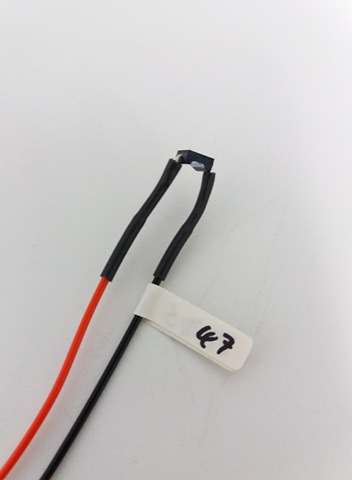
\includegraphics[width = 0.8\linewidth]{Photodiode.jpg}
            \caption{\scriptsize Example of a wired BPW34F photodiode.}
            \end{figure}
        \end{minipage}
    \end{frame}
        
    \begin{frame}{What is a Photodiode?}
        \begin{figure}
            \centering
            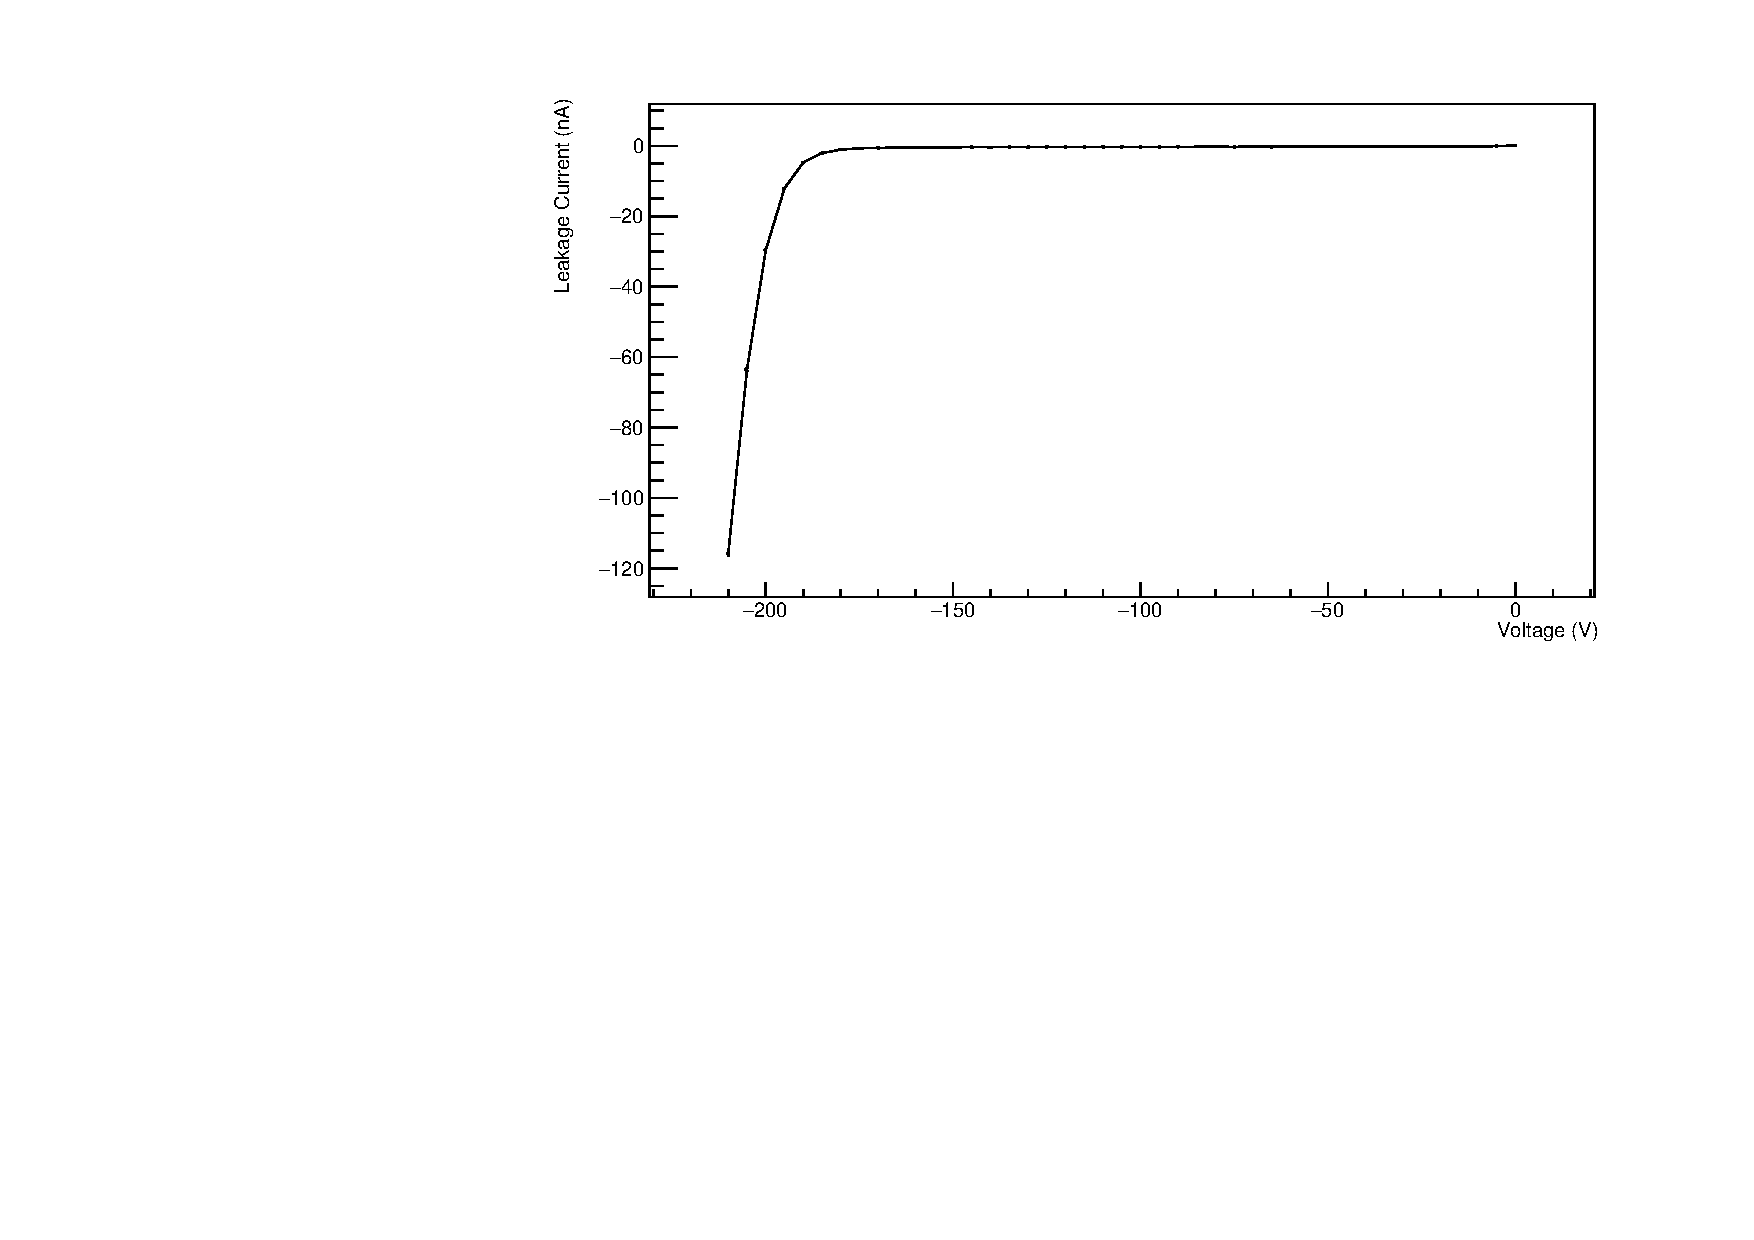
\includegraphics[width=0.9\linewidth]{Diode39_IV_2602.pdf}
            \caption{Reverse bias I--V curve for a non-irradiated diode.}
            \label{fig:Diode39IV}
        \end{figure}  
    \end{frame}
    
    \begin{frame}{What is a Photodiode?}{The Depletion Region}
        \begin{minipage}{0.6\linewidth}
            \begin{figure}
                \centering
                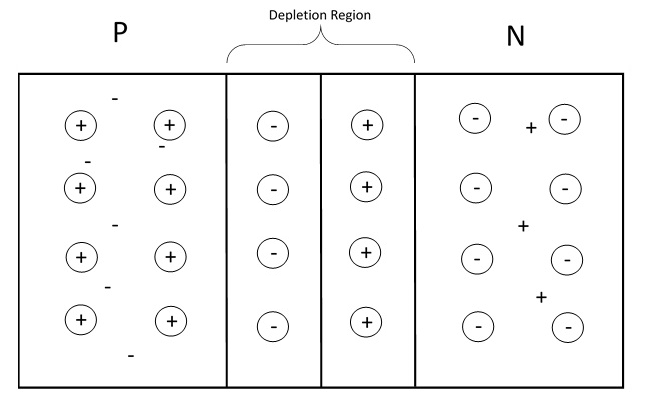
\includegraphics[width = 0.9\linewidth]{PNJunctionDepletion.png}
                \caption{Diagram of a P--I--N junction under reverse bias (positive terminal is on the right).}
                \label{fig:Depletion}
            \end{figure}
        \end{minipage}%
        \begin{minipage}{0.4\linewidth}
            \begin{itemize}
                \item Analogous to a parallel plate \textbf{capacitor}.
                \vspace{0.5cm}
                \item Size of the \textbf{depletion region} grows as higher voltages are applied.
                \vspace{0.5cm}
                \item The depletion region ceases to grow when \textbf{maximum depletion voltage} is reached.
            \end{itemize}
        \end{minipage}
    \end{frame}

\section{Experimental Procedure}
\subsection{I--V Measurements}
    
    \begin{frame}{I--V Measurements}{Setup}
        \begin{figure}
            \centering
            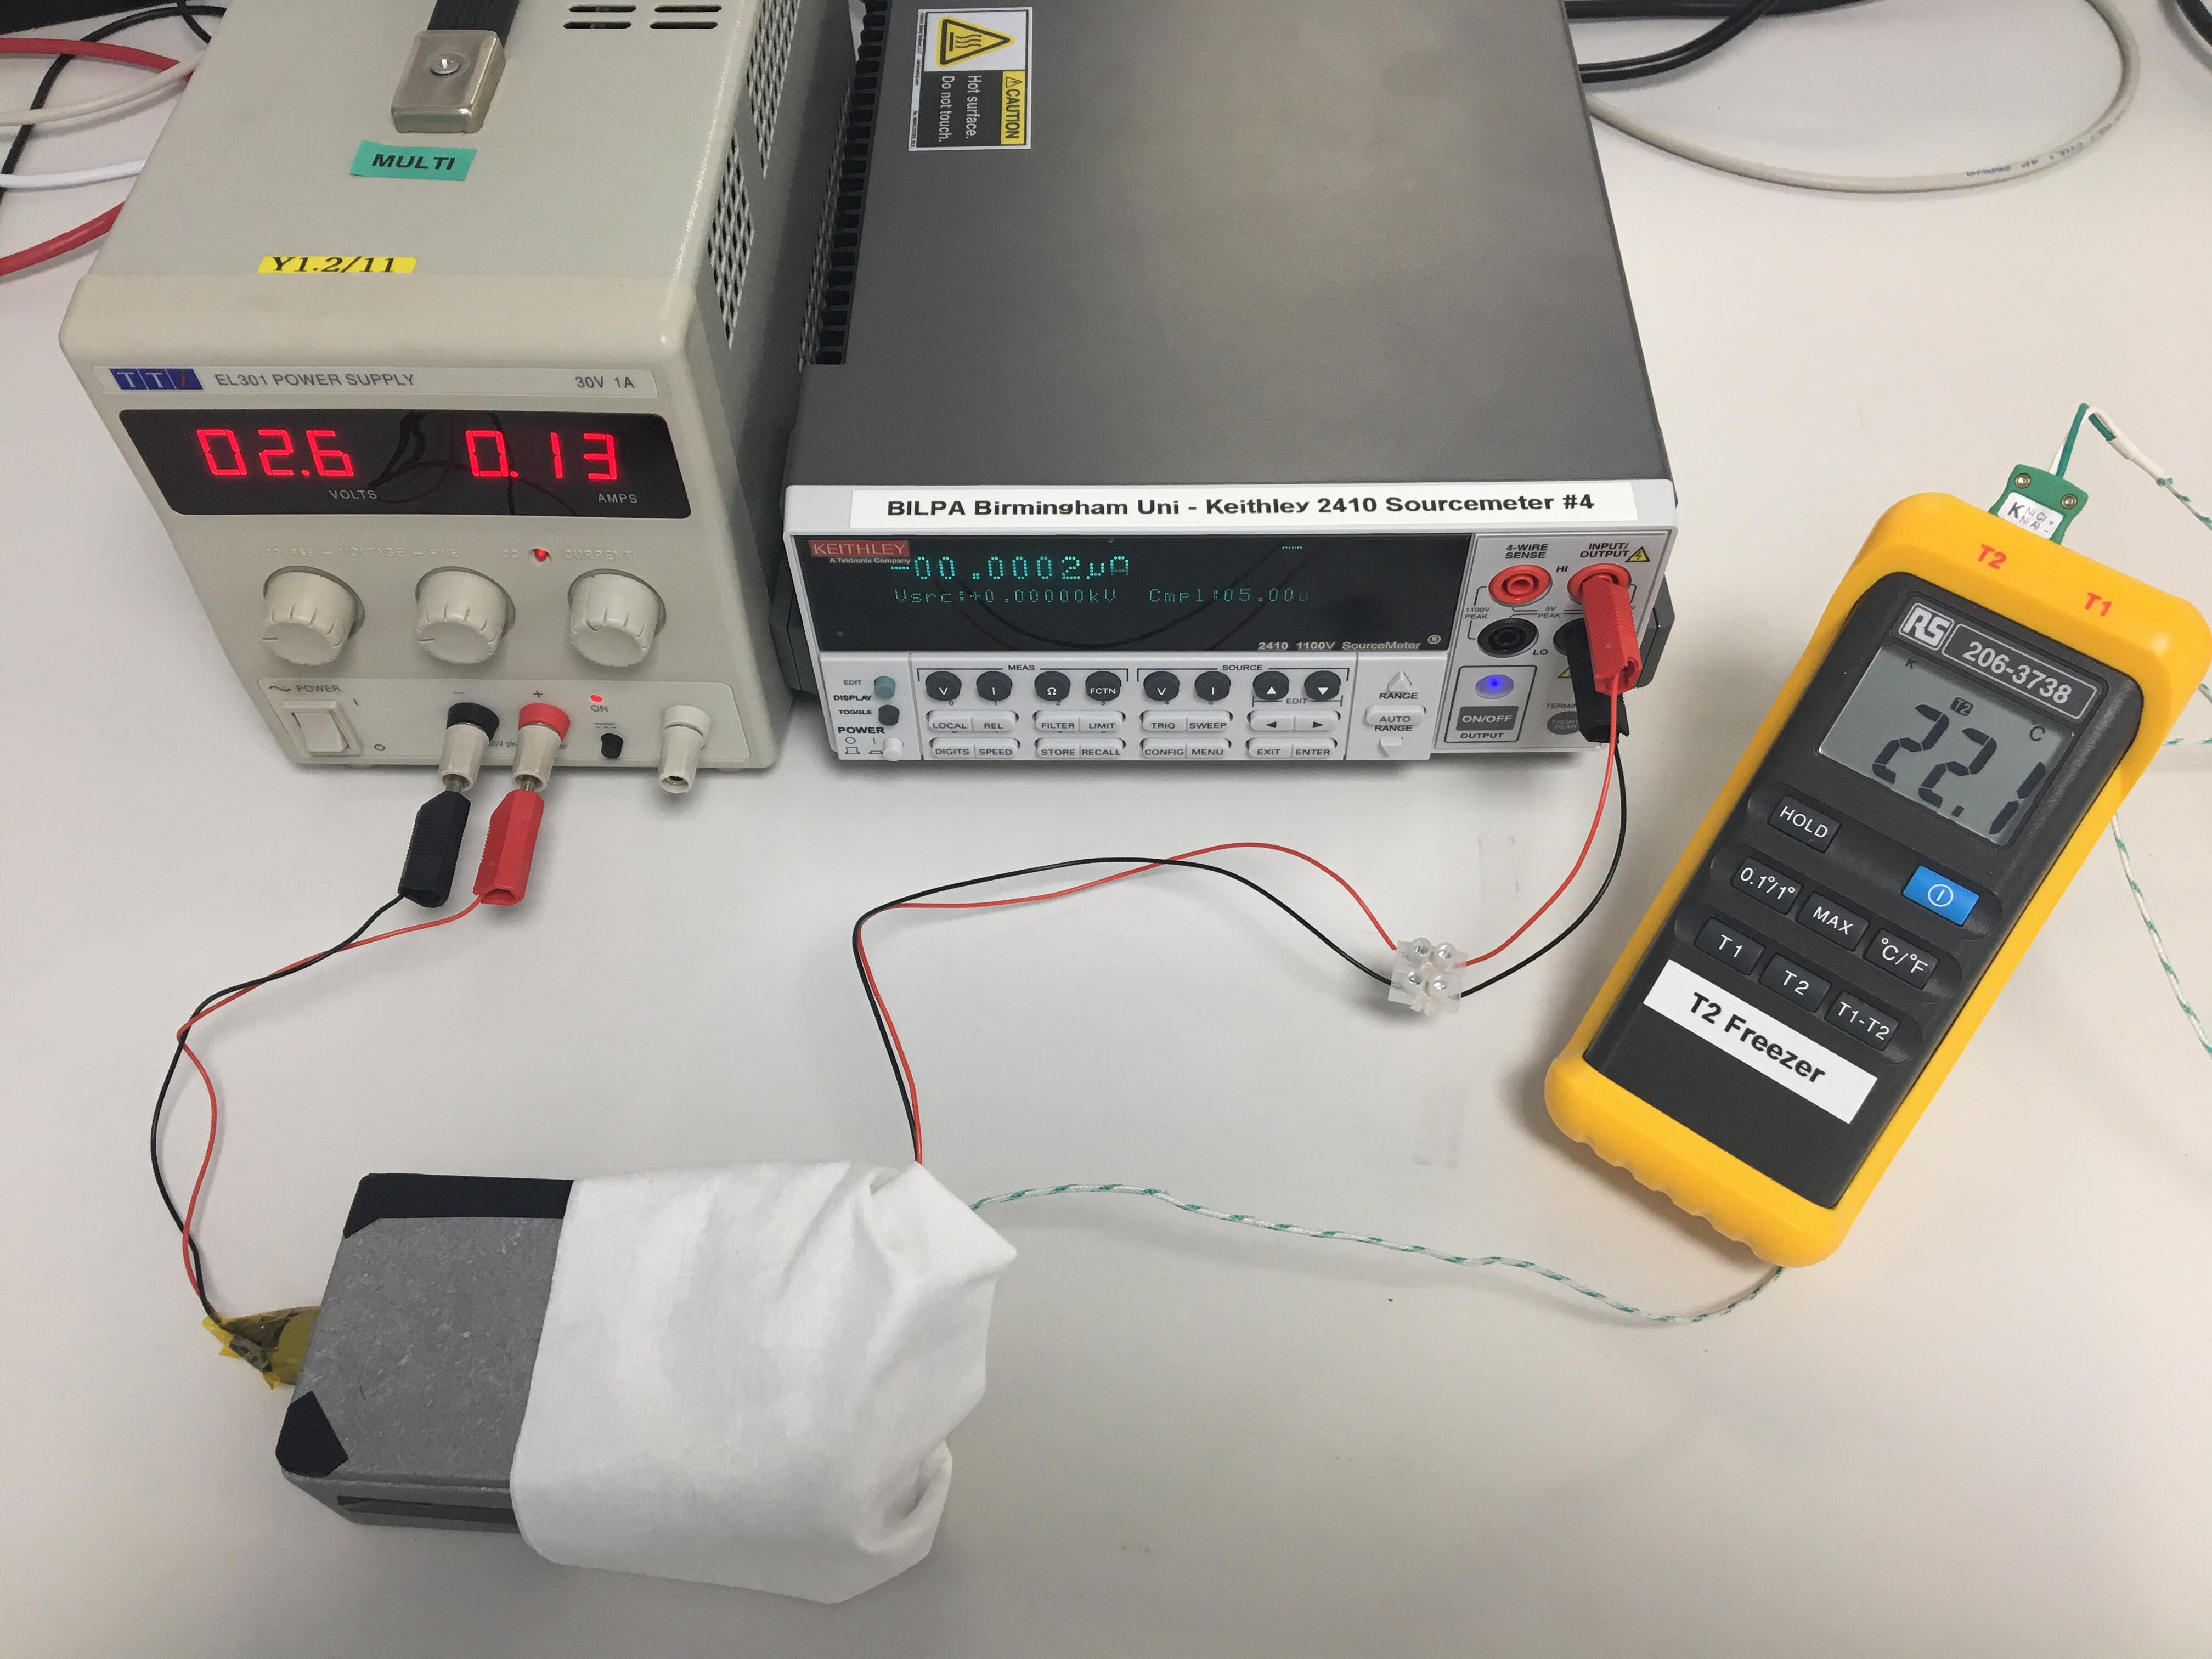
\includegraphics[width = 0.7\linewidth]{IV_Setup.jpg}
            \caption{Experimental setup for I--V measurements.}
            \label{fig:IVSetup}
        \end{figure}
    \end{frame}
    
    \begin{frame}{I--V Measurements}{Setup}
        \begin{figure}
            \centering
            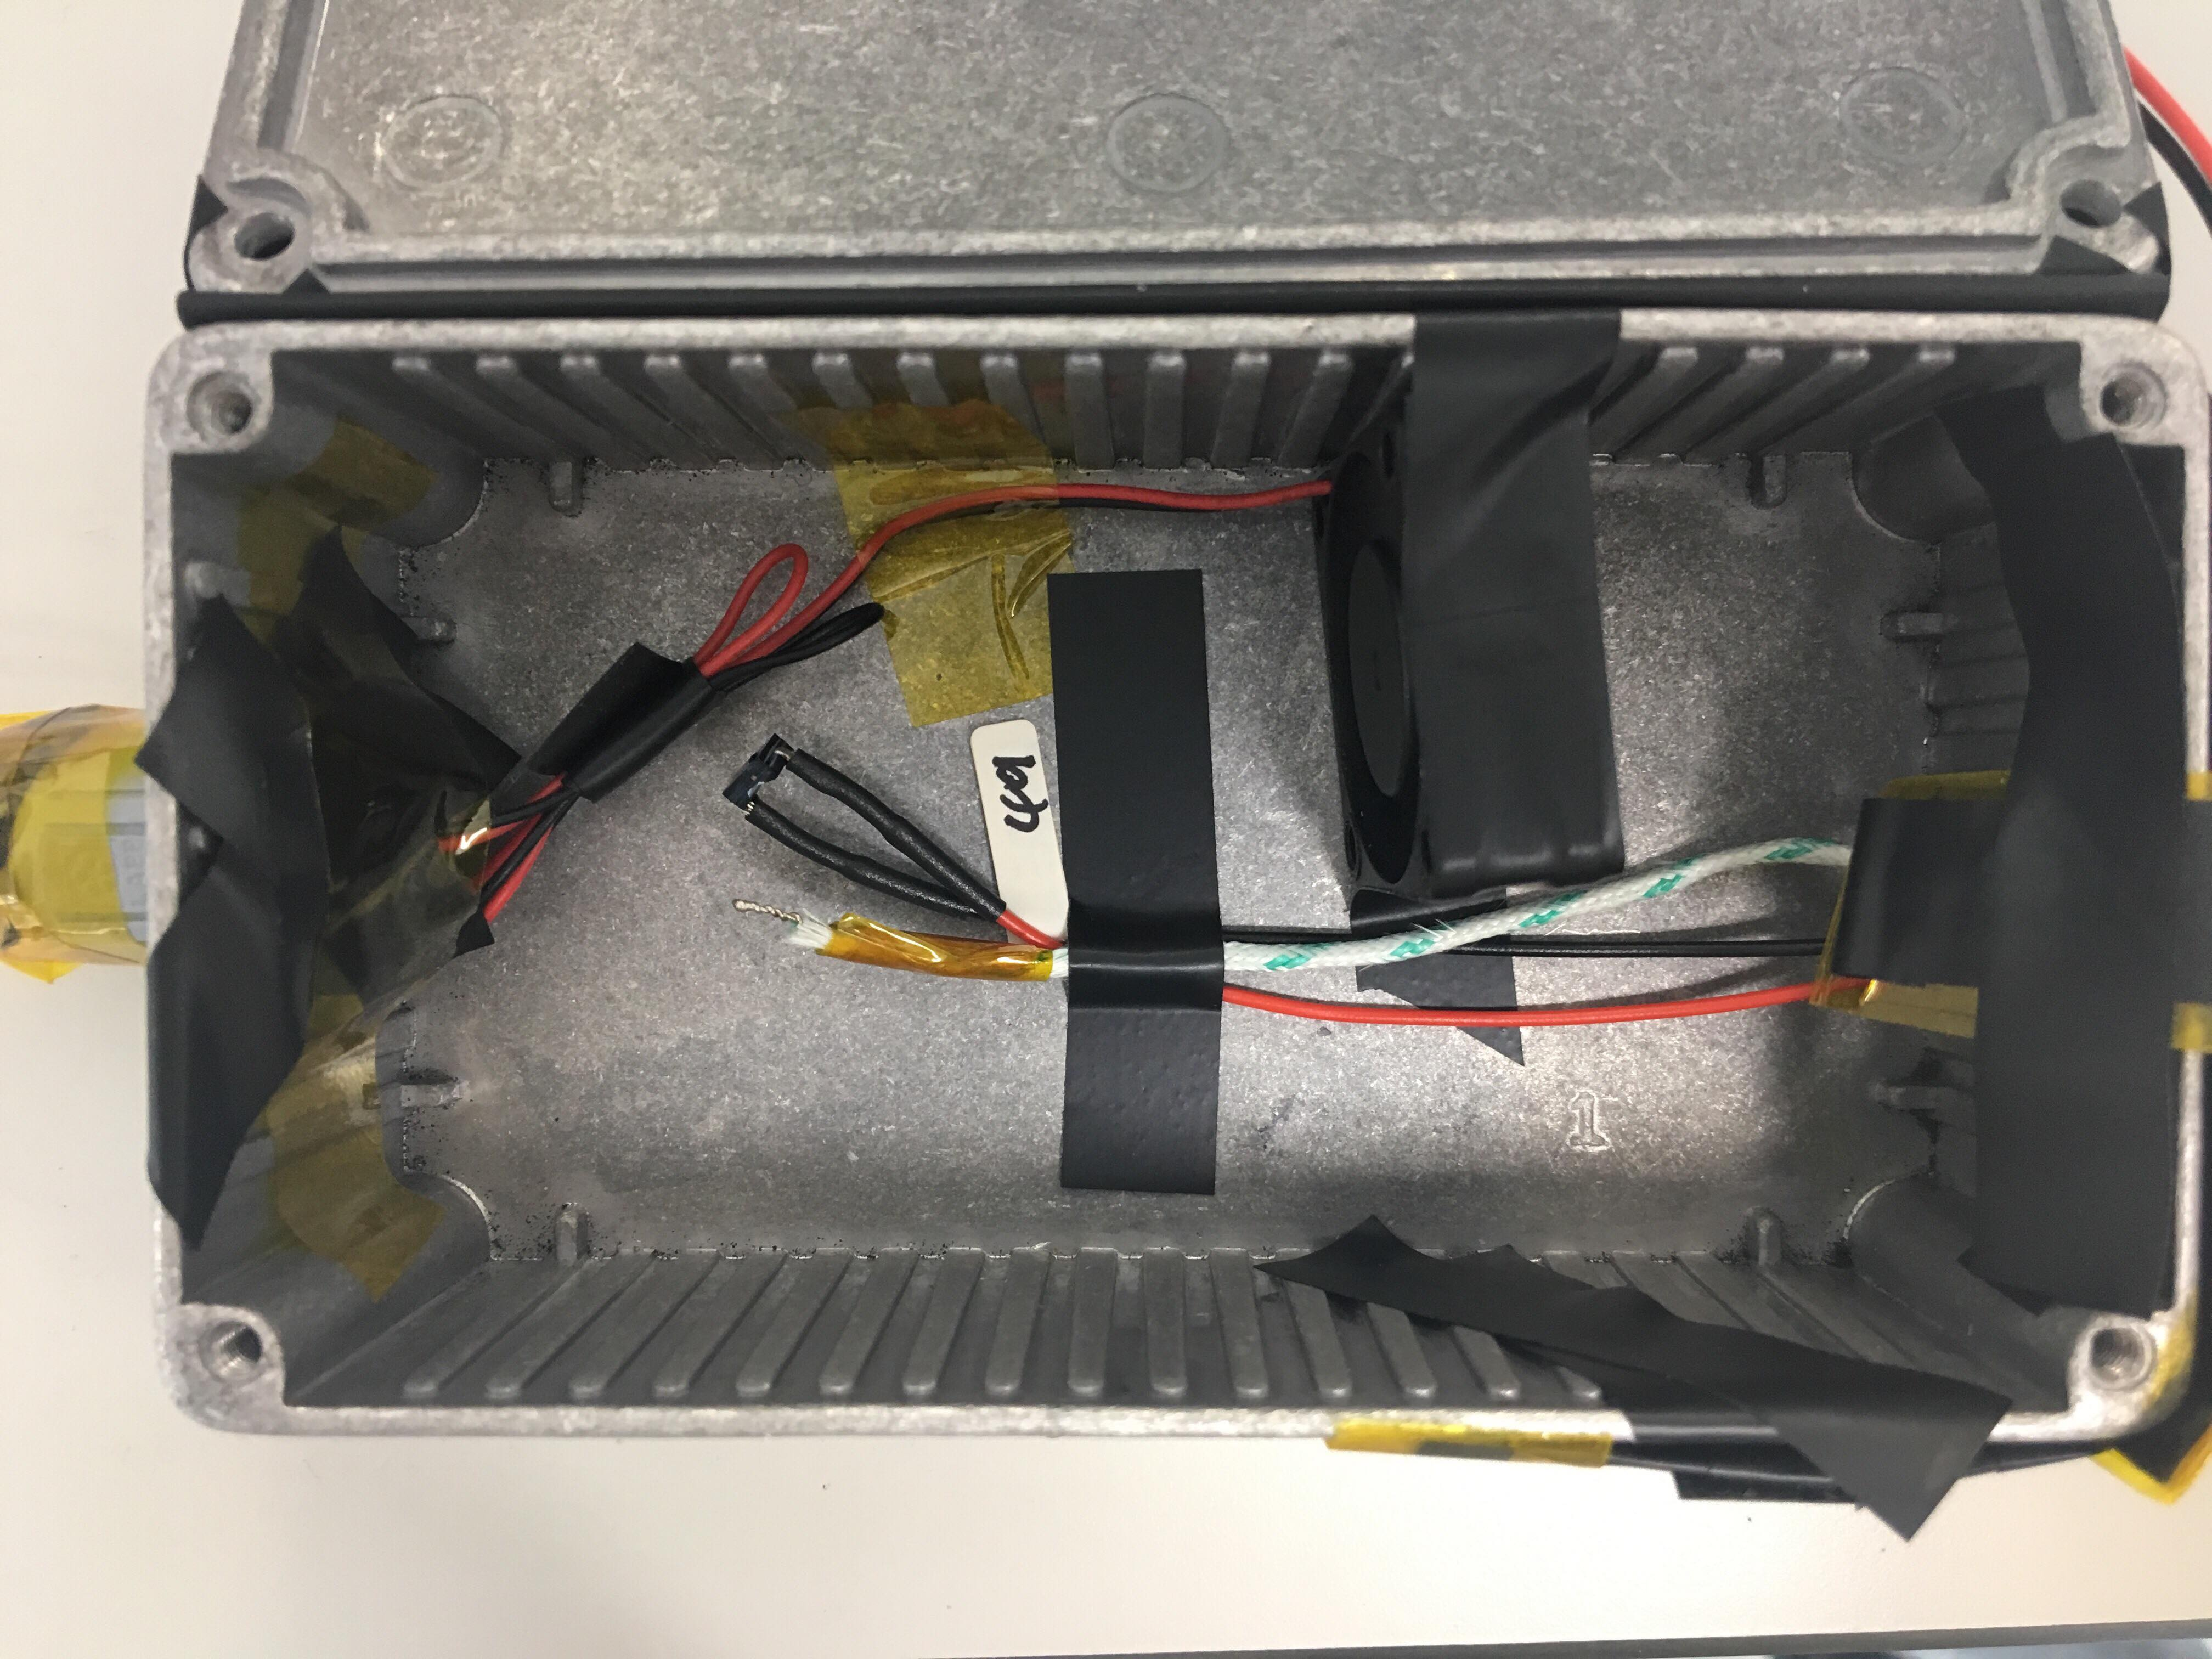
\includegraphics[width = 0.7\linewidth]{Photodiode_Box.jpg}
            \caption{Aluminium shielding box.}
            \label{fig:IVbox}
        \end{figure}
    \end{frame}
    
    \begin{frame}{I--V Measurements}{Temperature Dependence of Leakage Current}
        \begin{itemize}
            \item The \textbf{leakage current} of a photodiode is dependent on \textbf{temperature} by \textsuperscript{\cite{Moll}}:
                \begin{equation*}
                    I(T_R) = I(T) \left(\frac{T_R}{T}\right)^2e^{-\frac{E_a}{2k_B}\left[\frac{1}{T_R}-\frac{1}{T}\right]}
                \end{equation*}
            \item Therefore, all I--V measurements were scaled to a \textbf{reference temperature} of 21${}^\circ$C.
        \end{itemize}
    \end{frame}
    
    \begin{frame}{I--V Measurements}{Effect of Temperature Scaling}
        \begin{figure}
            \centering
            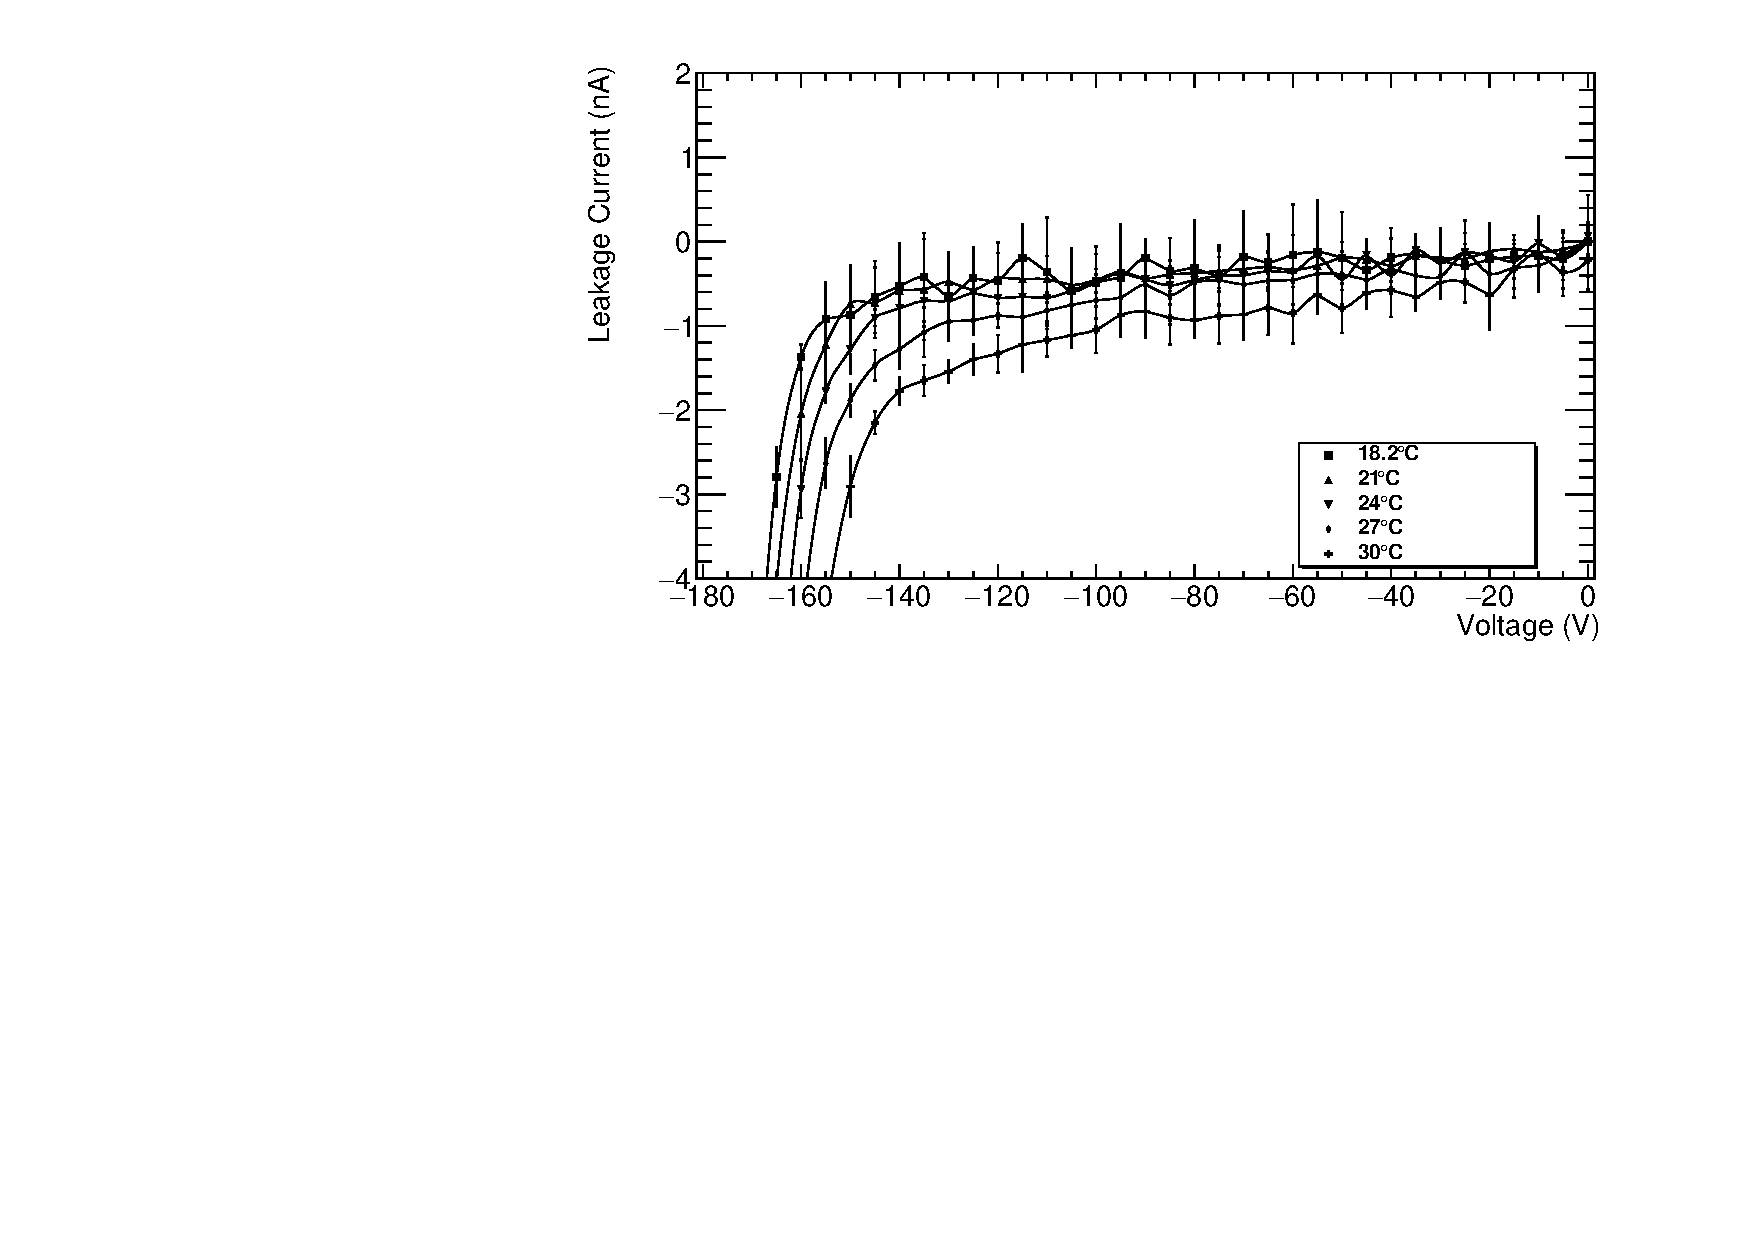
\includegraphics[width=0.9\textwidth]{Unscaled_IV_0503_bigpoints.pdf}
            \caption{\footnotesize I--V curves before temperature scaling.}
            \label{fig:NonScaledIVCurves}
        \end{figure}
    \end{frame}
    
    \begin{frame}{I--V Measurements}{Effect of Temperature Scaling}
        \begin{figure}
            \centering
            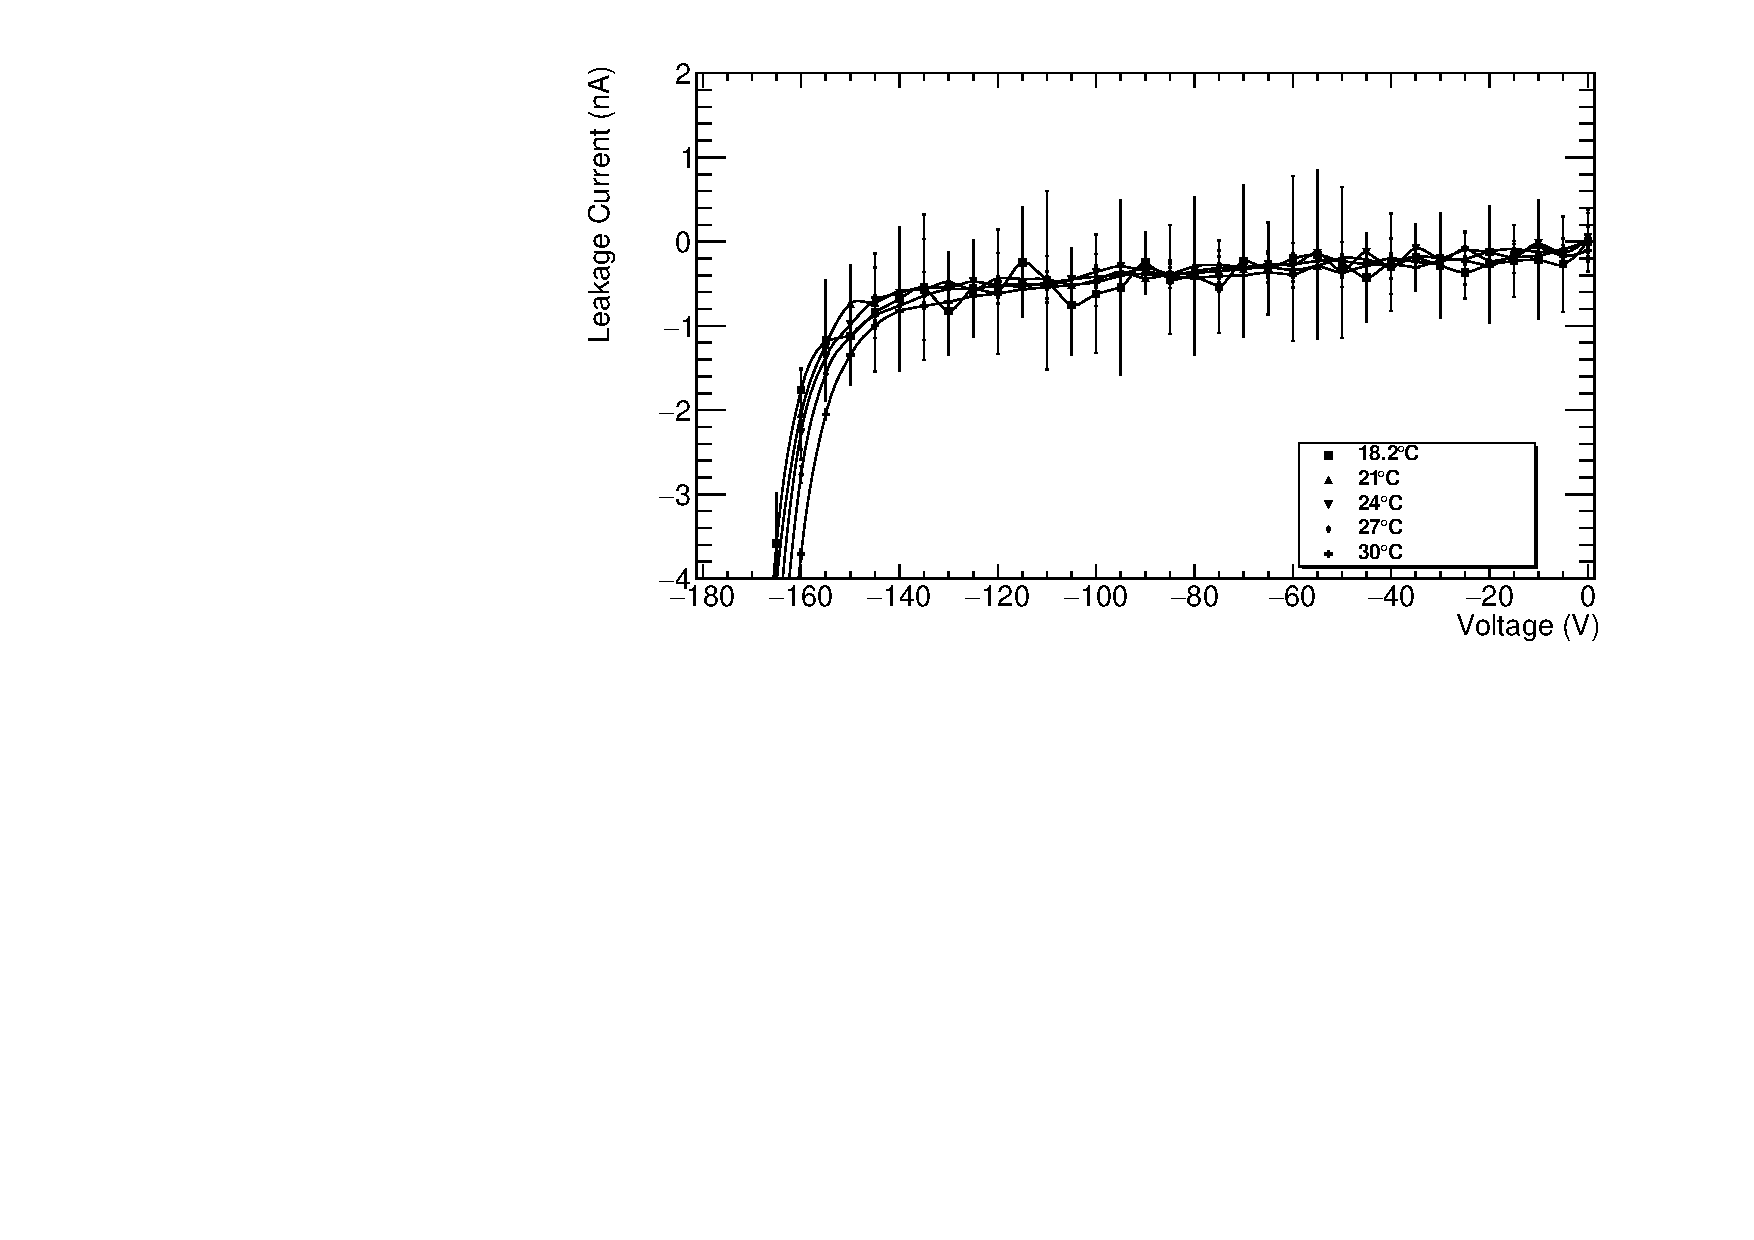
\includegraphics[width=0.9\textwidth]{Scaled_IV_0503_bigpoints.pdf}
            \caption{\footnotesize I--V curves after temperature scaling.}
            \label{fig:ScaledIVCurves}
        \end{figure}
    \end{frame}
    
    \begin{frame}{I--V Measurements}{Calculating the Activation Energy}
        \begin{itemize}
            \item The range of $15^{\circ}$C $<T<30^{\circ}$C was investigated.% further, and the errors were minimized.
        \end{itemize}
        \vspace{-0.5cm}
        \begin{figure}
            \centering
            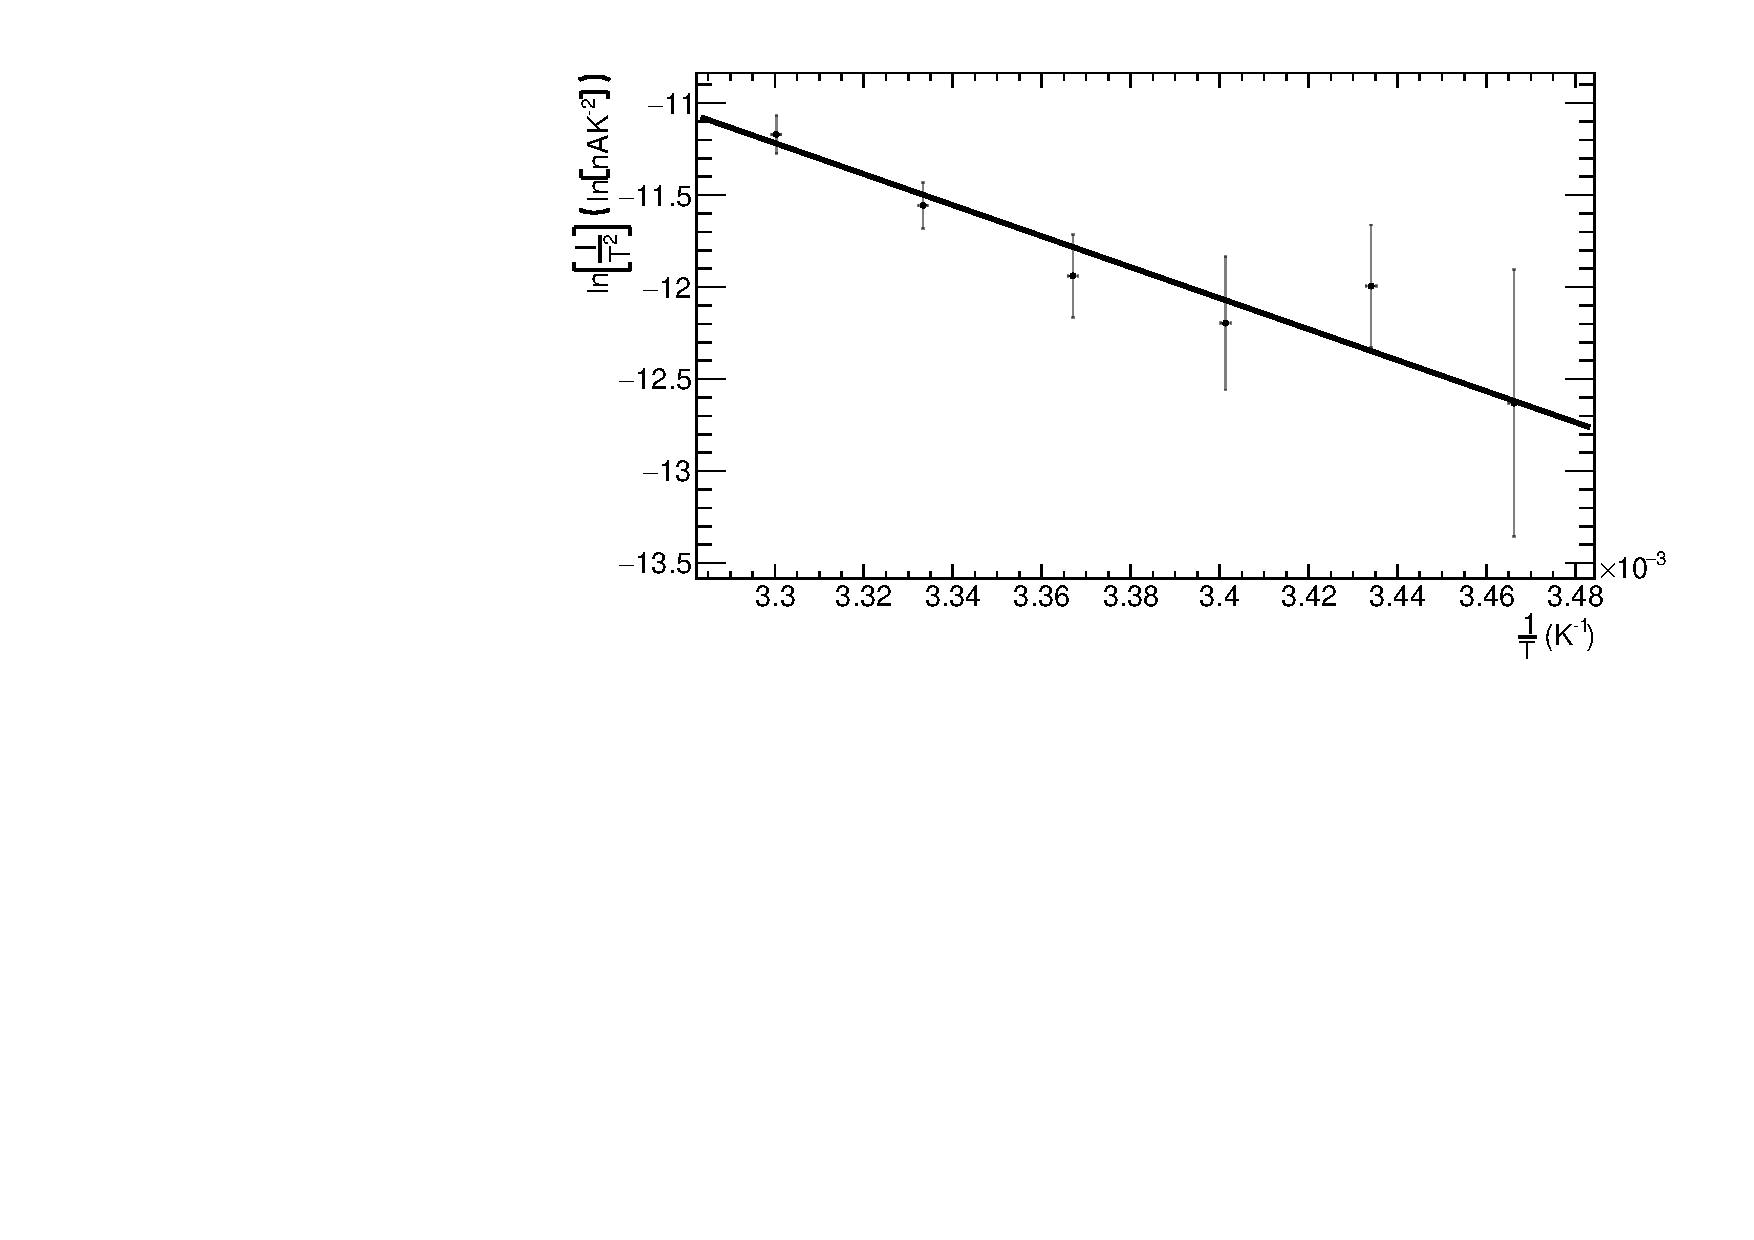
\includegraphics[width = 0.75\linewidth]{BandGap_0503.pdf}
            \caption{$\ln \left[{\frac{I}{T^2}}\right]$ vs $\frac{1}{T}$ in the range $10^{\circ}$C $<T<35^{\circ}$C.}
            \label{fig:my_label}
        \end{figure}
        \vspace{-0.5cm}
        \begin{itemize}
        \item This yields a value of $\bm{E_a = 1.45 \pm 0.33}$ \textbf{eV}.
        \end{itemize}
    \end{frame}
    
\subsection{C--V Measurements}
    
    \begin{frame}{C--V Measurements}{Current -- Voltage Relation and Maximum Depletion Voltage.}
        \begin{itemize}
            \item The \textbf{capacitance} of a photodiode is related to the \textbf{reverse bias} by \textsuperscript{\cite{Casse}}:
                \begin{equation*}
                    C = \frac{f\sqrt{\epsilon_{Si}\epsilon_0}}{\sqrt{V}}
                \end{equation*}
            \item At \textbf{maximum depletion voltage}, capacitance becomes independent of voltage.
            \vspace{0.5cm}
            \item Plotting \textbf{capacitance vs voltage} on a log plot should therefore show a straight line, with a \textbf{deviation} at maximum depletion.
        \end{itemize}
    \end{frame}
    
    \begin{frame}{C--V Measurements}{Setup}
        \begin{figure}
            \centering
            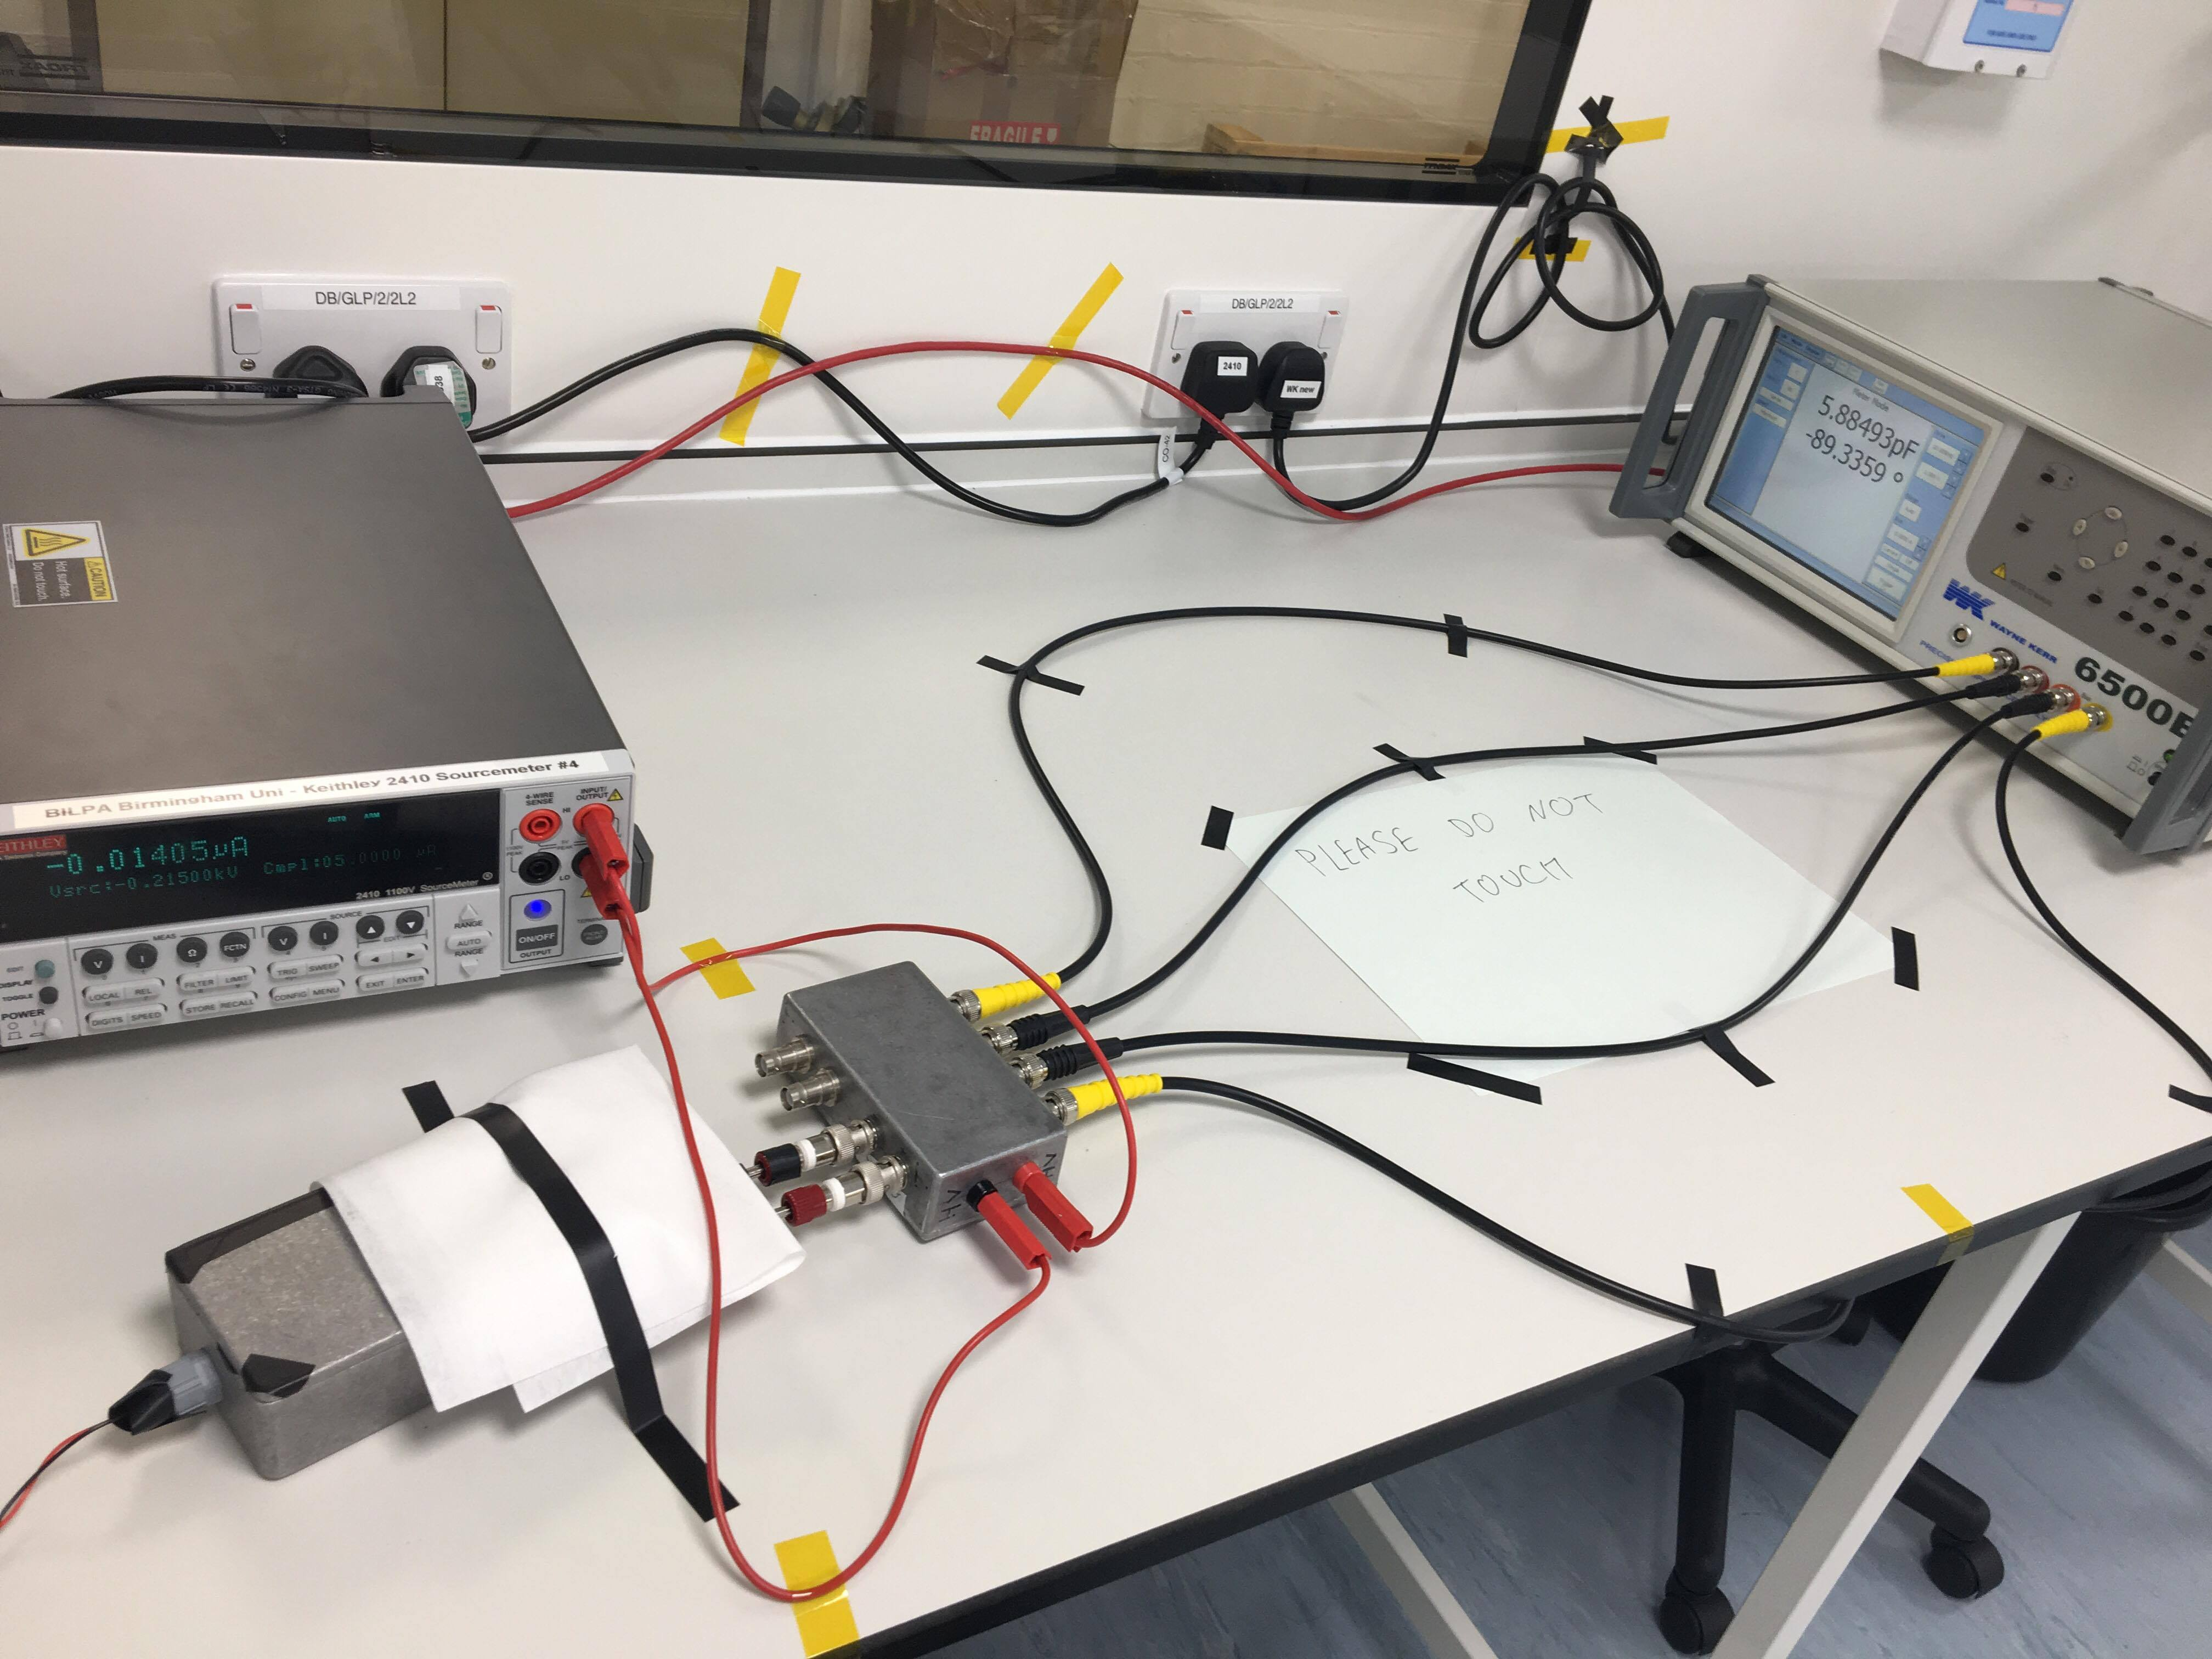
\includegraphics[width = 0.8\linewidth]{CVSetup.jpg}
            \caption{Experimental setup for C--V measurements.}
            \label{fig:CVSetup}
        \end{figure}
    \end{frame}
    
    \begin{frame}{C--V Measurements}{Calculating Maximum Depletion Voltage}
        \begin{itemize}
            \item By calculating the \textbf{intersect} of the two fits, the point at which the trend deviates from a straight line can be calculated.
            \vspace{0.3cm}
            \item Applying this method, a maximum depletion voltage value of $\bm{V_{dep} = -90.8 \pm 5.1}$ \textbf{V} was inferred. 
        \end{itemize}
        \begin{figure}
            \centering
            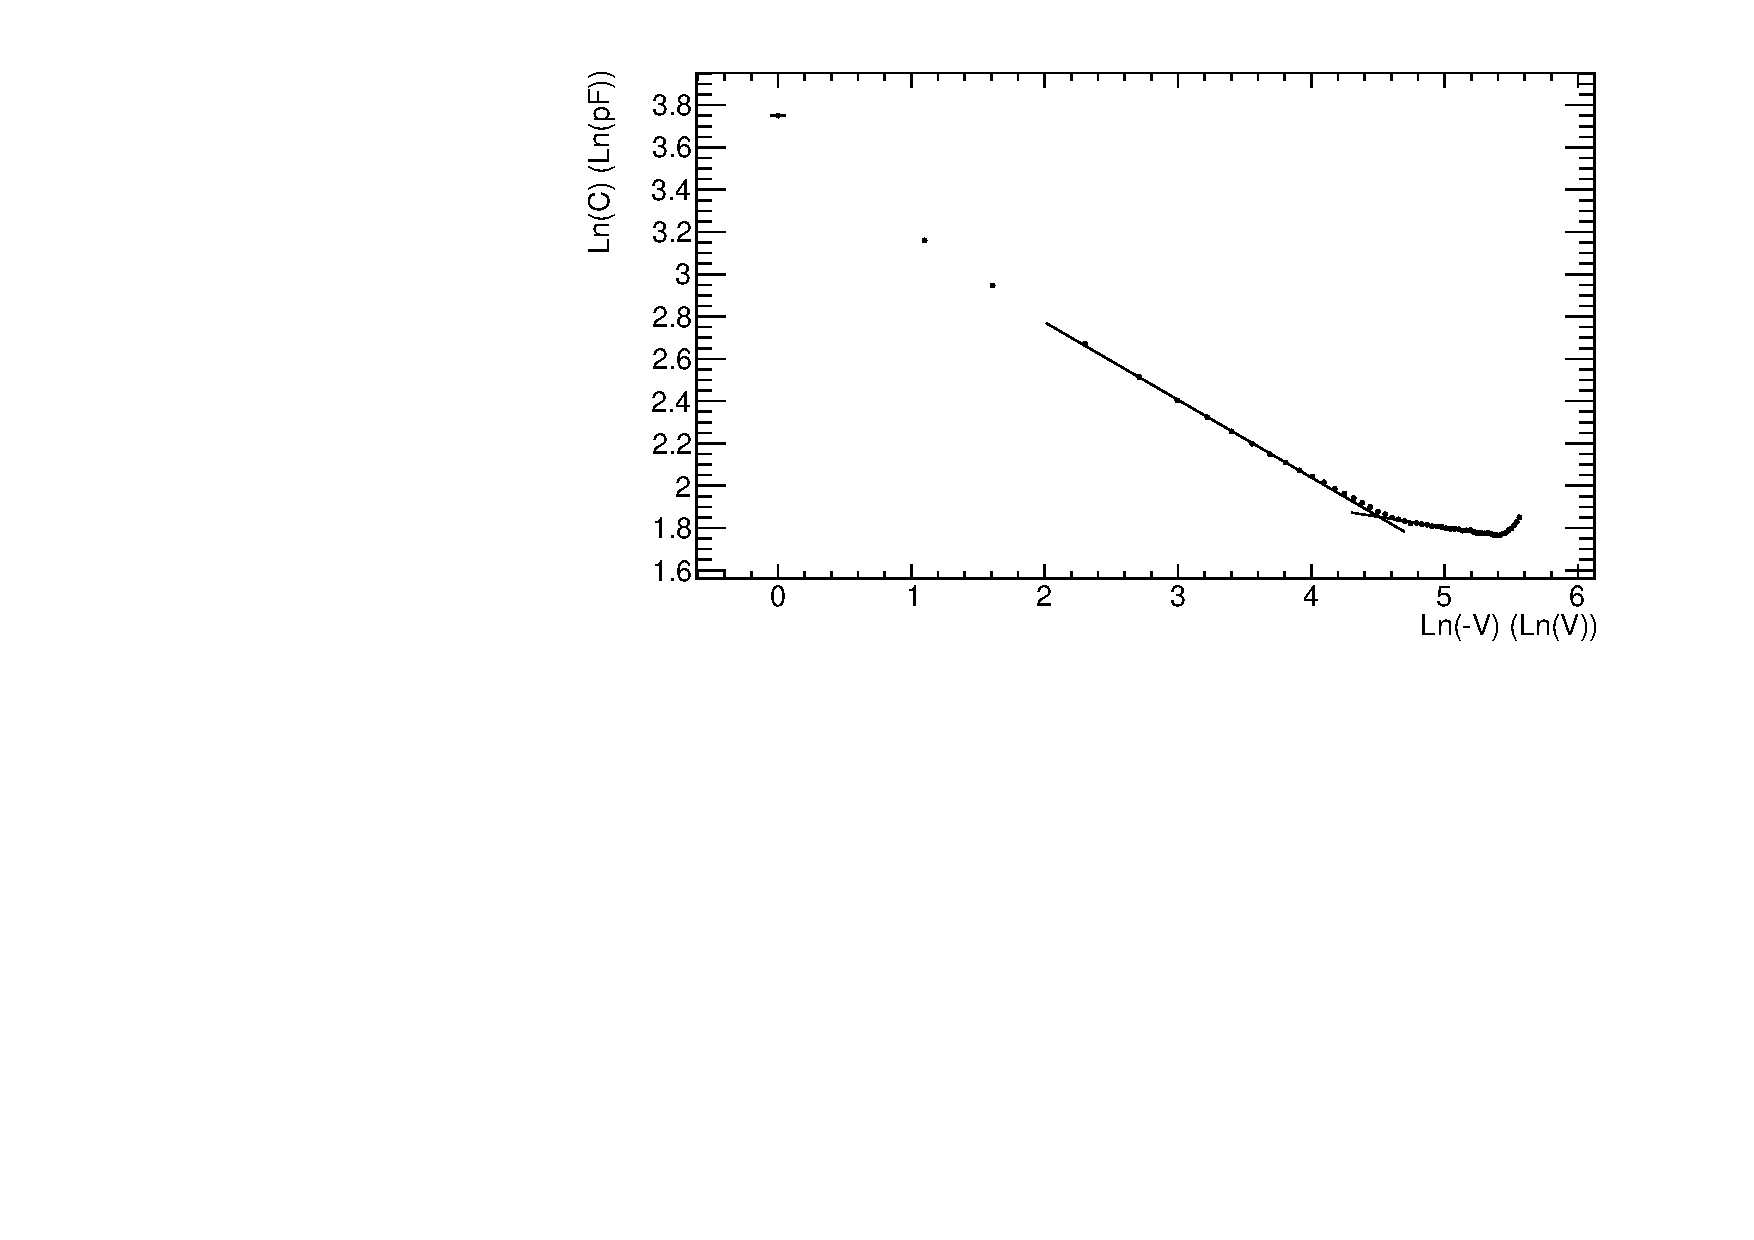
\includegraphics[width = 0.8\linewidth]{Diode2_nonirradiated_CV_noextrapolation_1711.pdf}
            \vspace{-0.4cm}
            \caption{log capacitance vs log voltage.}
            \label{fig:CVNonIrradiated}
        \end{figure}
    \end{frame}
    
\subsection{Proton Irradiations}

    \begin{frame}{Proton Irradiations}{Mounting the Photodiodes}
        \centering
        $\otimes$ Beam direction.
        \begin{figure}
            \begin{minipage}[b]{0.5\linewidth}
            \centering
            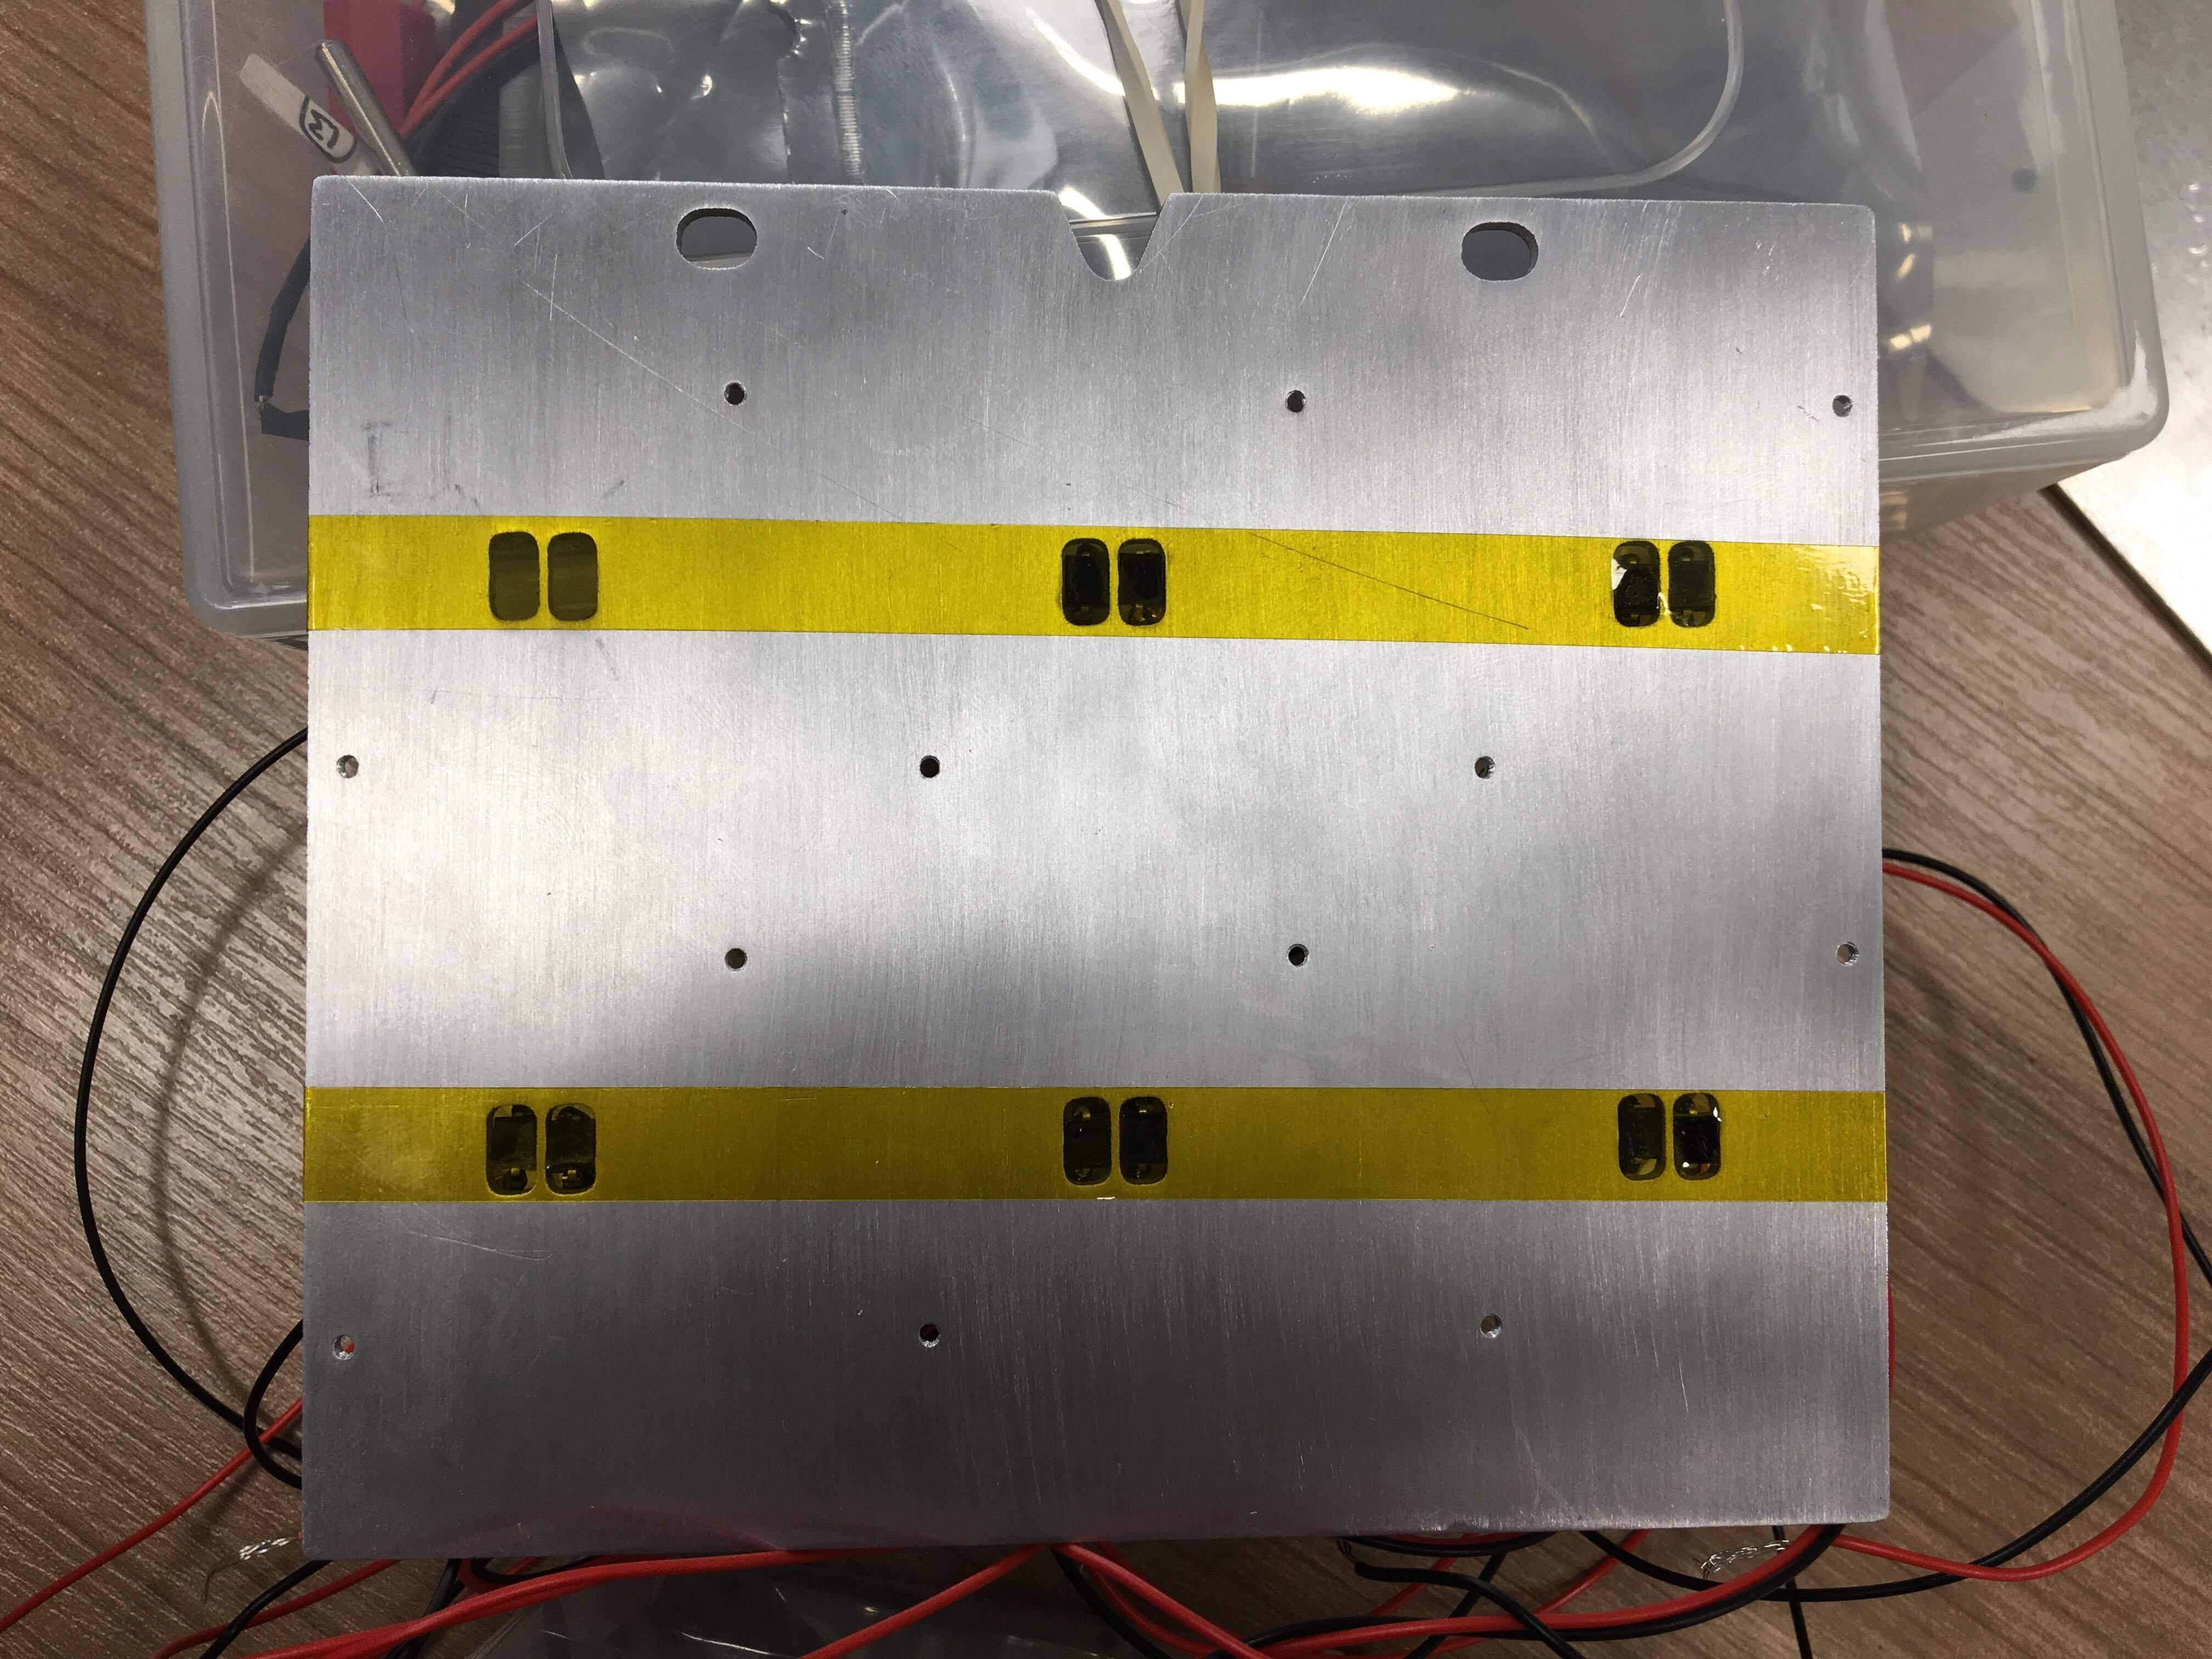
\includegraphics[width = 0.98\textwidth]{Mount_no_Foils.jpg}
        \end{minipage}%
        \begin{minipage}[b]{0.5\linewidth}
            \centering
            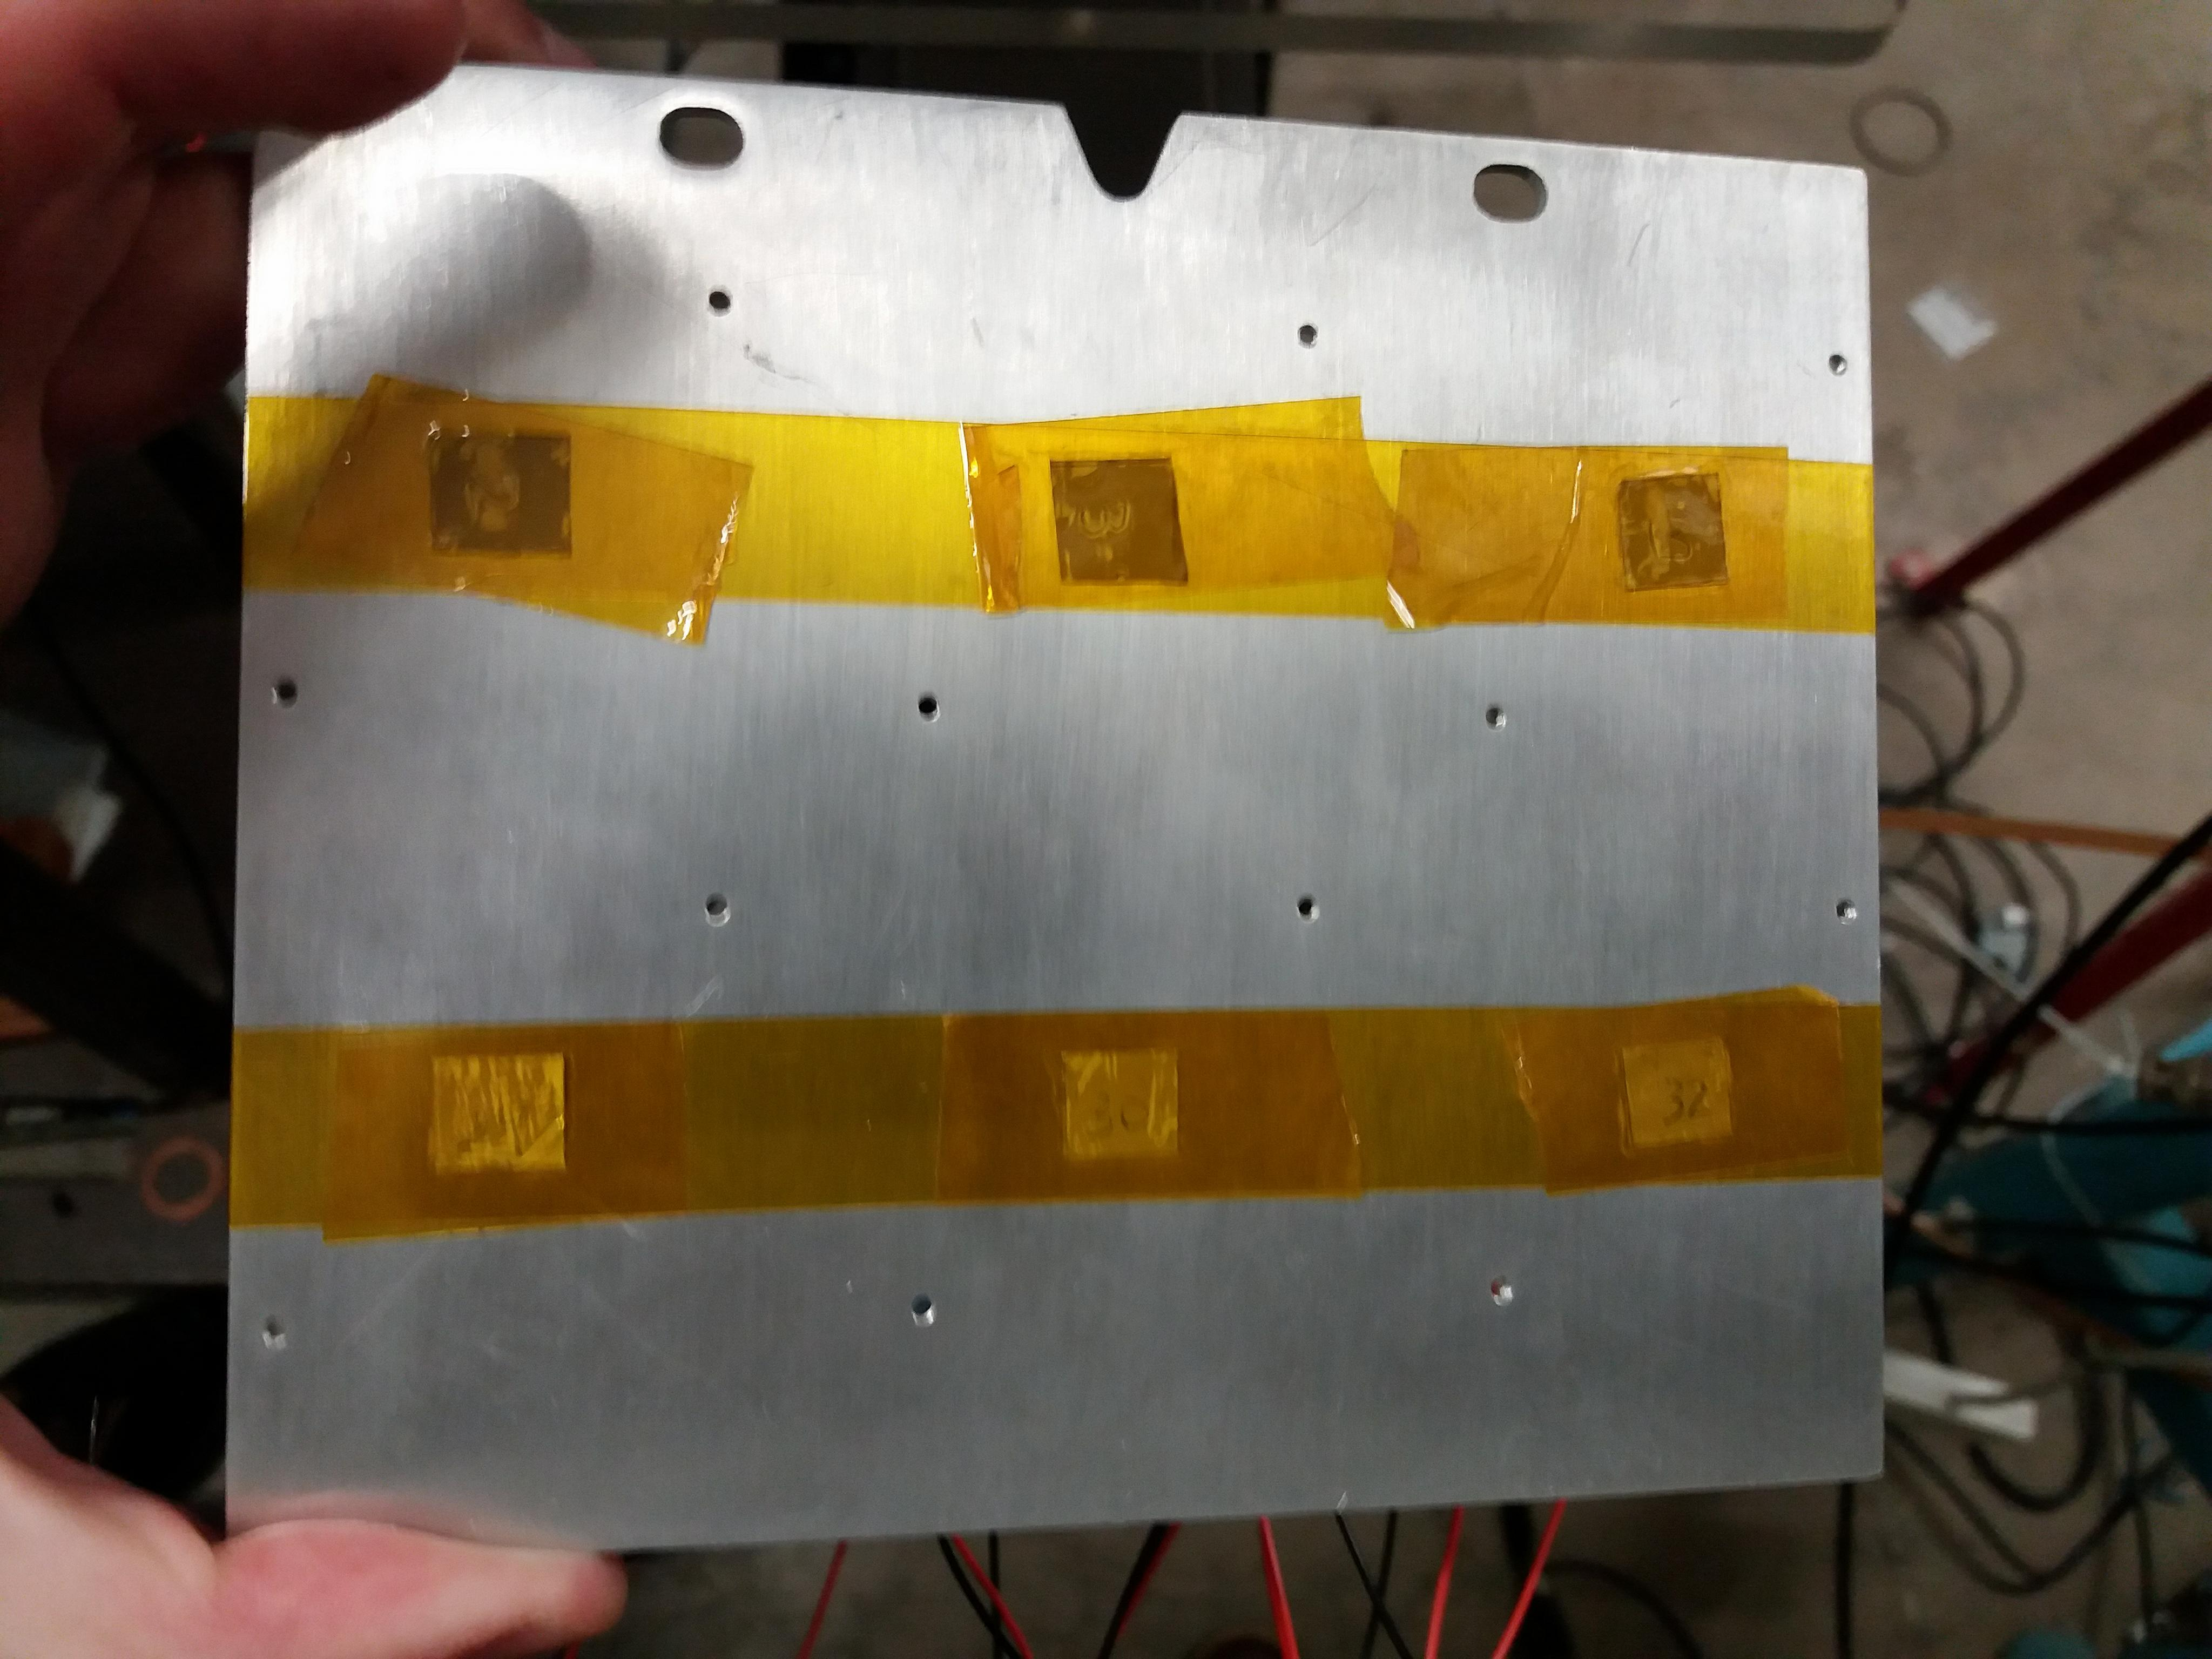
\includegraphics[width = 0.98\textwidth]{Mount_with_Foils.jpg}
        \end{minipage}
        \end{figure}
        \centering
        Aluminium mount. The nickel foils were used to measure the incident fluence.
    \end{frame}
        
    \begin{frame}{Proton Irradiations}{The Isolation Box}
        \begin{figure}
            \begin{minipage}[b]{0.5\linewidth}
            \centering
            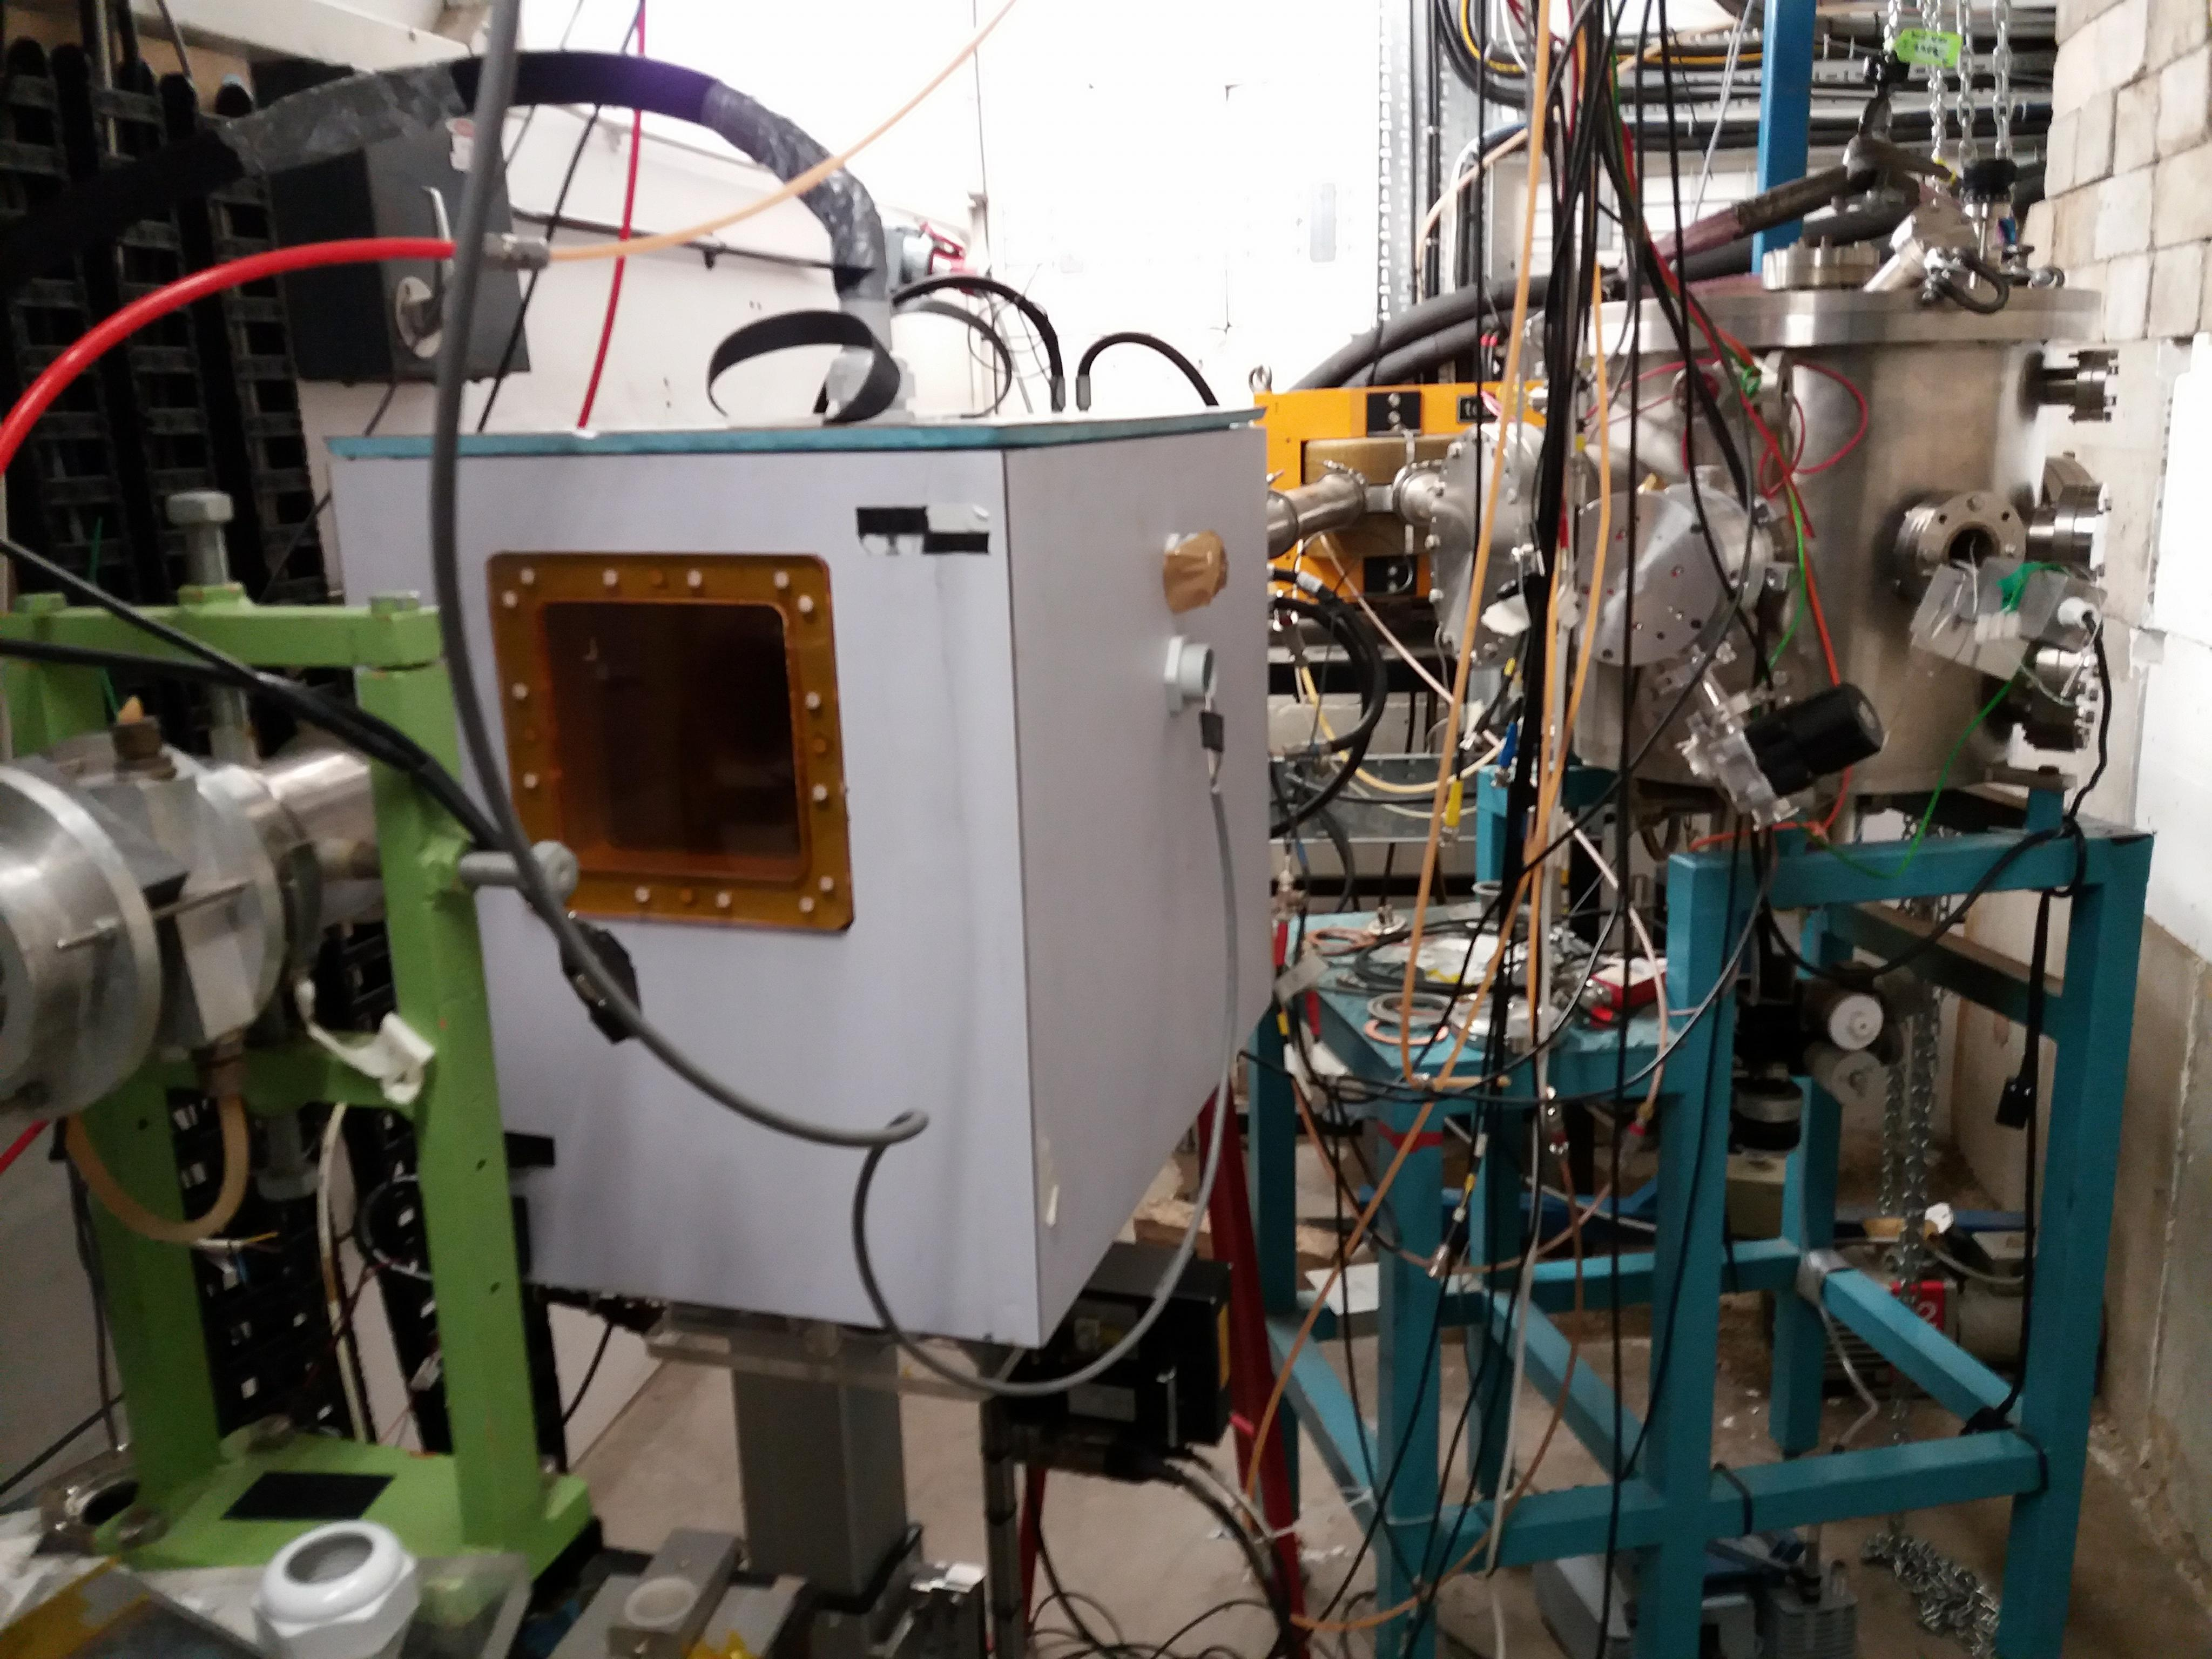
\includegraphics[width = 0.98\textwidth]{ATLAS_chamber.jpg}
        \end{minipage}%
        \begin{minipage}[b]{0.5\linewidth}
            \centering
            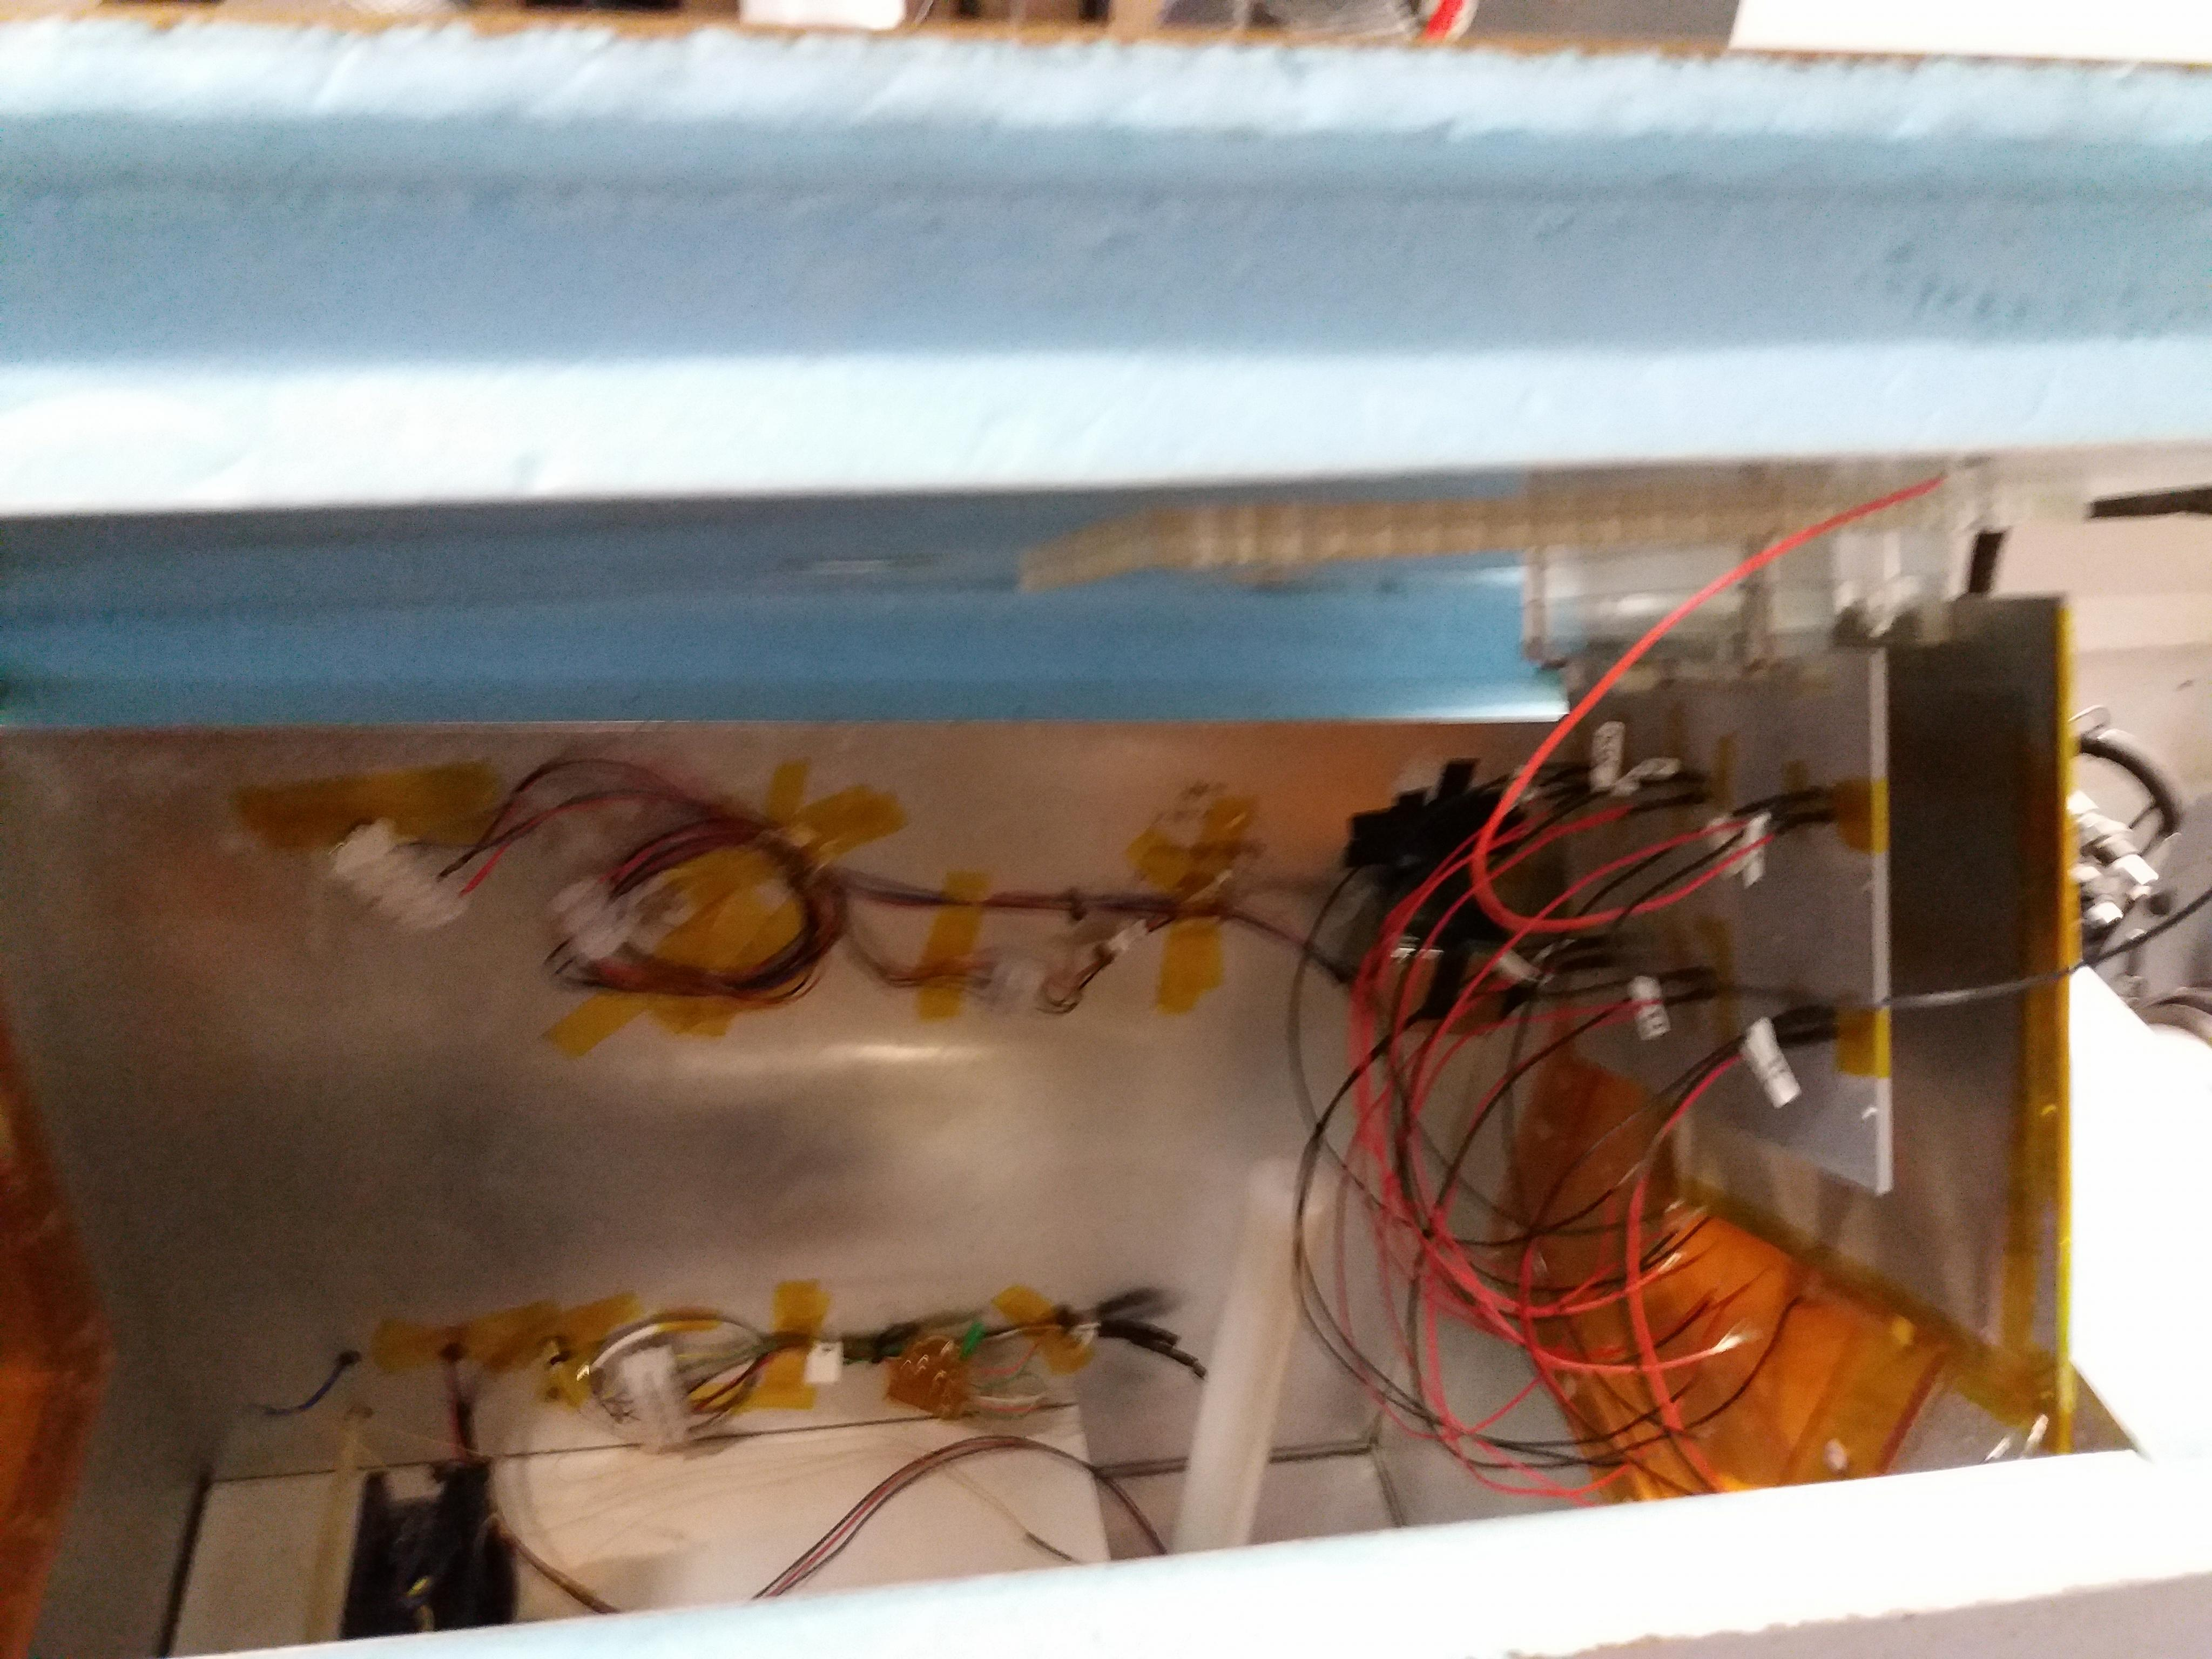
\includegraphics[width = 0.98\textwidth]{Isolation_box.jpg}
        \end{minipage}
        \end{figure}
        The isolation box within the ATLAS chamber, the box was used to cool the photodiodes to $-27^{\circ}$C.
    \end{frame}
    
    \begin{frame}{Proton Irradiations}{Ni Foil Analysis}
        \begin{minipage}{0.45\linewidth}
            \begin{figure}
                \centering
                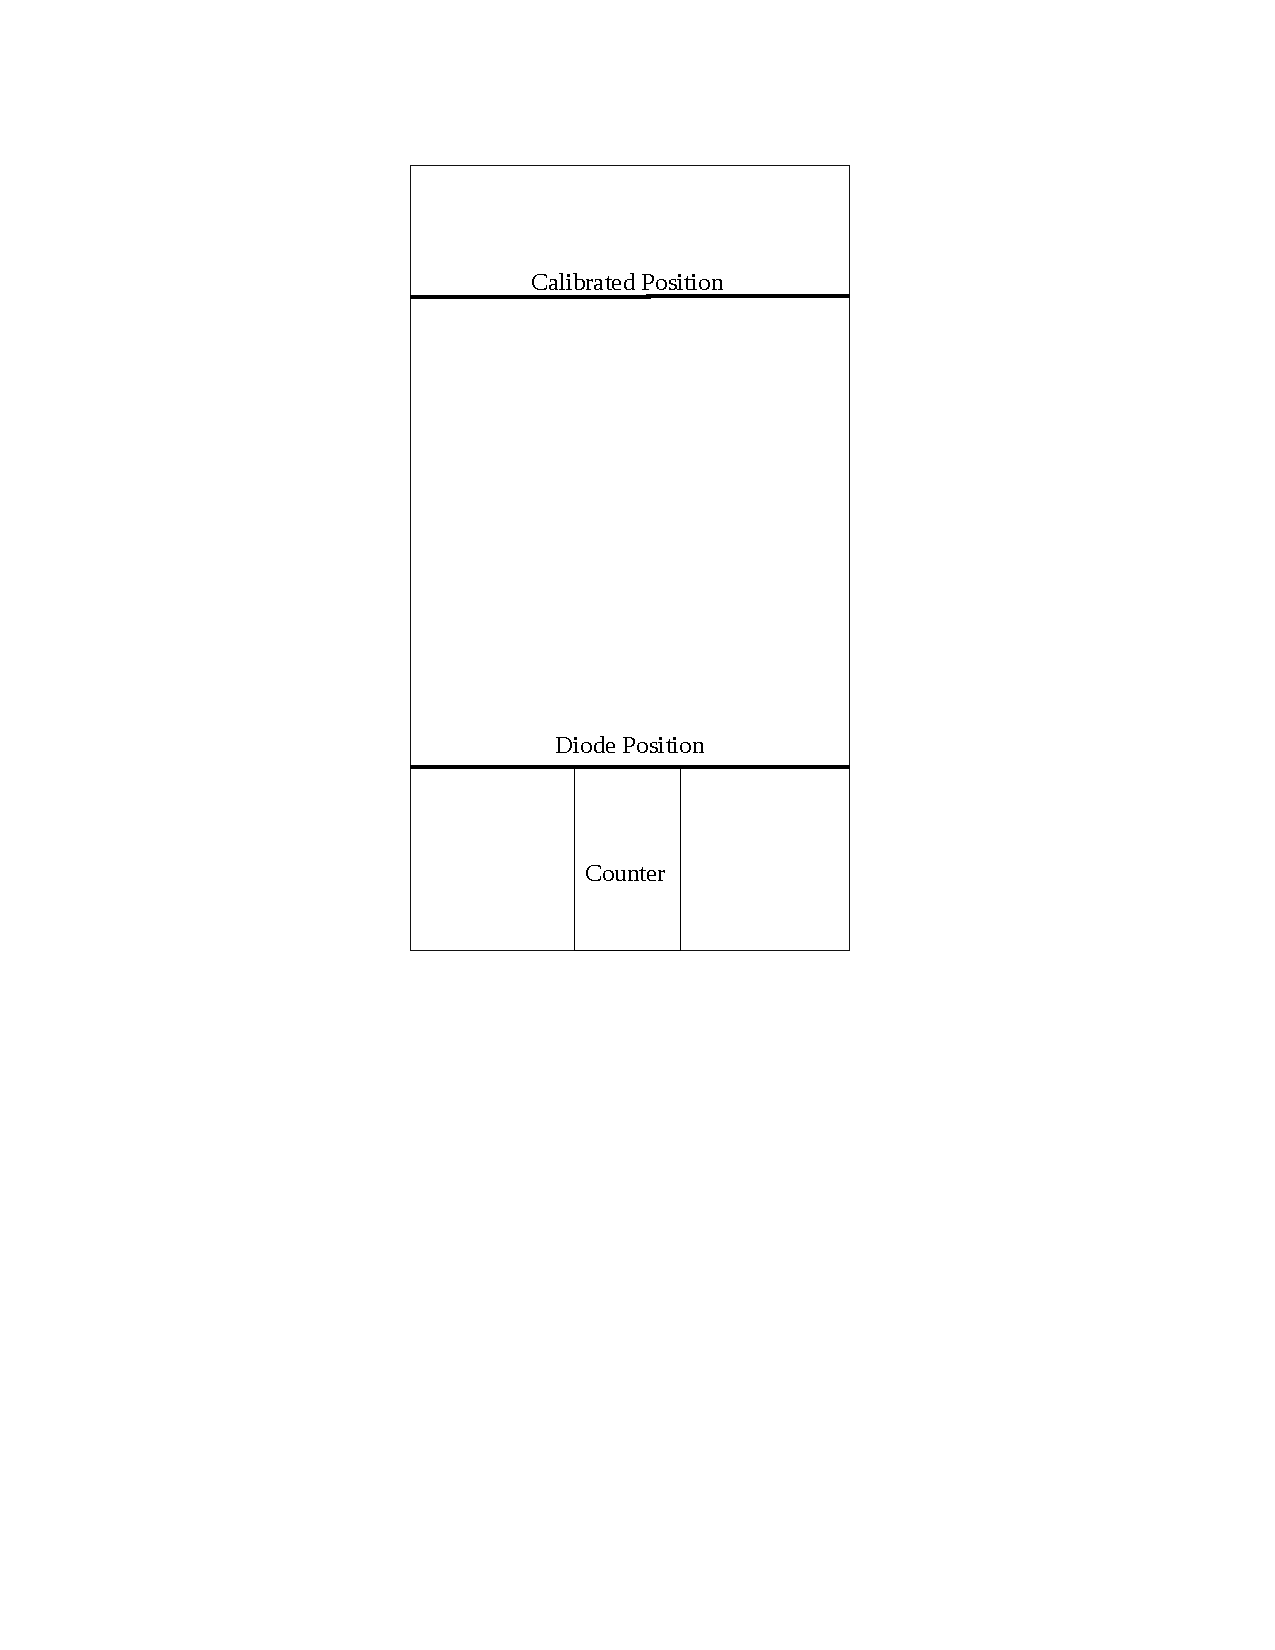
\includegraphics[width = 0.9\linewidth, trim = {6.5cm 11.5cm 5.5cm 2cm}, clip = true]{Counter.pdf}
                \caption{\footnotesize Schematic diagram of germanium counter.}
            \end{figure}
        \end{minipage}%
        \begin{minipage}{0.55\linewidth}
            \begin{itemize}
                \item The \textbf{irradiated nickel foils} were analyzed using a \textbf{germanium counter}.
                \item Due to the weak activity of the foils, they had to be placed directly on top of the counter.
                \item A \textbf{ratio of counts} was taken between this position and the calibrated position.
                \item The measured counts from the foils were then converted into \textbf{proton fluences}.
            \end{itemize}
        \end{minipage}%
    \end{frame}

\subsection{Annealing}    

    \begin{frame}{Annealing}{The Arrhenius Relation}
        \begin{itemize}
            \item A radiation damaged photodiode will \textbf{repair} itself over time.
            \item The \textbf{rate} of this repair decreases exponentially with \textbf{temperature}.
            \item This process is known as \textbf{annealing}, and can be quantified by the equation \textsuperscript{\cite{Moll}}:
                \begin{equation*}
                    \frac{1}{\tau} \propto e^{-\frac{E_a}{k_BT}}
                \end{equation*}
            \item Exploiting this phenomenon, the \textbf{thermal history} of a set of radiation damaged photodiodes can essentially be removed.
        \end{itemize}
    \end{frame}
    
    \begin{frame}{Annealing}{The Effect on Leakage Current}
        \begin{figure}
            \centering
            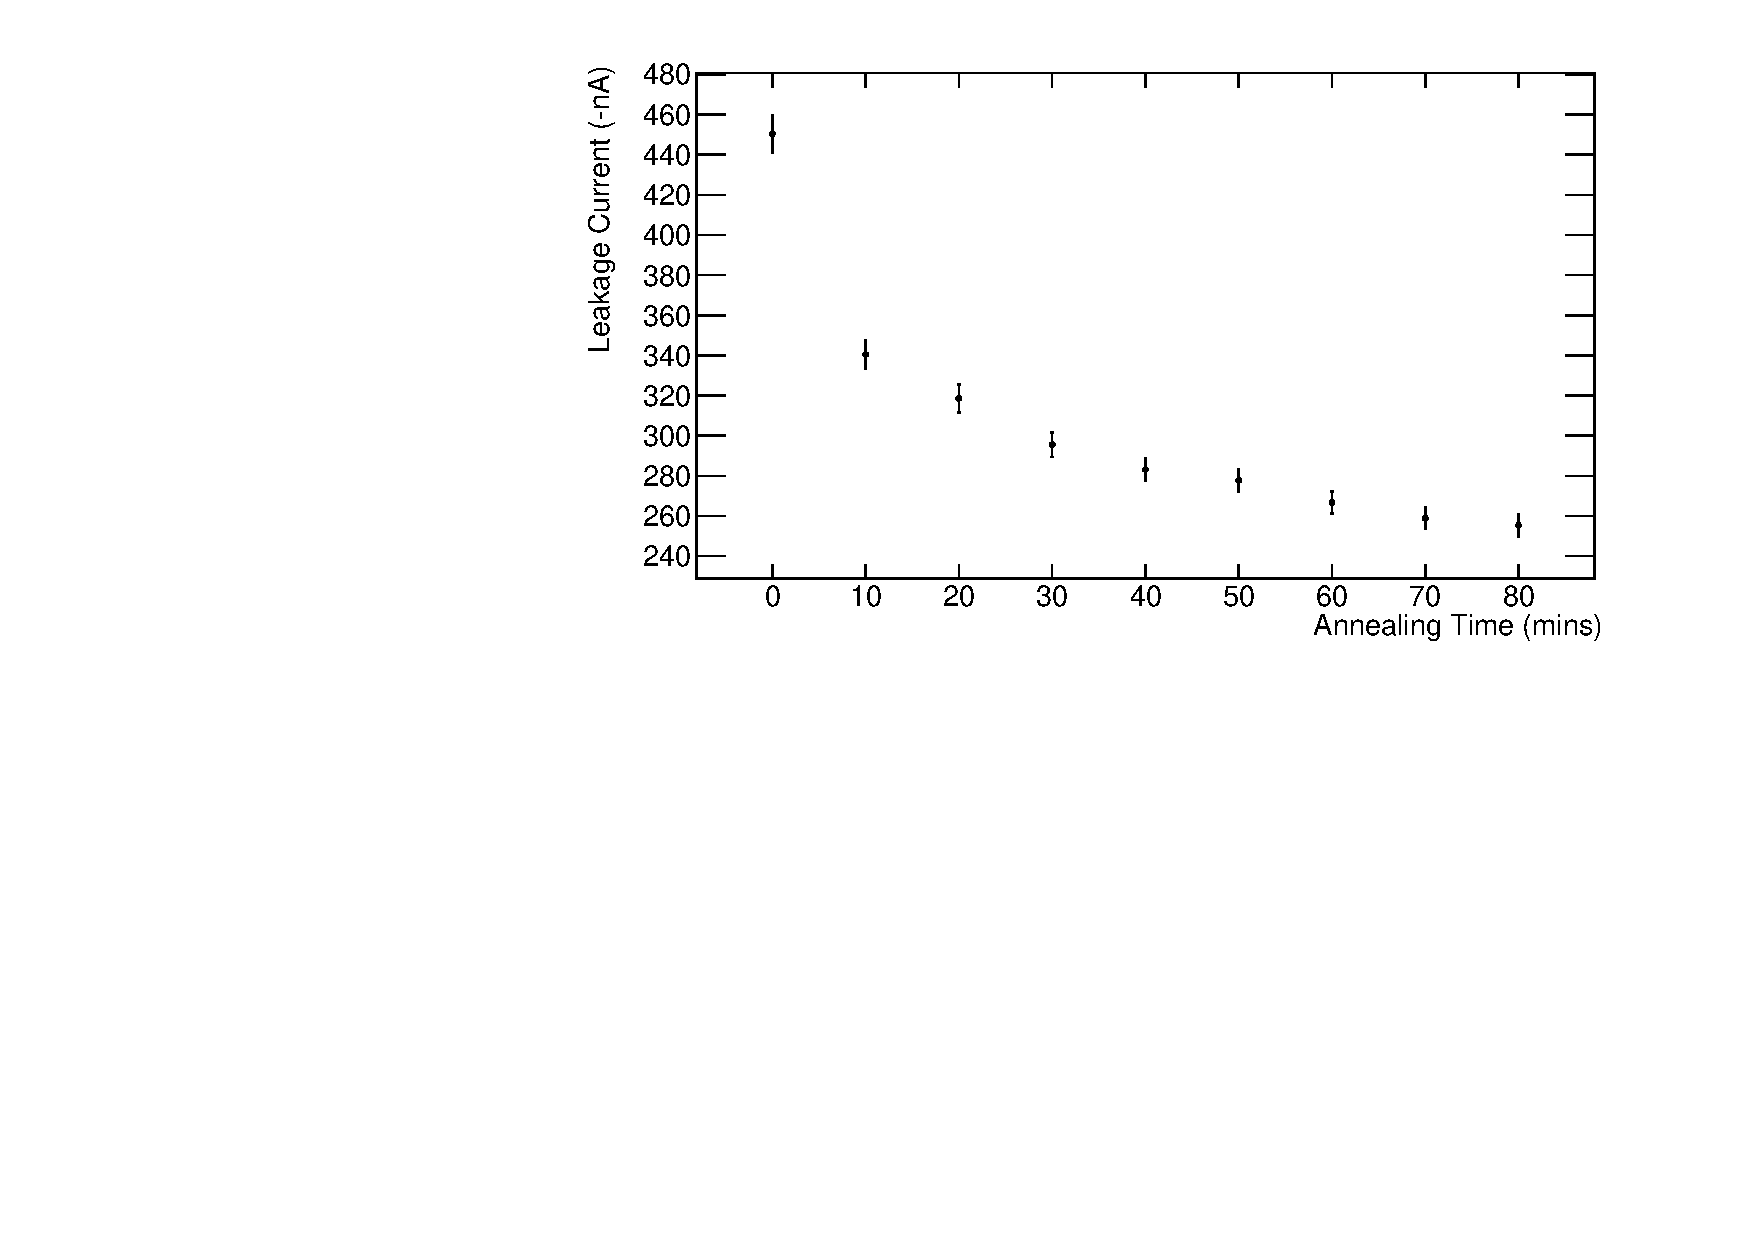
\includegraphics[width = 0.8\linewidth]{Diode5_annealing_10min_increments_2411.pdf}
            \caption{\scriptsize Change in leakage current due to annealing}
        \end{figure}
        \vspace{-0.5cm}
        After \textbf{80 minutes of annealing at $\bm{60^{\circ}}$C}, it can be seen that any thermal history has effectively been removed.
    \end{frame}
    
    \begin{frame}{Annealing}{The Effect on Leakage Current}
        \begin{figure}
            \centering
            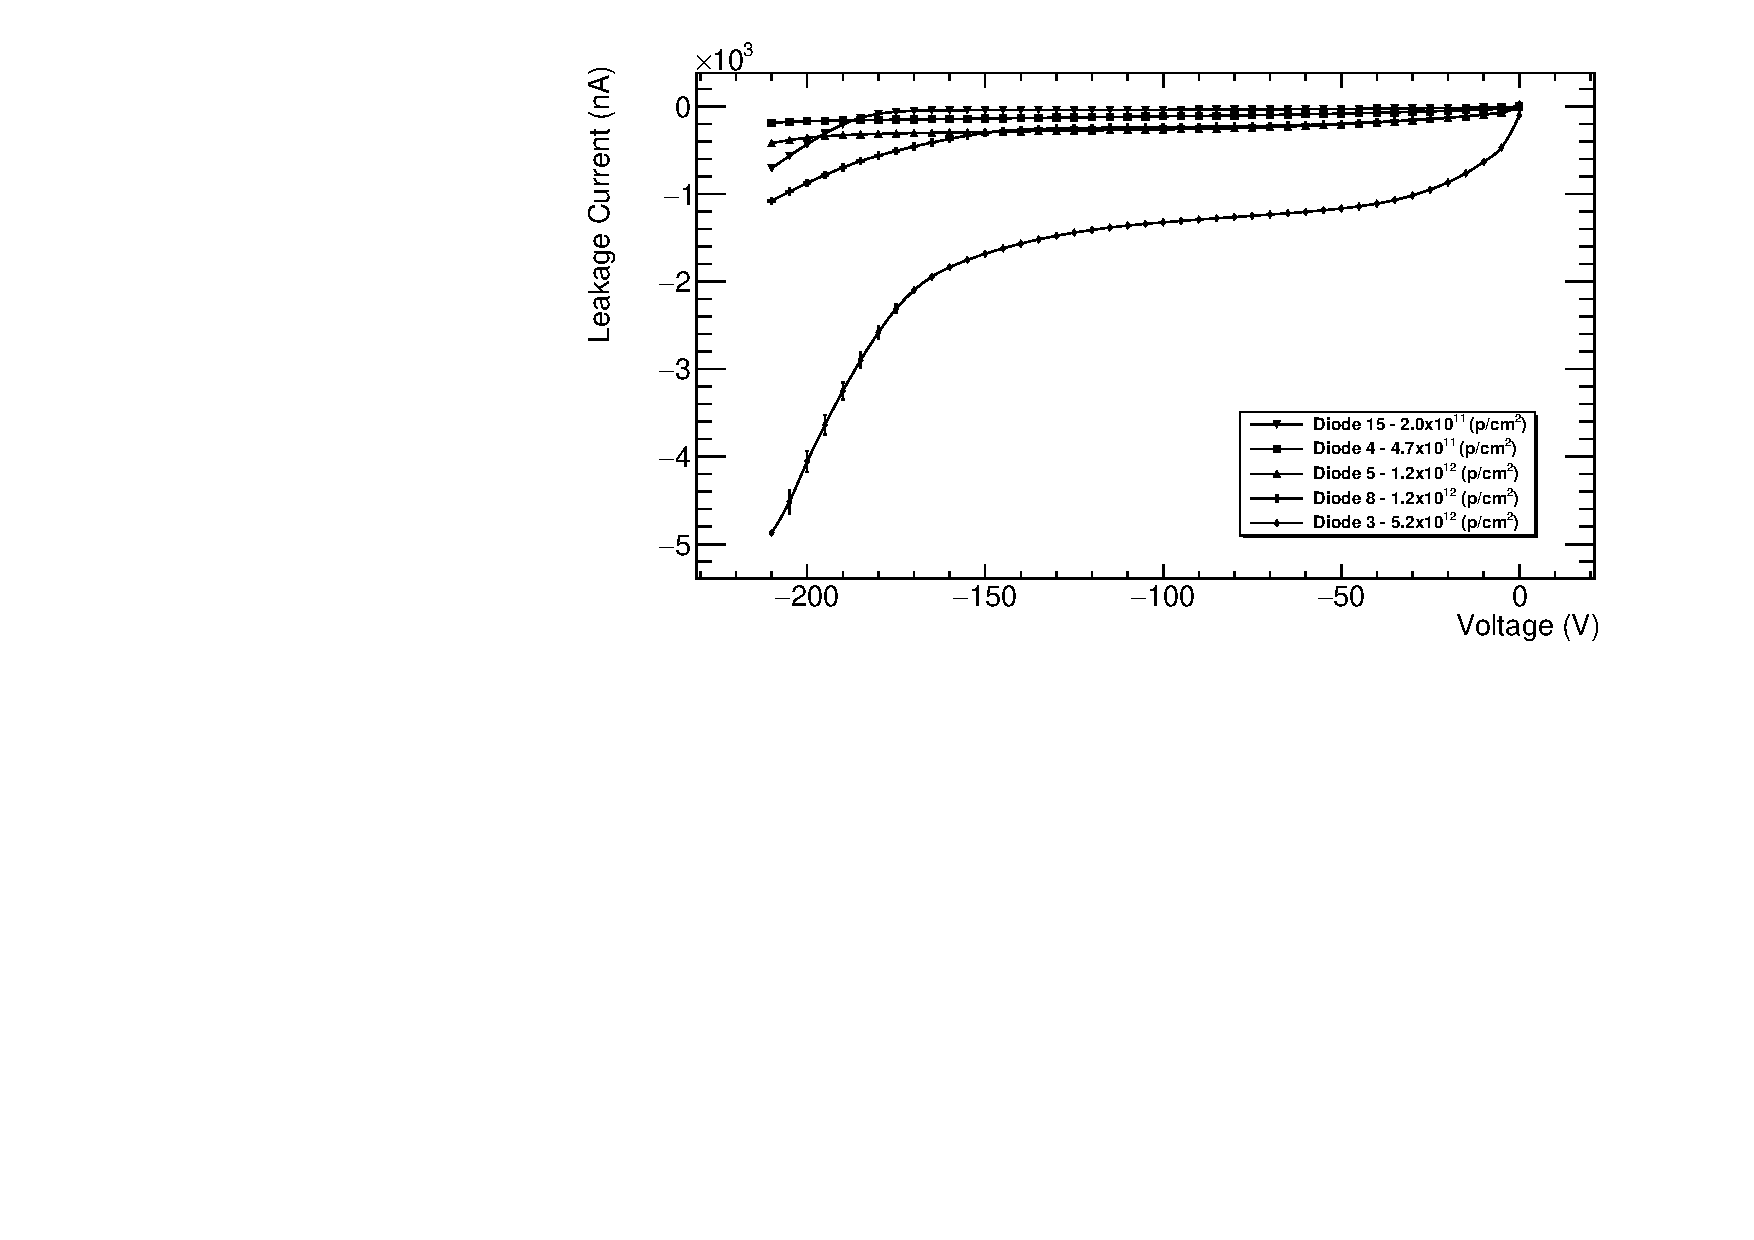
\includegraphics[width = 0.95\linewidth]{MultiDiode_Anneal_Fluence_0512.pdf}
            \caption{Leakage current changes after irradiations and annealing.}
        \end{figure}
    \end{frame}
    
\section{Determining the Hardness Factor}
    
    \begin{frame}{Determining the Hardness Factor}{Leakage Current Variation with Fluence}
        \begin{itemize}
            \item The \textbf{change in leakage current} before and after irradiation is related to \textbf{proton fluence} by \textsuperscript{\cite{Moll}}:
                \begin{equation*}
                    \Delta I = \alpha L^2 w \phi
                \end{equation*}
            \item The \textbf{hardness factor} can be written as:
                \begin{equation*}
                    \kappa = \frac{\alpha}{\alpha _{neq}}\hspace{0.5cm}\text{since}\hspace{0.5cm}\kappa = \frac{\phi _{neq}}{\phi}
                \end{equation*}
                Where $\alpha _{neq} = (3.99 \pm 0.03)\times 10^{-17}$ Acm\textsuperscript{-1} \textsuperscript{\cite{Moll}}.
            \item Therefore, \textbf{plotting change in leakage current vs fluence} should give a straight line graph with $\bm{\alpha L^2w}$ as the gradient.
        \end{itemize}
    \end{frame}

\subsection{Results for MC40 Cyclotron}

    \begin{frame}{Determining the Hardness Factor}{Results for MC40 Cyclotron}
        \begin{figure}
            \centering
            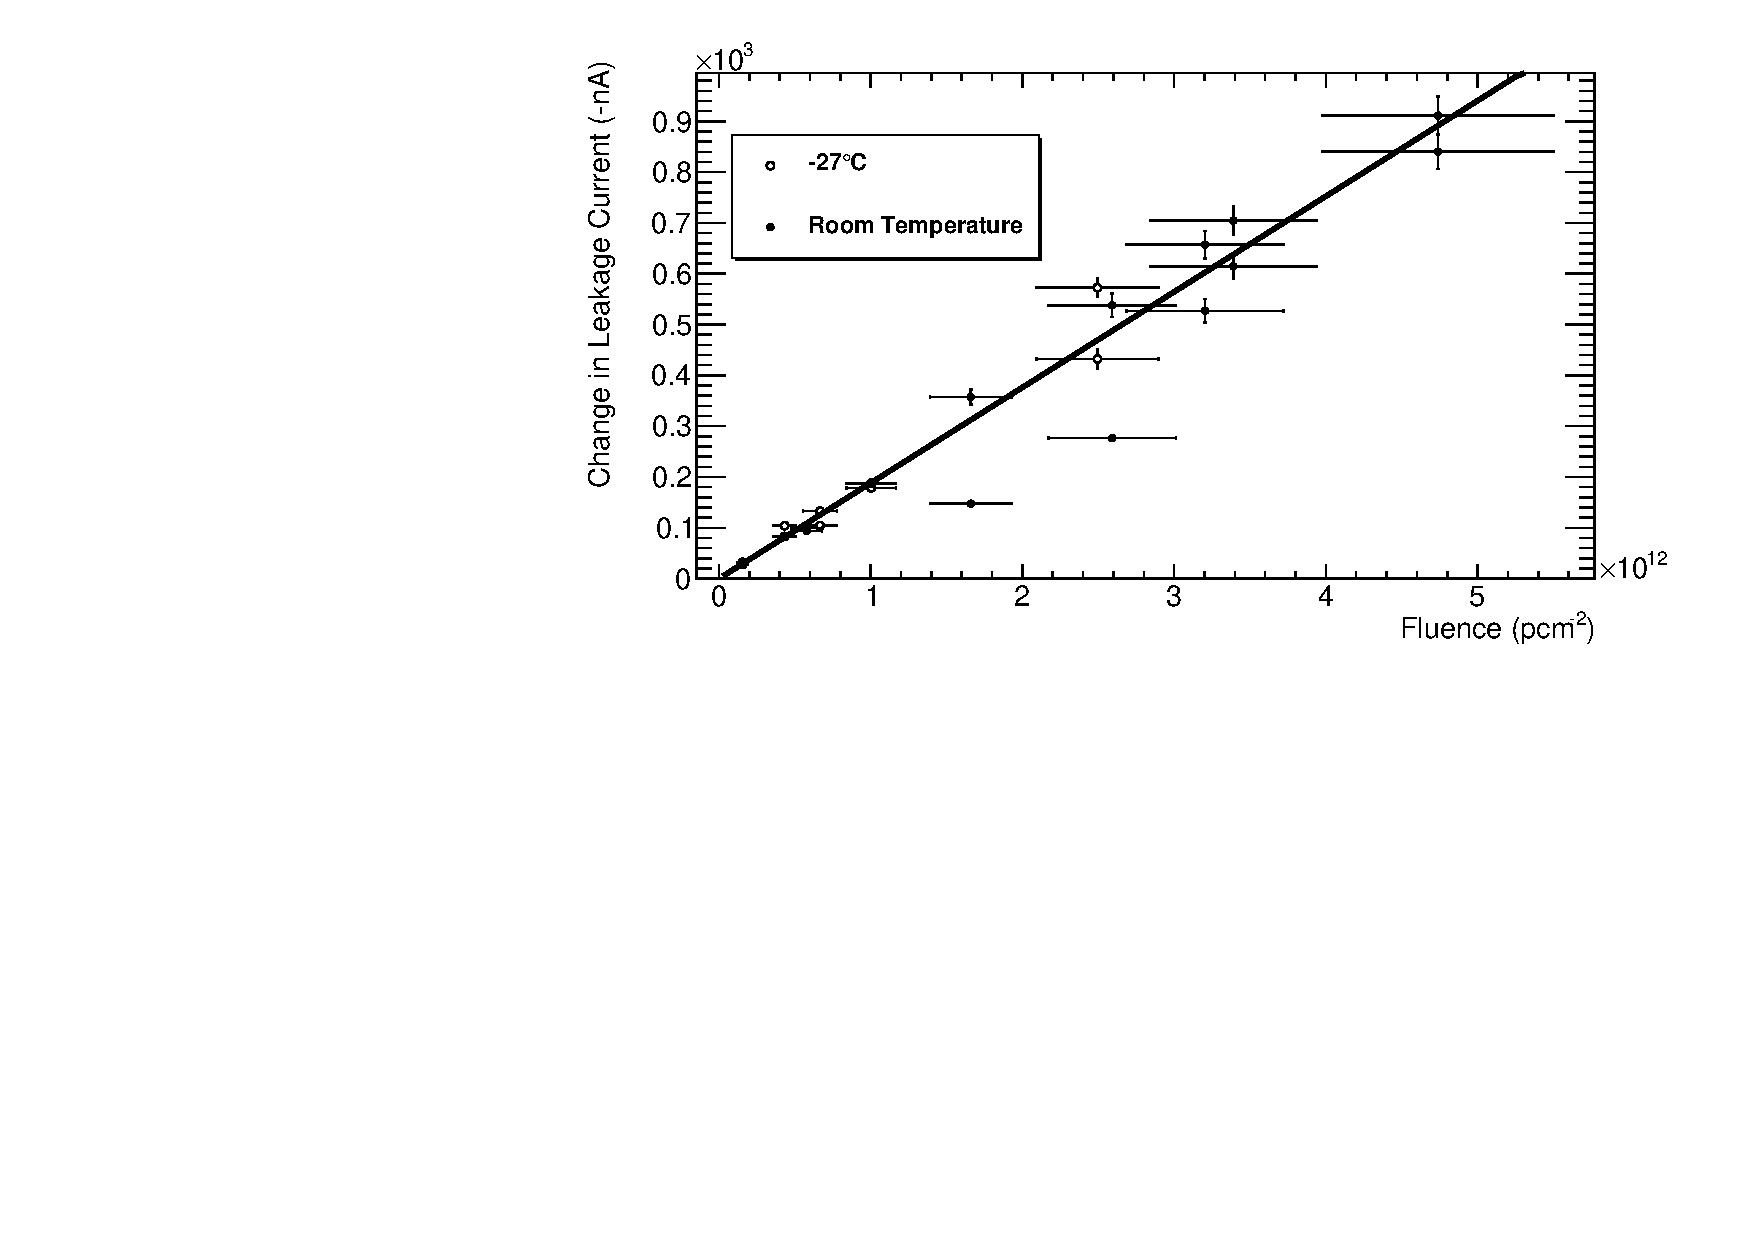
\includegraphics[width = 0.85\linewidth]{HardnessFactor_FinalResult_1Fit_0603.pdf}
            \caption{Change in leakage current vs proton fluence.}
        \end{figure}
        \vspace{-0.5cm}
        This gave a combined value of $\alpha = (8.93\pm 0.34)\times 10^{-17}$ Acm\textsuperscript{-1}. Hence, the hardness factor was found to be:
            \begin{equation*}
                \boxed{\kappa _{MC40} = 2.24\pm 0.09}
            \end{equation*}
    \end{frame}
    
\subsection{Results for KIT}
    
    \begin{frame}{Determining the Hardness Factor}{Results for KIT}
        \vspace{-0.8cm}
        \begin{figure}
            \centering
            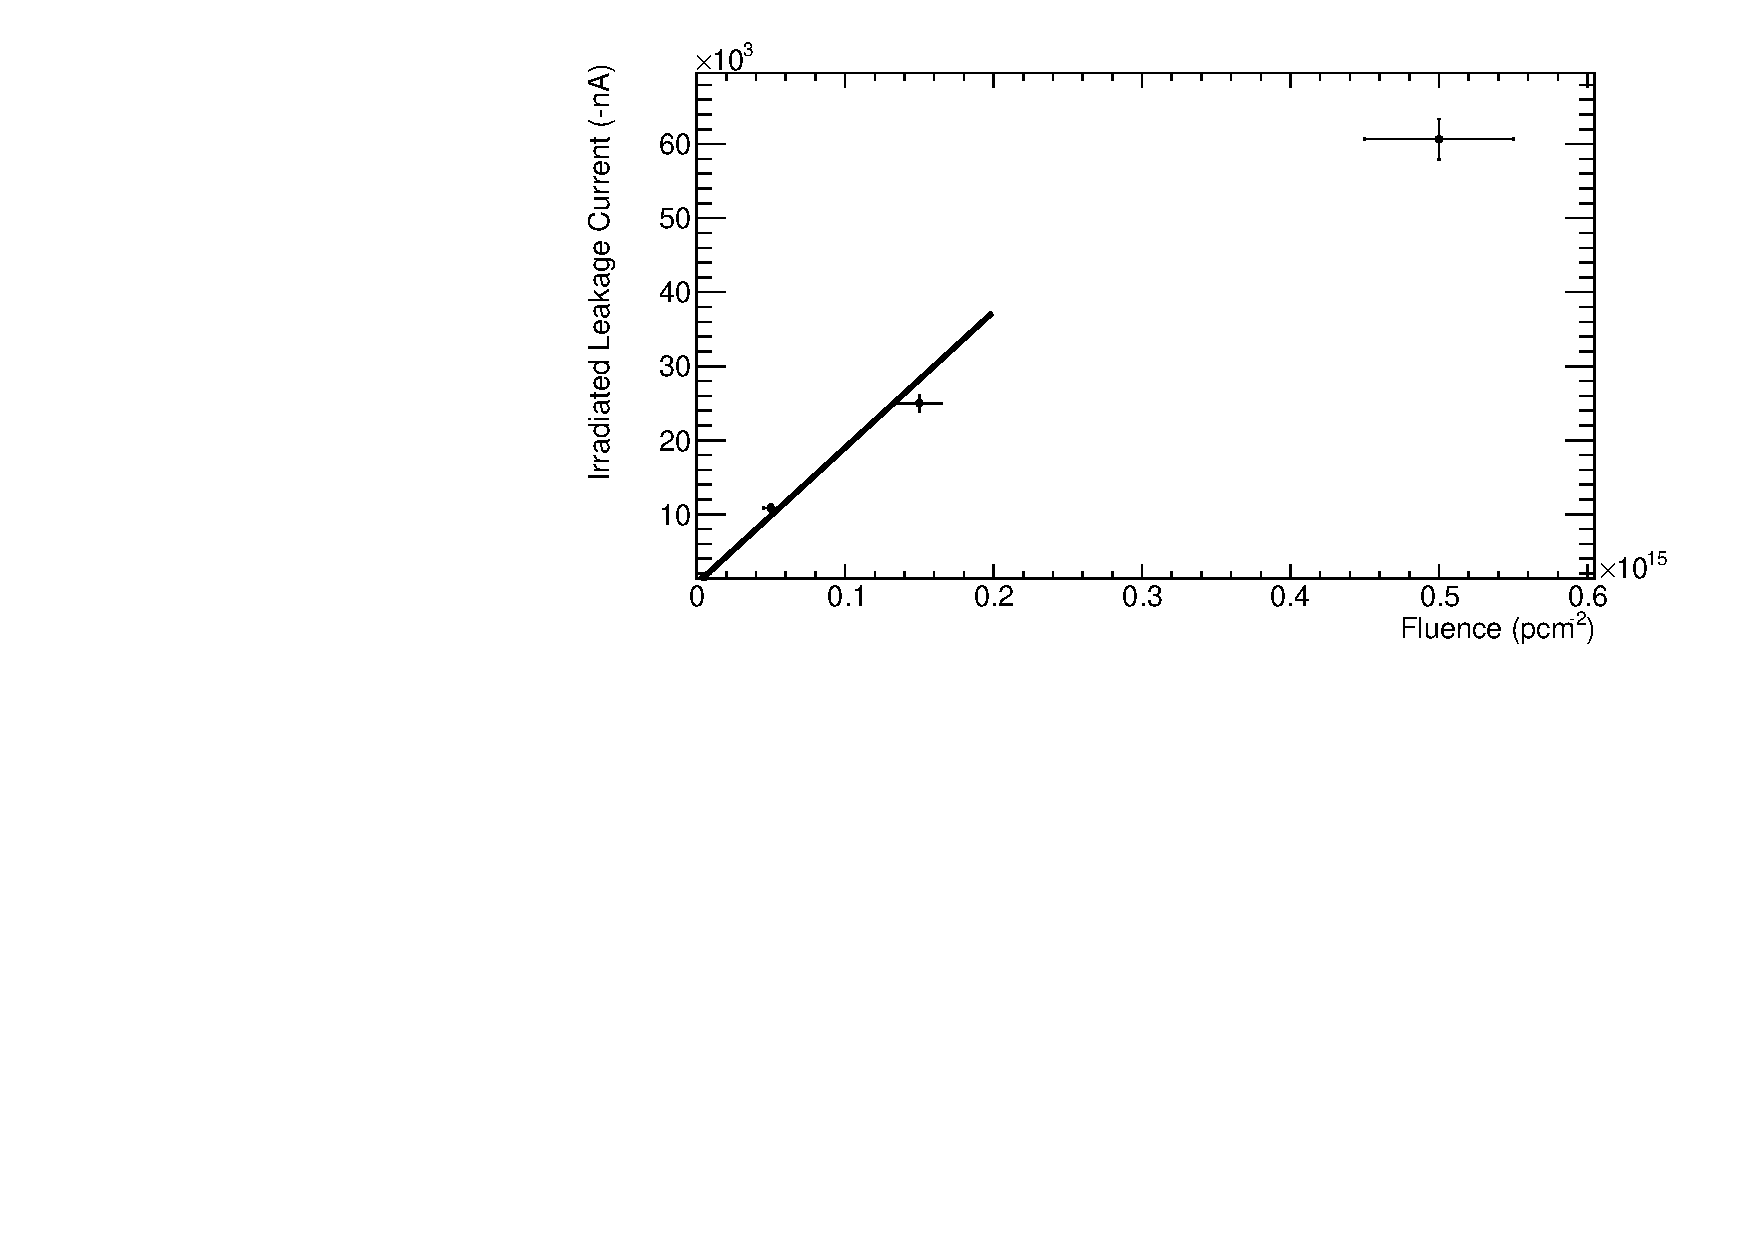
\includegraphics[width = 0.8\linewidth, trim = {0 0 0 0cm}, clip = true]{KIT_deltaI_fluence_2302.pdf}
            \vspace{-0.4cm}
            \caption{\scriptsize Irradiated leakage current vs proton fluence for KIT photodiodes.}
        \end{figure}
        \vspace{-0.65cm}
        This gave a value of $\alpha = (8.77\pm 1.06)\times 10^{-17}$ Acm\textsuperscript{-1}. Hence, the hardness factor for KIT was found to be:
        \vspace{-0.3cm}
            \begin{equation*}
                \boxed{\kappa _{KIT} = 2.20\pm 0.27}
            \end{equation*}
        \vspace{-0.1cm}
        Which is in agreement with our result, and the quoted value of $2.05 \pm 0.61$.
    \end{frame}

\section{Summary}
    
    \begin{frame}{Summary}
        \begin{itemize}
            \item The \textbf{I--V} and \textbf{C--V} characteristics of \textbf{BPW34F photodiodes} have been analysed.
            \vspace{0.5cm}
            \item Using this, we have obtained a value of $\bm{\kappa _{MC40} = 2.24\pm 0.09}$ for the MC40 Cyclotron.
            \vspace{0.5cm}
            \item Applying the same method to photodiodes from \textbf{KIT}, a value of $\bm{\kappa _{KIT} = 2.20\pm 0.27}$ was obtained.
            \vspace{0.5cm}
            \item Our value \textbf{agrees} with the value obtained from \textbf{KIT} photodiodes.
        \end{itemize}
    \end{frame}
    
    \begin{frame}{References}
        \printbibliography
    \end{frame}
    
    \begin{frame}{Appendix: I--V Measurements}{Calculating the Activation Energy}
        \begin{figure}
            \centering
            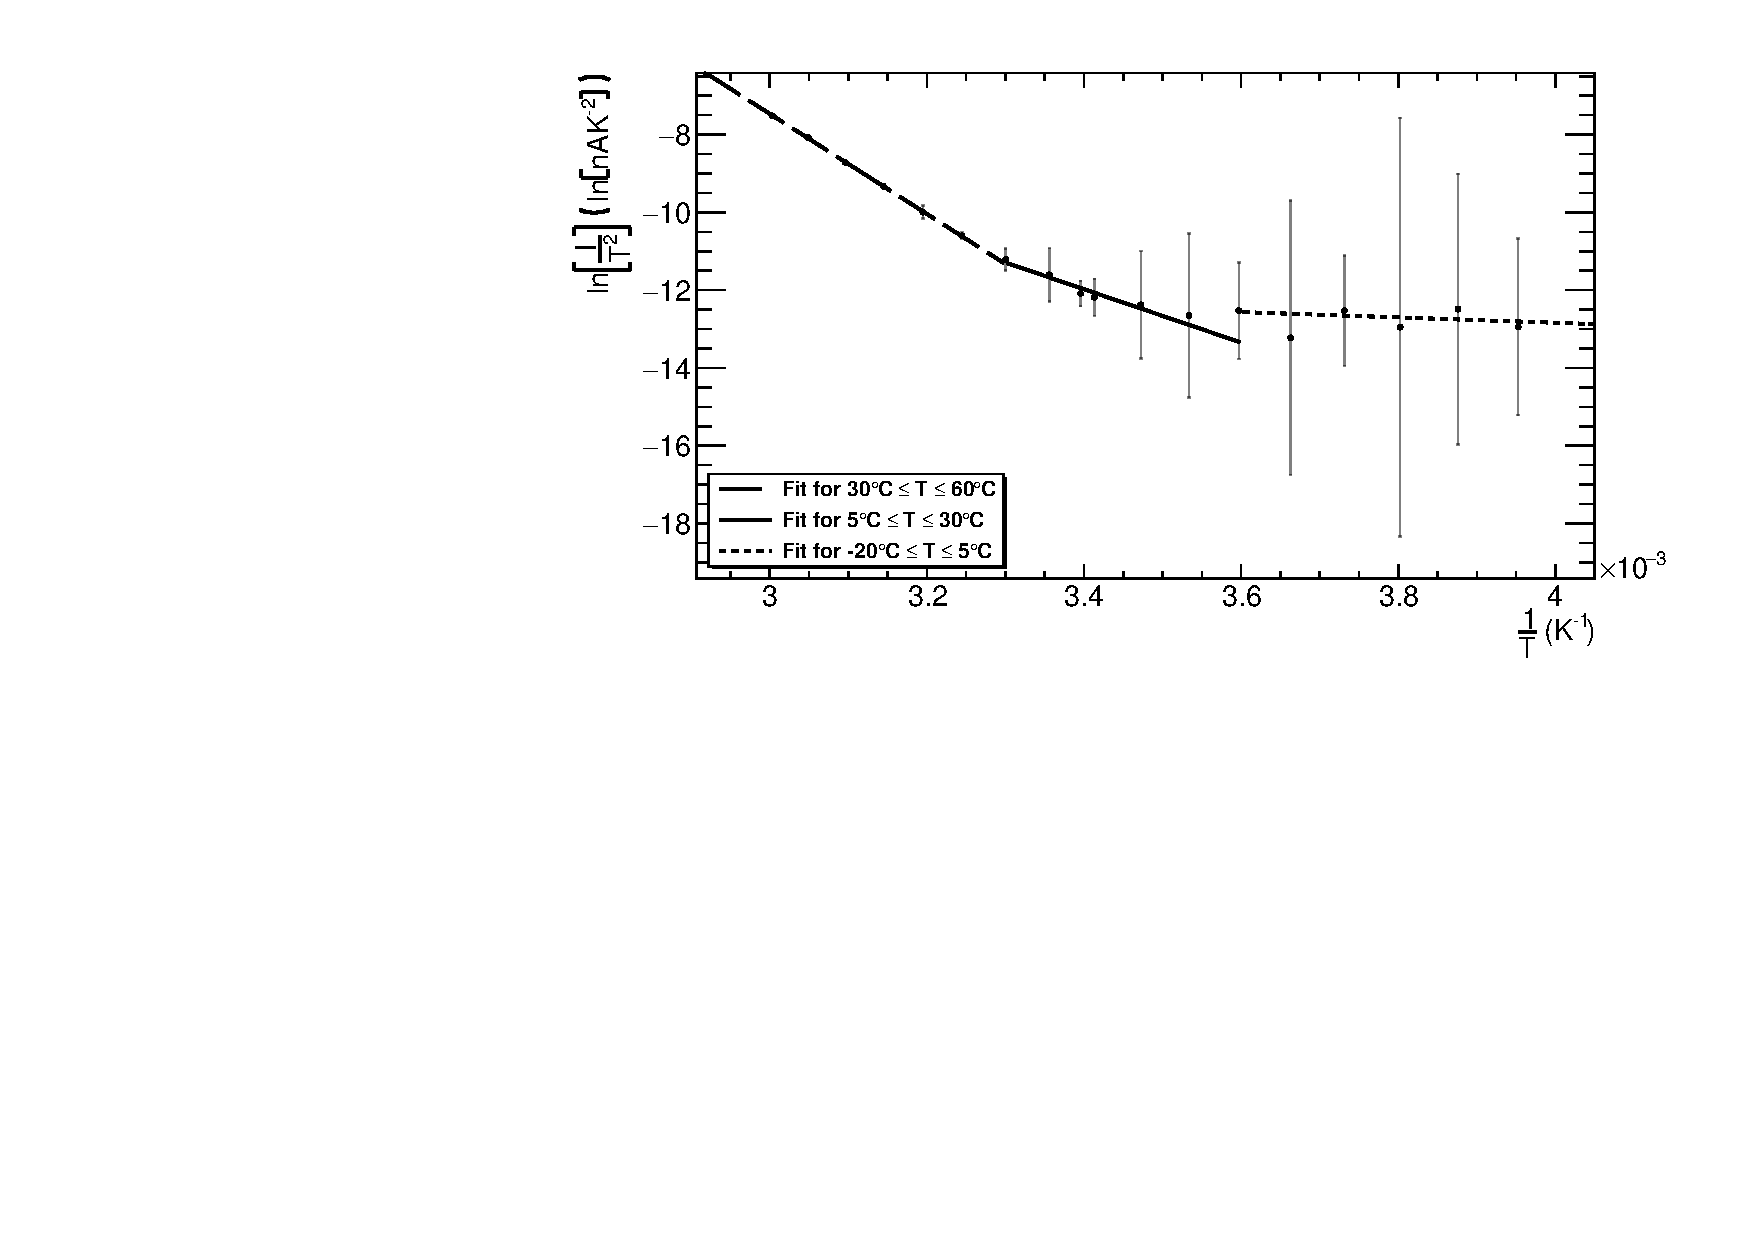
\includegraphics[width = 0.8\linewidth]{BandGap_fullrange_BlackandWhite_3101.pdf}
            \caption{$\ln \left[{\frac{I}{T^2}}\right]$ vs $\frac{1}{T}$. The leakage current is evaluated at maximum depletion.}
            \label{fig:BandGapFull}
        \end{figure}
        \vspace{-0.5cm}
        \begin{equation*}
            \ln \left[{\frac{I}{T^2}}\right] = -\frac{E_a}{2k_B}\frac{1}{T}
        \end{equation*}
    \end{frame}
    
    \begin{frame}{Appendix: I--V Measurements}{Calculating the Activation Energy}
        {\small $E_a^{high} = 2.22 \pm 0.03$ eV; $E_a^{mid} = 1.18 \pm 0.50$ eV; $E_a^{low} = 0.12 \pm 1.84$ eV.}
        \vspace{0.5cm}
        \begin{itemize}   
            \item The accepted value is $\bm{E_a^{accepted} = 1.21}$ \textbf{eV} \textsuperscript{\cite{BandGap}}.
            \vspace{0.5cm}
            \item $E_a^{low}$ is unreliable since the \textbf{noise floor} of the Keithley becomes a problem at lower temperatures.
        \end{itemize}
    \end{frame}
    
    \begin{frame}{Appendix: C--V Measurements}{AC Frequency Dependence}
        \begin{itemize}
            \item For \textbf{radiation damaged} photodiodes, the AC frequency applied to the system will have an affect on capacitance.
            \item As higher frequencies are reached, varying modes of radiation damage will activate.
        \end{itemize}
        \begin{figure}
            \centering
            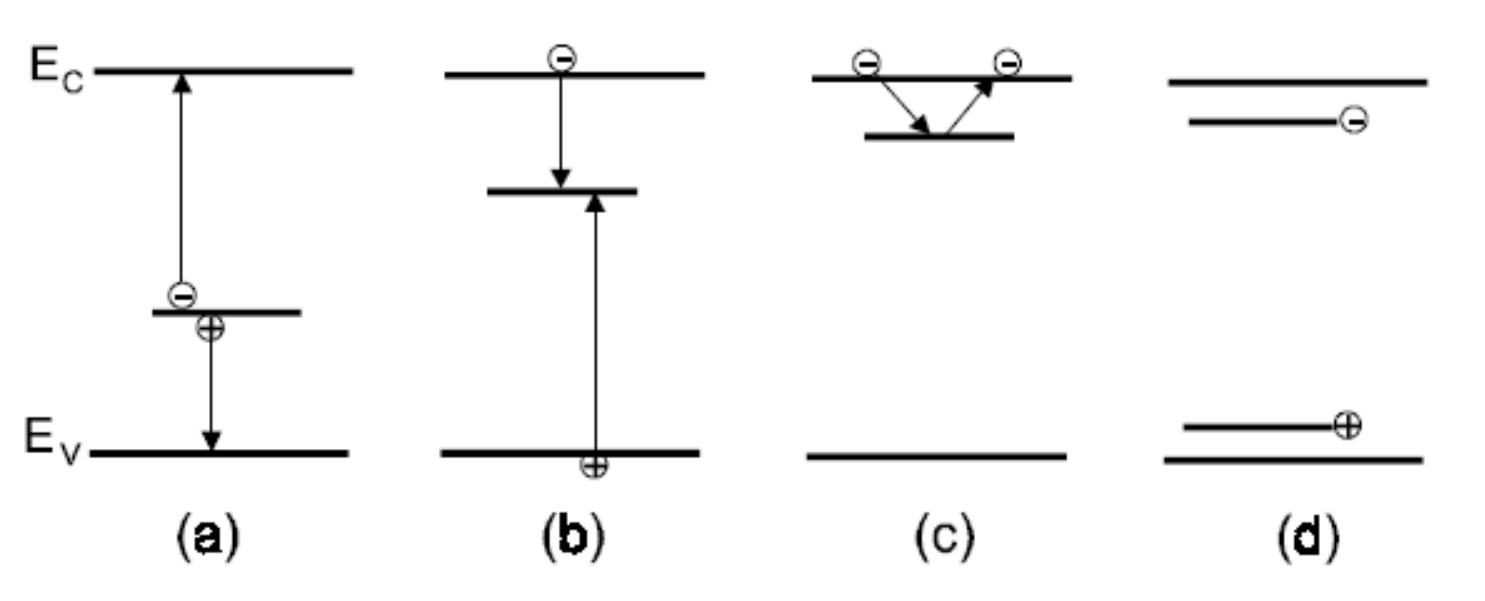
\includegraphics[width = 0.8\linewidth]{DefectEnergyLevels.png}
            \caption{Radiation damage processes: (a) generation, (b) recombination, (c) trapping, (d) compensation \textsuperscript{\cite{Casse}}.}
            \label{fig:damageprocesses}
        \end{figure}
    \end{frame}
    
    \begin{frame}{Appendix: C--V Measurements}{AC Frequency Dependence}
        \begin{figure}
            \centering
            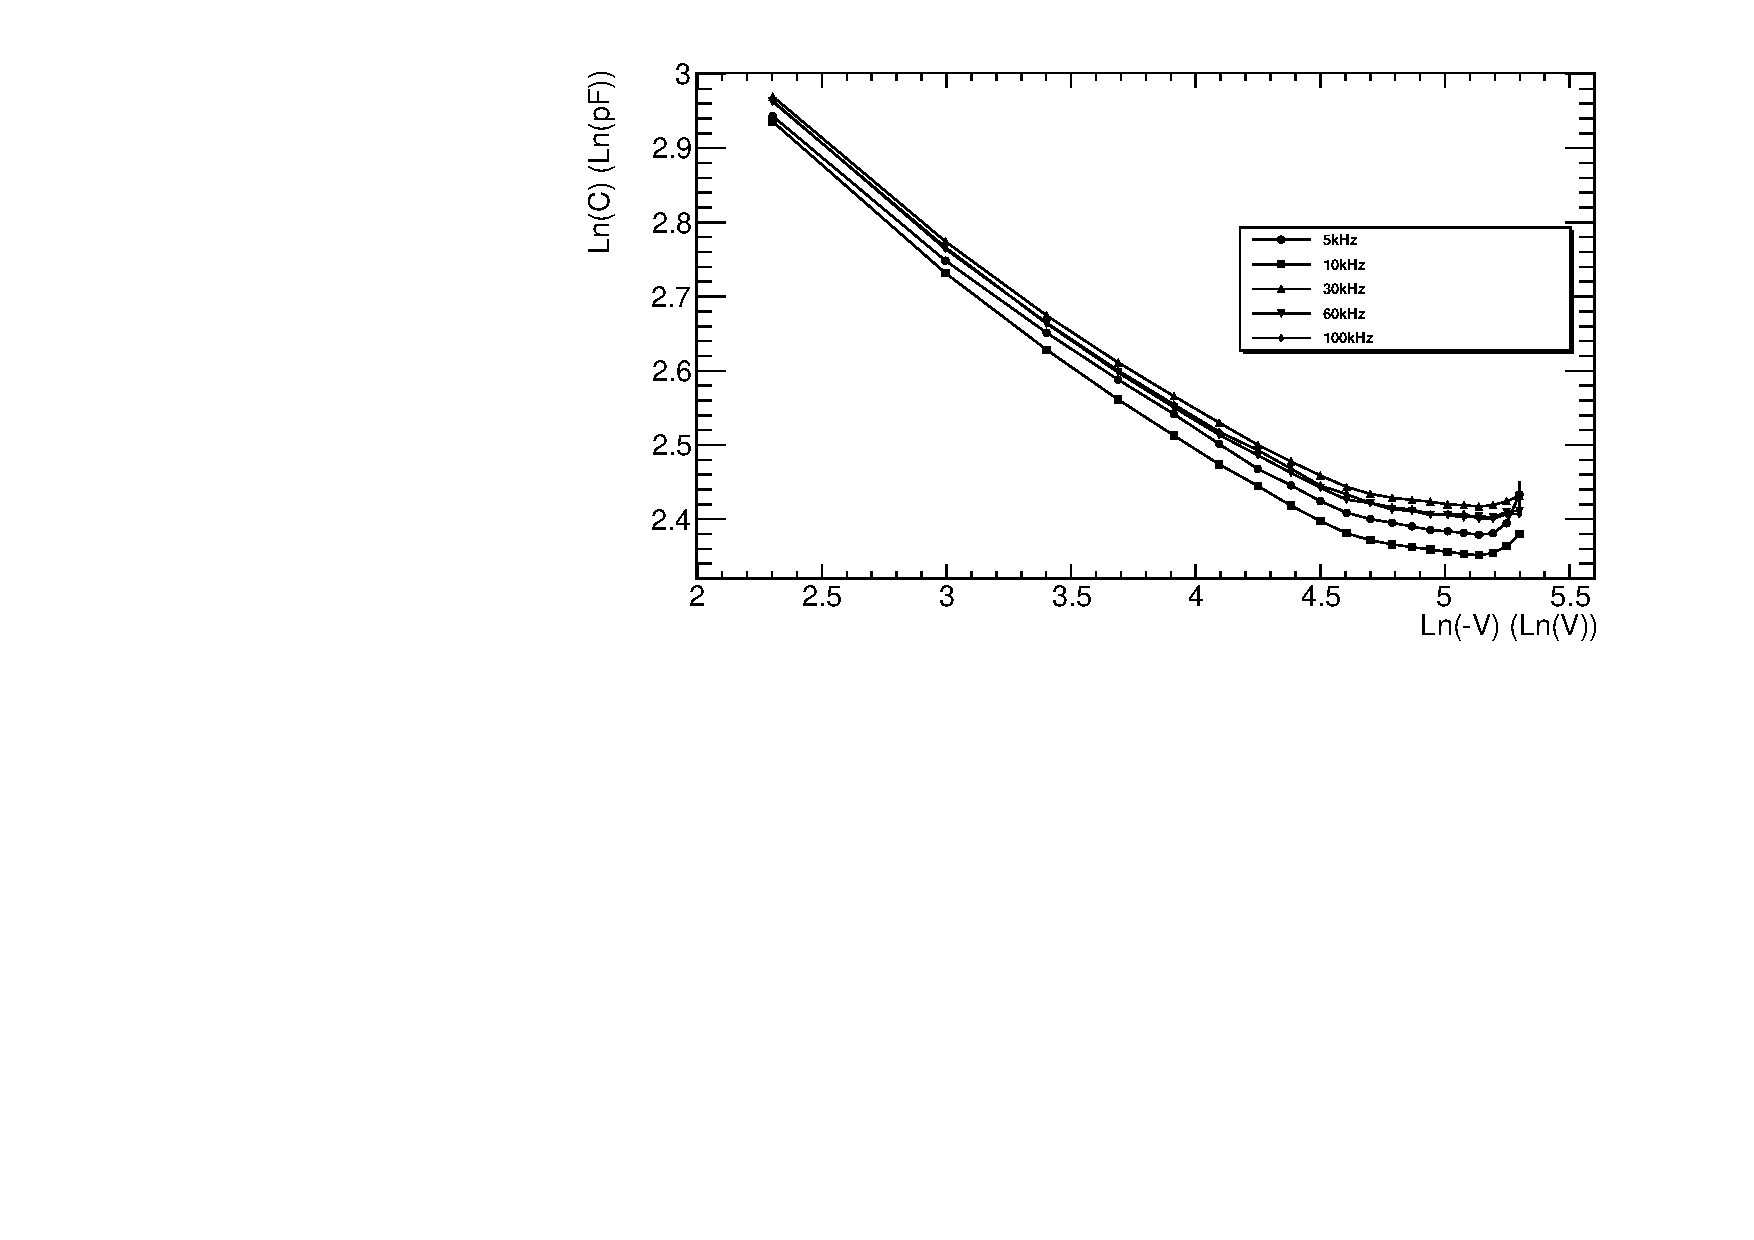
\includegraphics[width = 0.9\linewidth]{Diode24_nonirradiated_CV_frequency_2301.pdf}
            \caption{AC frequency effect on capacitance (non-irradiated).}
            \label{fig:freqcvnonirradiated}
        \end{figure}
    \end{frame}
    
    \begin{frame}{Appendix: C--V Measurements}{AC Frequency Dependence}
        \begin{figure}
            \centering
            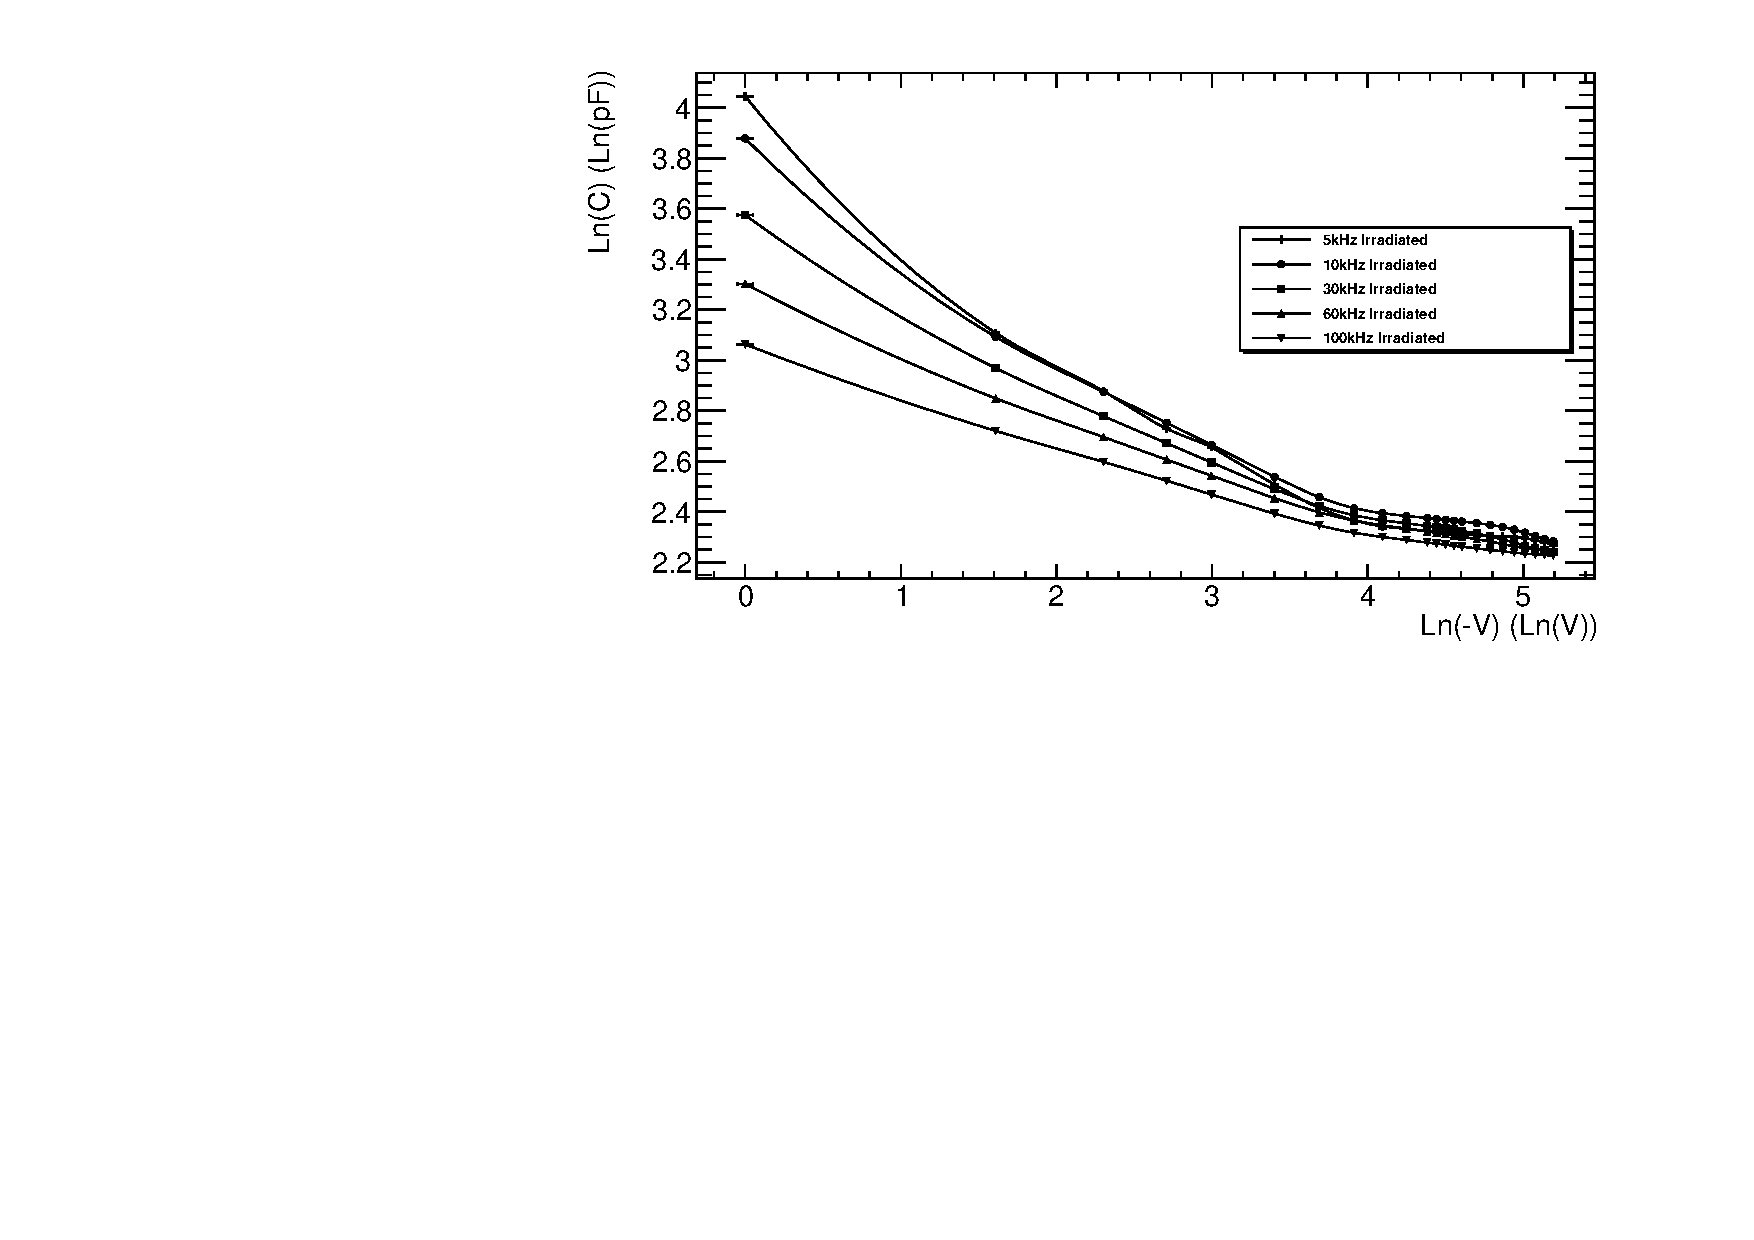
\includegraphics[width = 0.9\linewidth]{Diode3_CV_0802_prettygraph.pdf}
            \caption{AC frequency effect on capacitance (irradiated).}
            \label{fig:freqcvirradiated}
        \end{figure}
    \end{frame}
    
    \begin{frame}{Appendix: C--V Measurements}{Fluence Dependence of Maximum Depletion Voltage.}
        \begin{itemize}
            \item During C--V measurements on an irradiated photodiode, it was found that the \textbf{maximum depletion voltage depends upon the degree of radiation damage}.
        \end{itemize}
        \begin{figure}
            \centering
            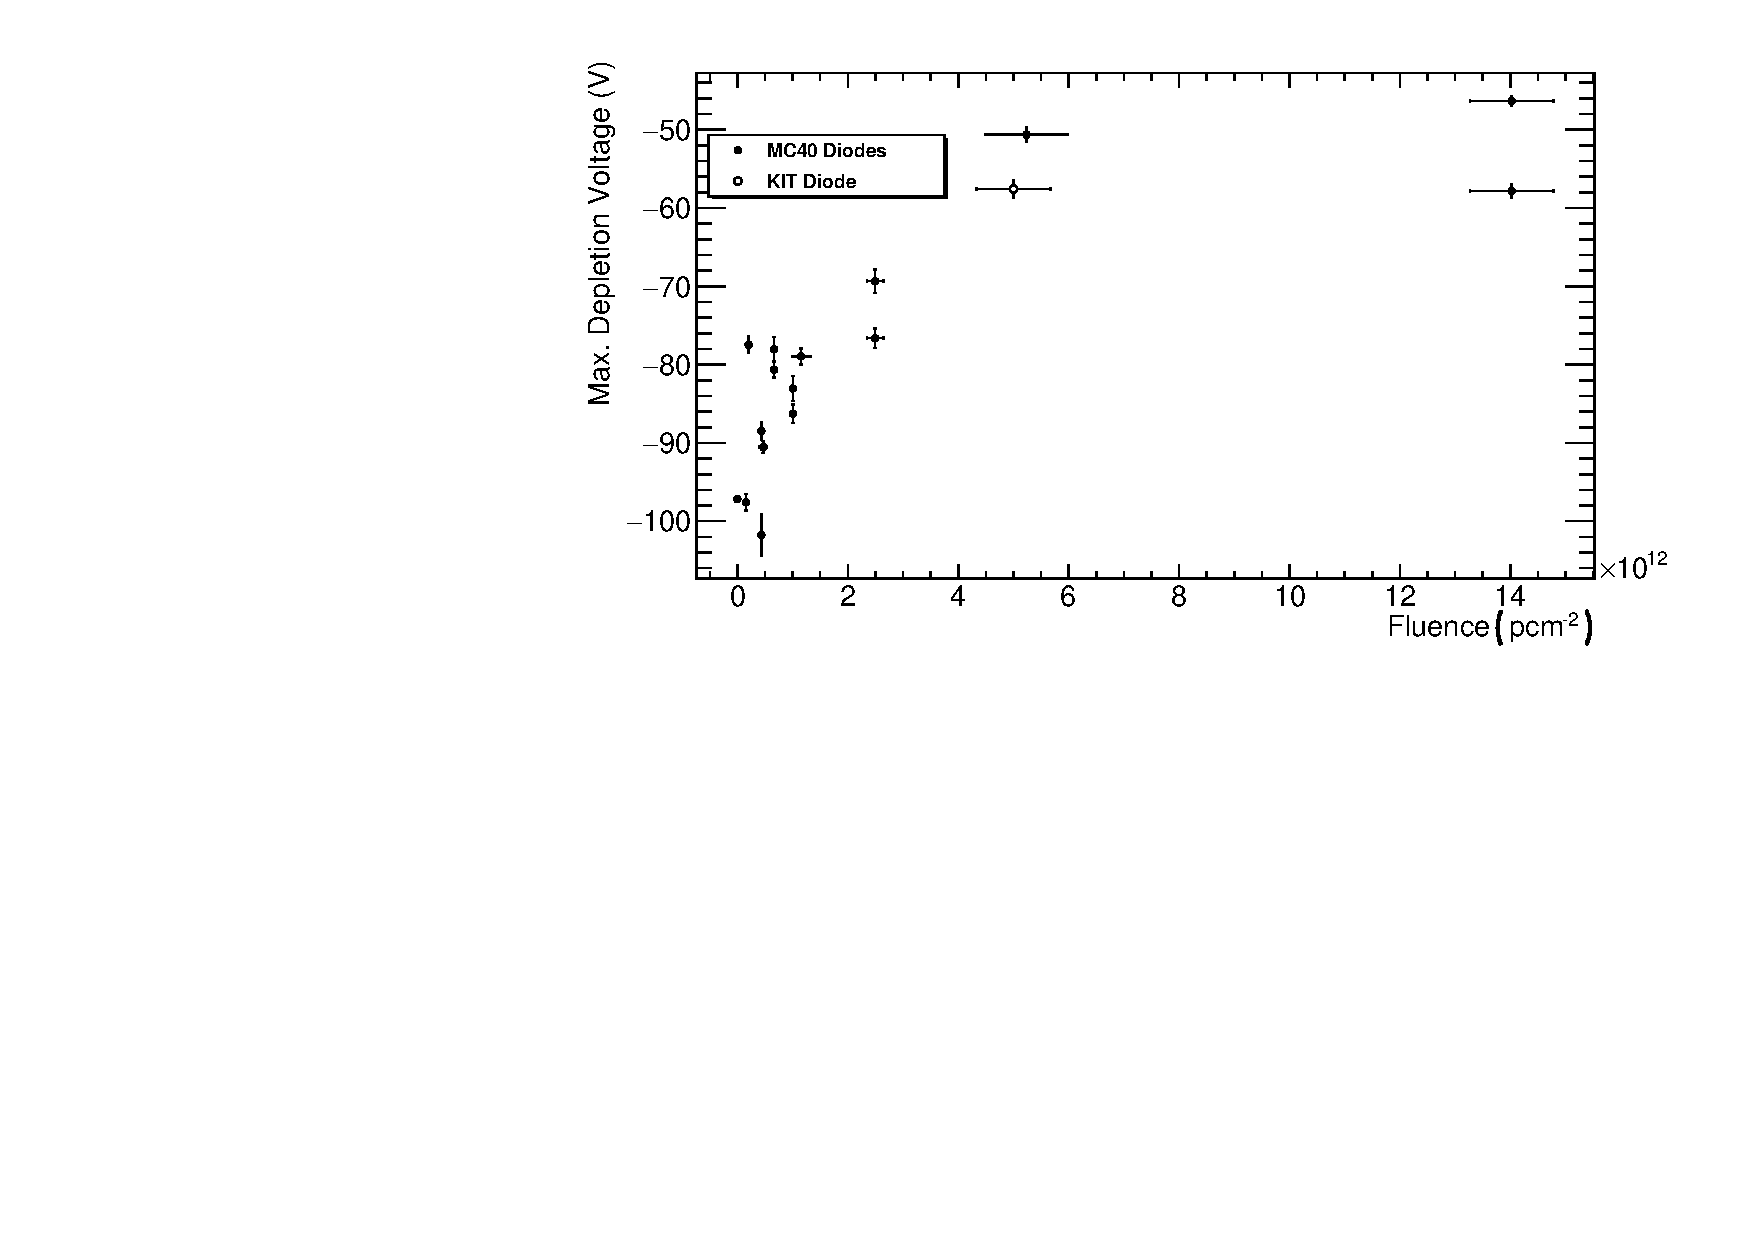
\includegraphics[width = 0.9\linewidth]{MaxDepletion_vs_fluence_alldata_0503.pdf}
            \vspace{-0.3cm}
            \caption{Maximum depletion voltage as a function of fluence.}
            \label{fig:maxdepletionfluence}
        \end{figure}
    \end{frame}
    
    \begin{frame}{Appendix: Determining the Hardness Factor}{Room Temperature Data}
        \begin{figure}
            \centering
            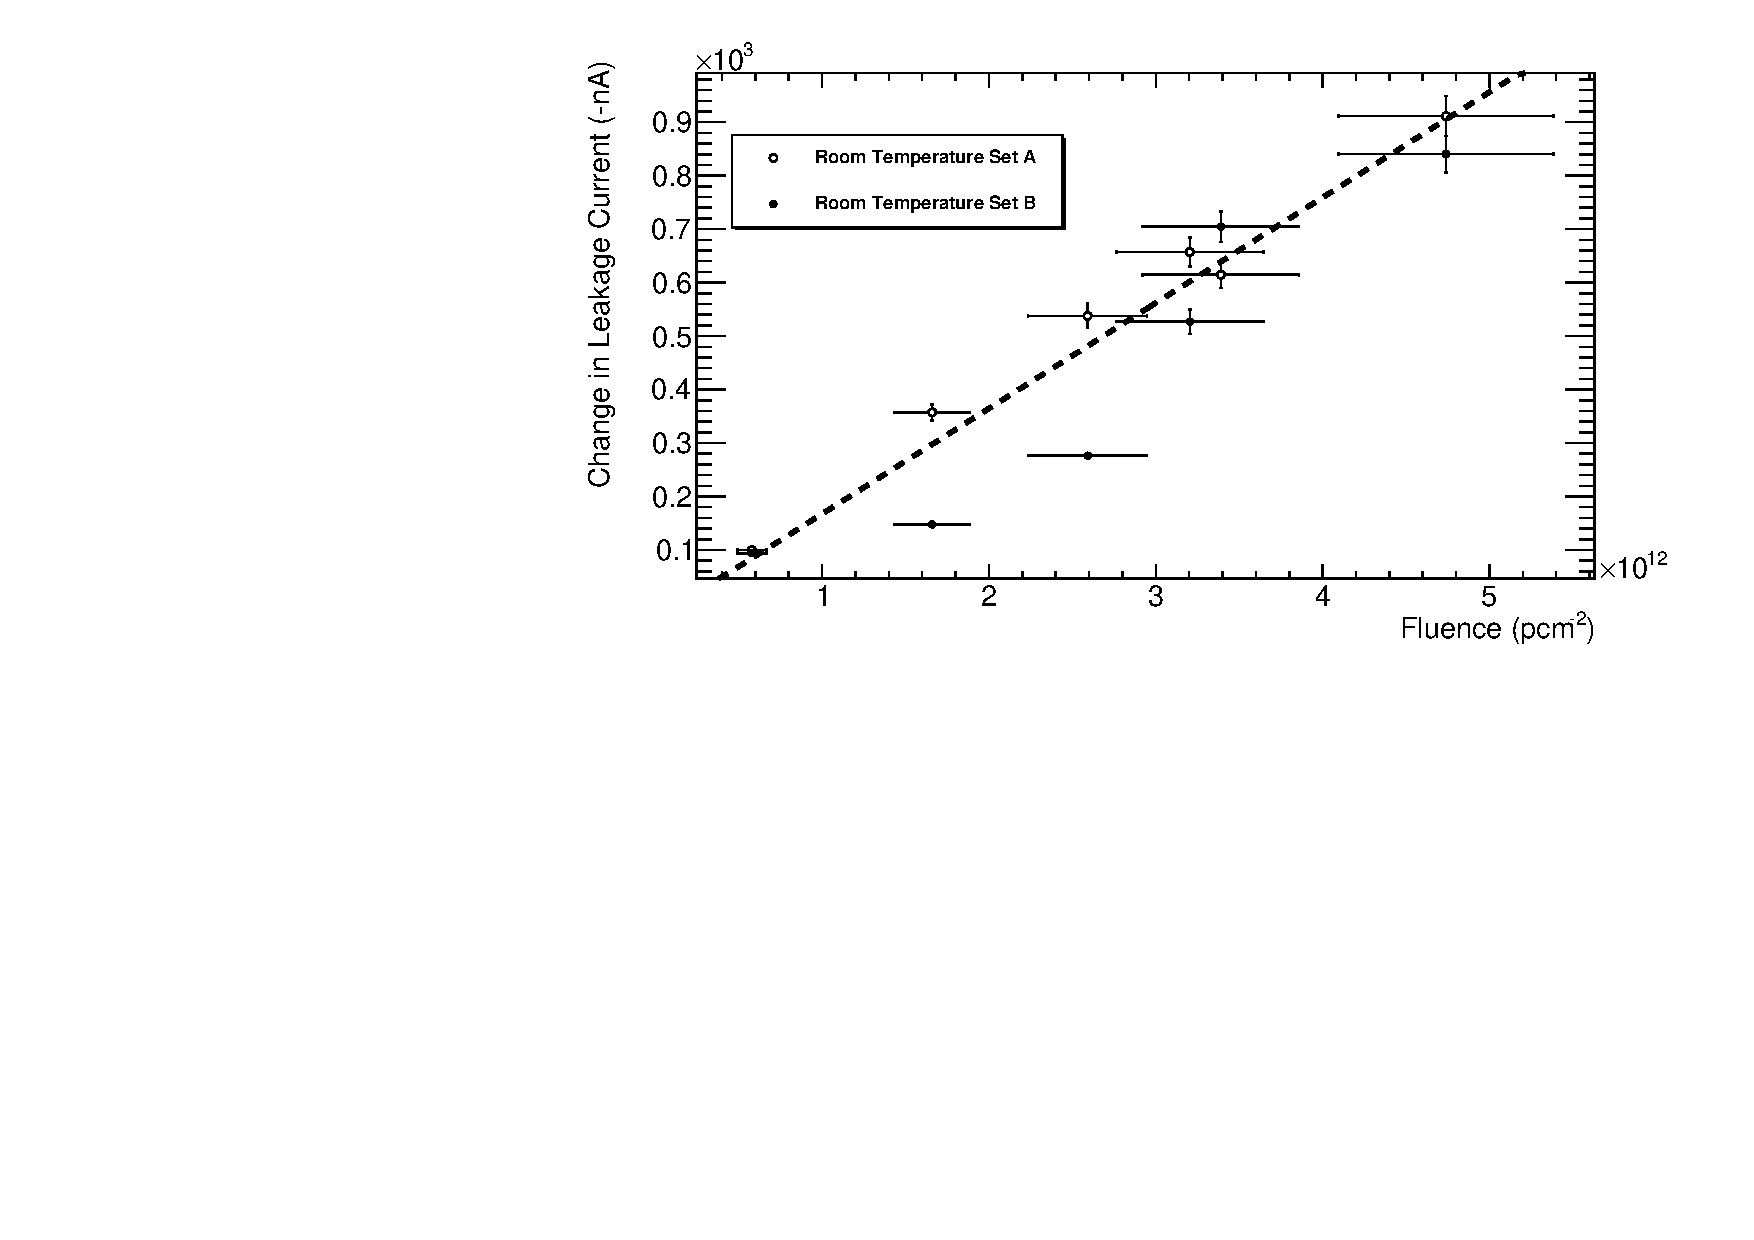
\includegraphics[width=0.9\linewidth]{Leakage_Fluence_Combined_Warm_0603.pdf}
            \caption{Change in leakage current vs proton fluence for room temperature data.}
        \end{figure}
    \end{frame}
    
    \begin{frame}{Appendix: Determining the Hardness Factor}{$-27^{\circ}$C Temperature Data}
        \begin{figure}
            \centering
            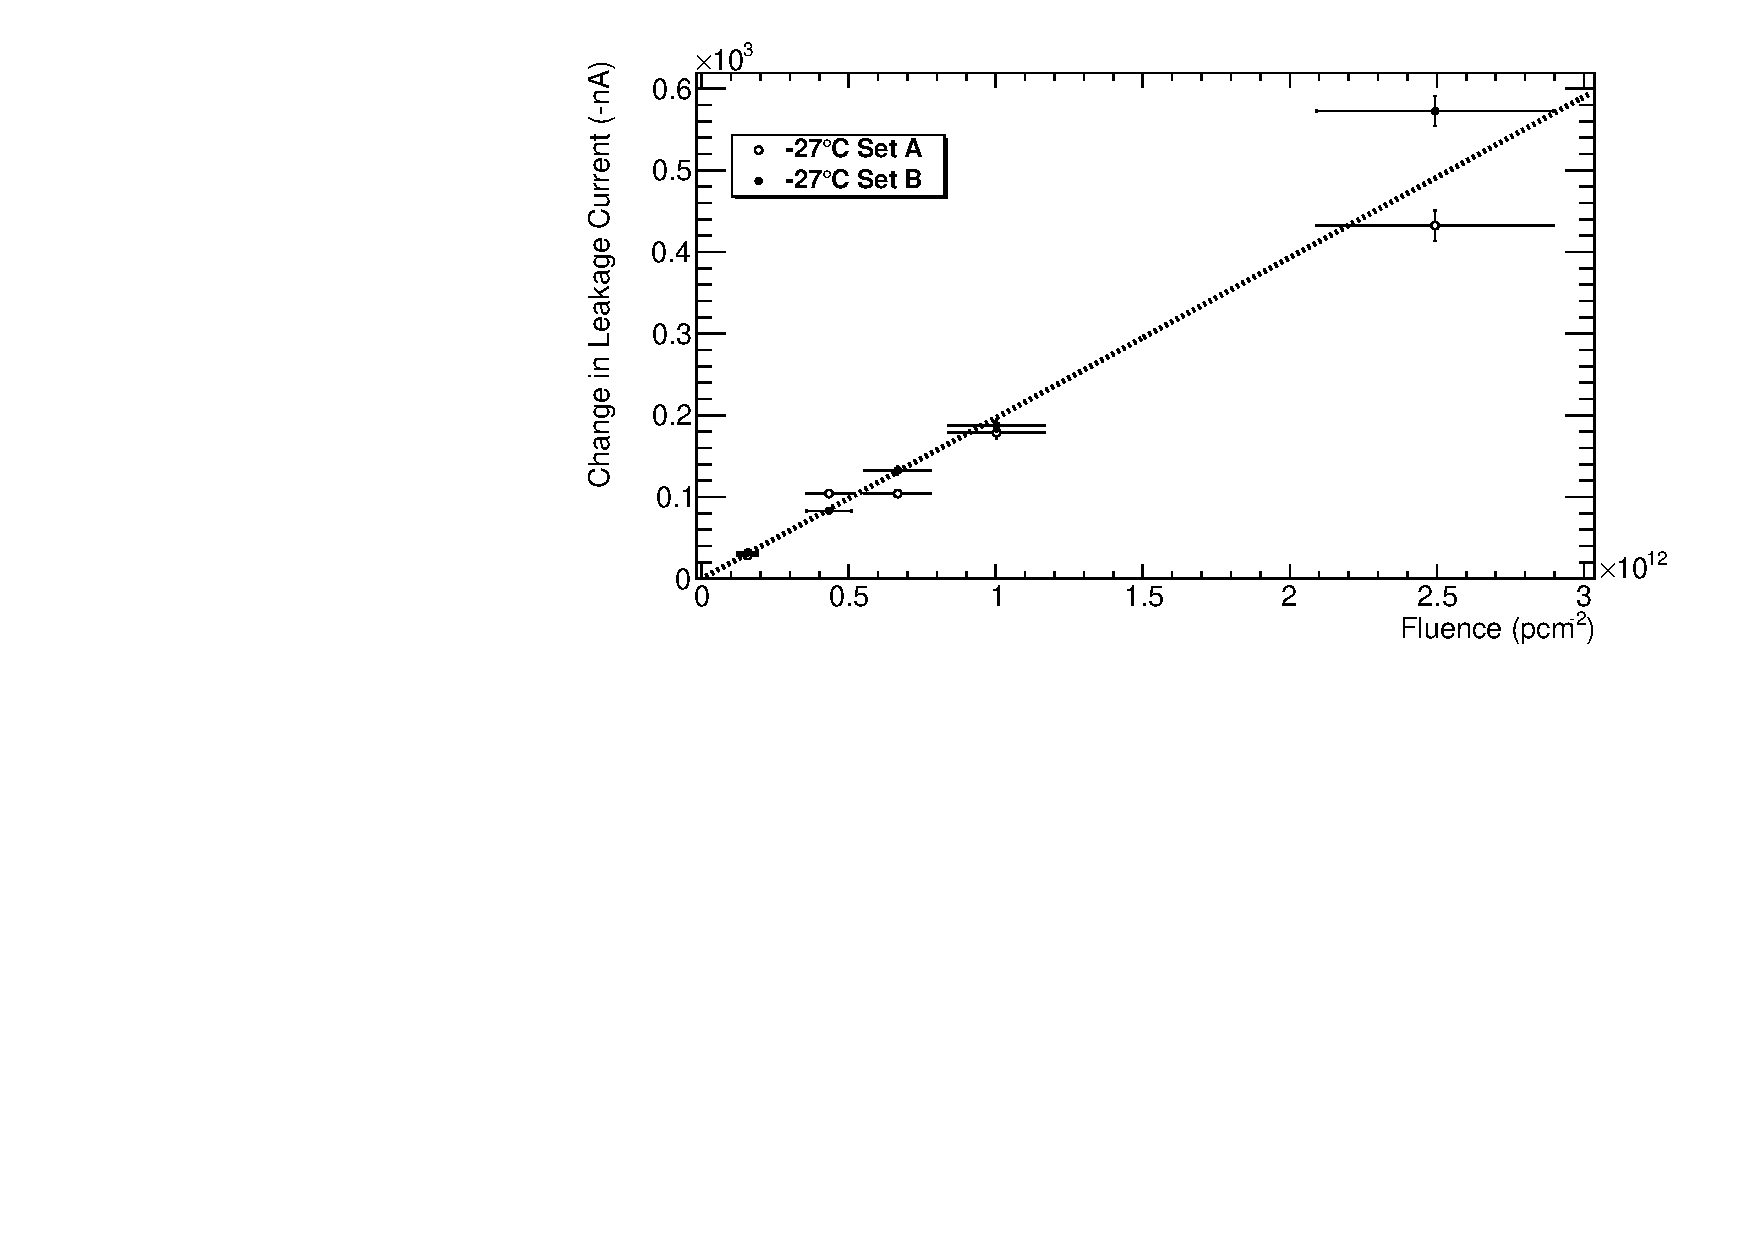
\includegraphics[width=0.9\linewidth]{Leakage_Fluence_Combined_Cold_0603.pdf}
            \caption{Change in leakage current vs proton fluence for $-27^{\circ}$C data.}
        \end{figure}
    \end{frame}
    
    \begin{frame}{Appendix: Determining the Hardness Factor}{Results for KIT}
        \begin{figure}
            \centering
            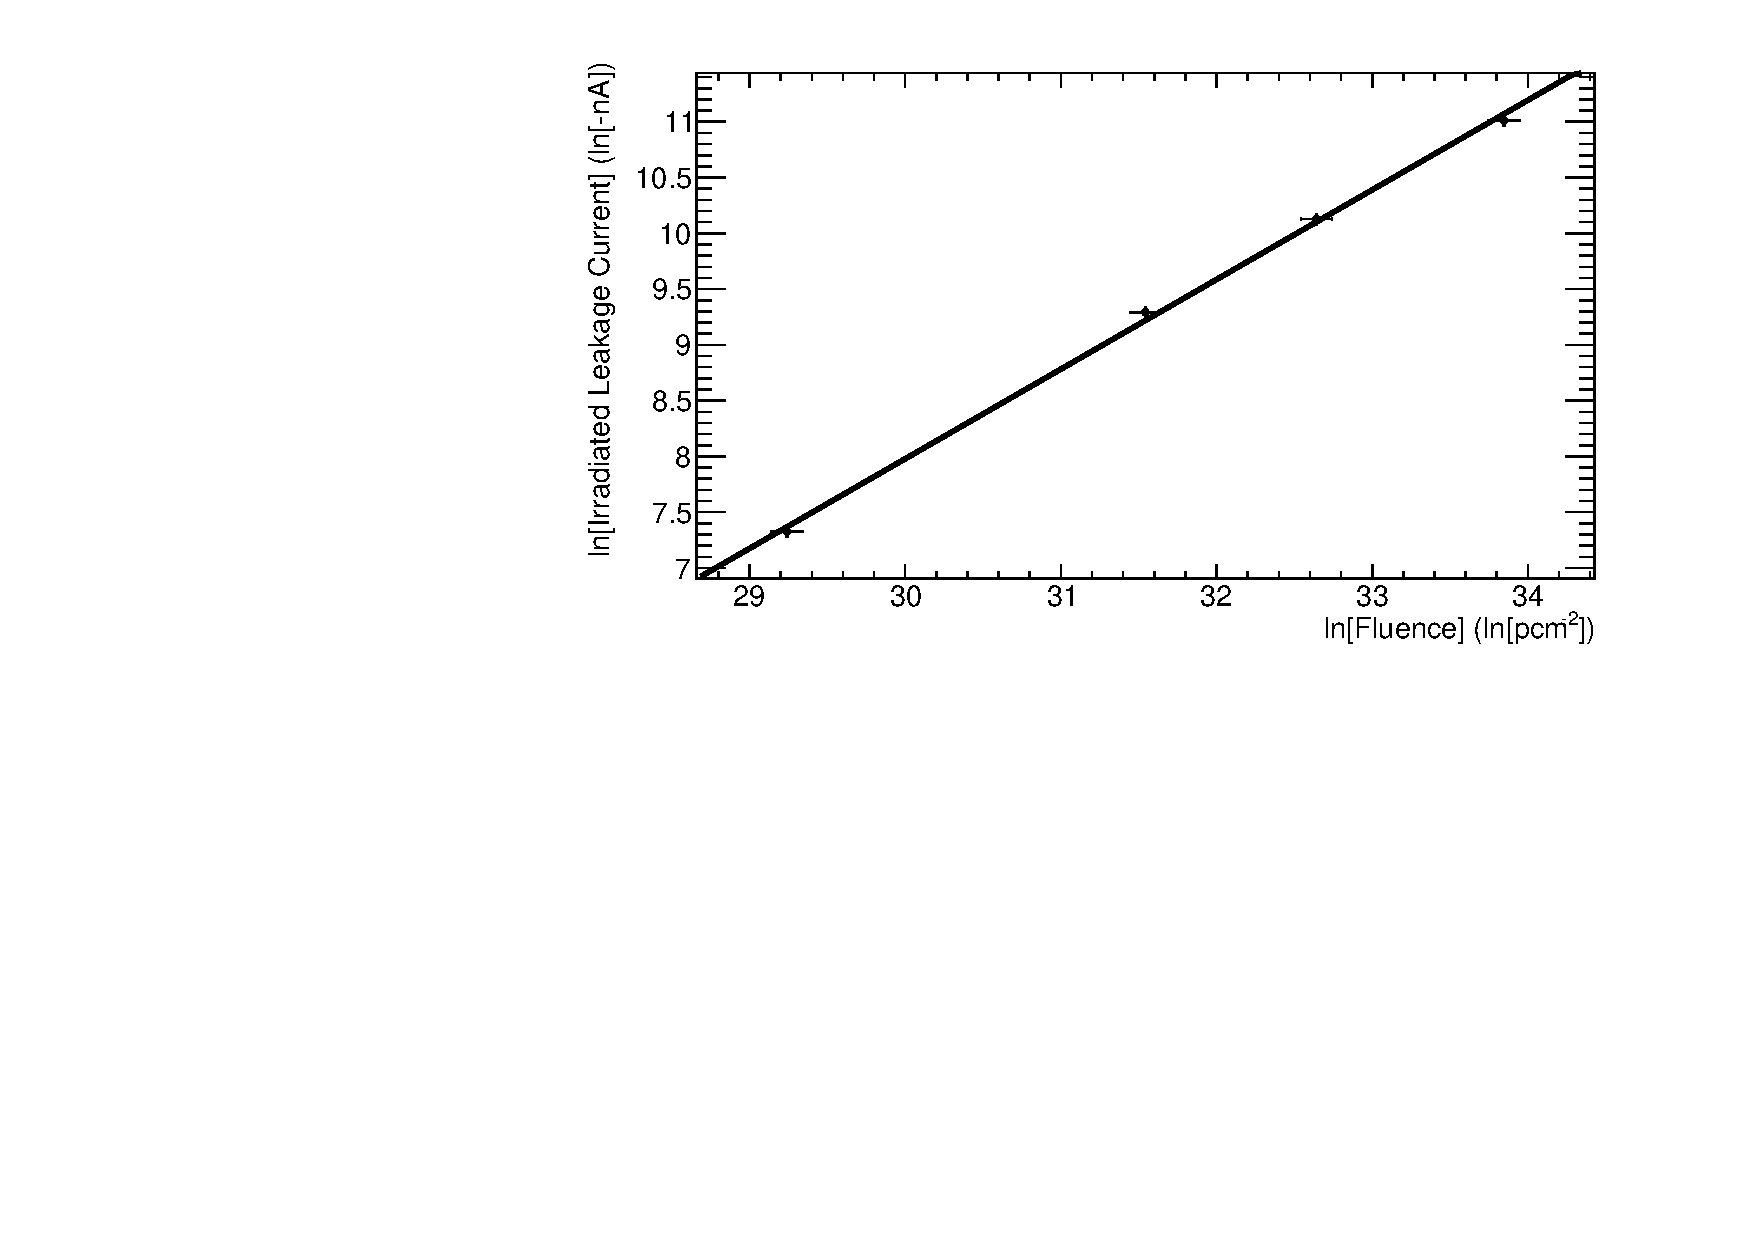
\includegraphics[width=0.9\linewidth]{KIT_deltaI_fluence_2302_log.pdf}
            \caption{Log of irradiated leakage current vs log of proton fluence for KIT photodiodes.}
        \end{figure}
    \end{frame}
    
% ADD IN NUMBERS
% IRRAD?
% Recommendations for the future.
% Appendix - Hardness factor with all points and KIT
\end{document}


